\chapter{Stratégie d'analyse des propriétés CP du boson de Higgs}
\label{chap6}

Ce chapitre présente les méthodes et les outils nécessaires à l'étude des propriétés CP du boson de Higgs dans des collisions proton-proton. Ce travail s'inscrit à la suite de l'analyse de la structure CP du couplage de Yukawa du lepton tau \cite{Htautau}, réalisée avec les 137 fb$^{-1}$ de données collectées par le détecteur CMS lors de la seconde phase d'exploitation du LHC entre 2016 et 2018. Parmi les méthodes expérimentales mises en oeuvre pour réaliser cette mesure, cette analyse intègre également le déploiement pour la première fois de la méthode du vecteur polarimétrique dans le canal de désintégration $\tau_h\tau_h\rightarrow a_1^{3pr}+a_1^{3pr}$. Les bonnes performances de cette méthode montrées dans le travail de thèse de Guillaume Bourgatte \cite{guigui} ont motivé à étudier les possibilités de son déploiement dans d'autres canaux. Le chapitre commence par une présentation des méthodes expérimentales de mesure de l'état CP et du vecteur polarimétrique, puis des algorithmes de reconstruction des leptons tau. Ce travail inclut également une étude des variables optimales de spin du lepton tau ainsi que des performances du vecteur polarimétrique dans les canaux de désintégration hadroniques et semi-leptoniques.

\section{Méthodes expérimentales de mesure de l'état CP}
\label{CPmethods}

D'après la section \ref{violCP} mettant en avant l'enjeu des corrélations des composantes transverses de spin dans les désintégrations du boson de Higgs, il est possible d'extraire une observable $\phi_{CP}$ définie comme l'angle entre les plans de désintégration des leptons taus tels que vus dans le référentiel du boson de Higgs au repos. De la même façon que pour l'étude de la polarisation du lepton tau, l'état d'hélicité dicte une cinématique particulière à ses produits de désintégration et l'étude des corrélations angulaires entre les plans de désintégration de ces derniers fournit une sensibilité directe à la nature CP de l'interaction. La section efficace différentielle selon $\phi_{CP}$ de la désintégration $H\rightarrow \tau\tau$ peut alors s'écrire en fonction de $\alpha^{H\tau\tau}$ de la façon suivante :

\begin{equation}
    \frac{d\Gamma}{d\phi_{CP}}\sim 1-b(E^+)b(E^-)\frac{\pi^2}{16}\cos(\phi_{CP}-2\alpha^{H\tau\tau}),
\label{crosssection}
\end{equation}

où $b(E^+)$ et $b(E^-)$ sont des fonctions dépendantes de l'énergie des leptons taus. La figure \ref{phiCP2} présente la distribution de $\phi_{CP}$ pour différentes hypothèses dans le mode de désintégration $\tau_h\tau_h\rightarrow\pi\pi$, l'angle est ainsi défini par les plans contenant chacun un lepton tau et le pion issu de sa désintégration. La mesure de $\phi_{CP}$ permet alors d'accéder à la valeur de l'angle de mélange puisque le décalage de phase entre la distribution obtenue et celle attendue dans le cadre du modèle standard lorsque $\alpha^{H\tau\tau}=0^{\circ}$ est égal à $2\alpha^{H\tau\tau}$. Il est également important de noter que les désintégrations issues du bruit de fond irréductible lié au boson $Z$ entraînent une distribution plate de $\phi_{CP}$ en raison de la nature vectorielle de ce dernier. La nature composite du proton combinée à la présence de neutrinos dans les désintégrations du lepton tau rend la reconstruction de son impulsion et du référentiel au repos du boson de Higgs difficile. Bien que cette technique d'analyse fut d'abord pensée pour fonctionner sur des collisionneurs de type électron-positron, il est possible de s'affranchir des difficultés liées a l'opération d'un collisionneur de hadrons tel que le LHC grâce à des techniques optimisées décrites dans les paragraphes suivants.\\

\begin{figure}
\centering
    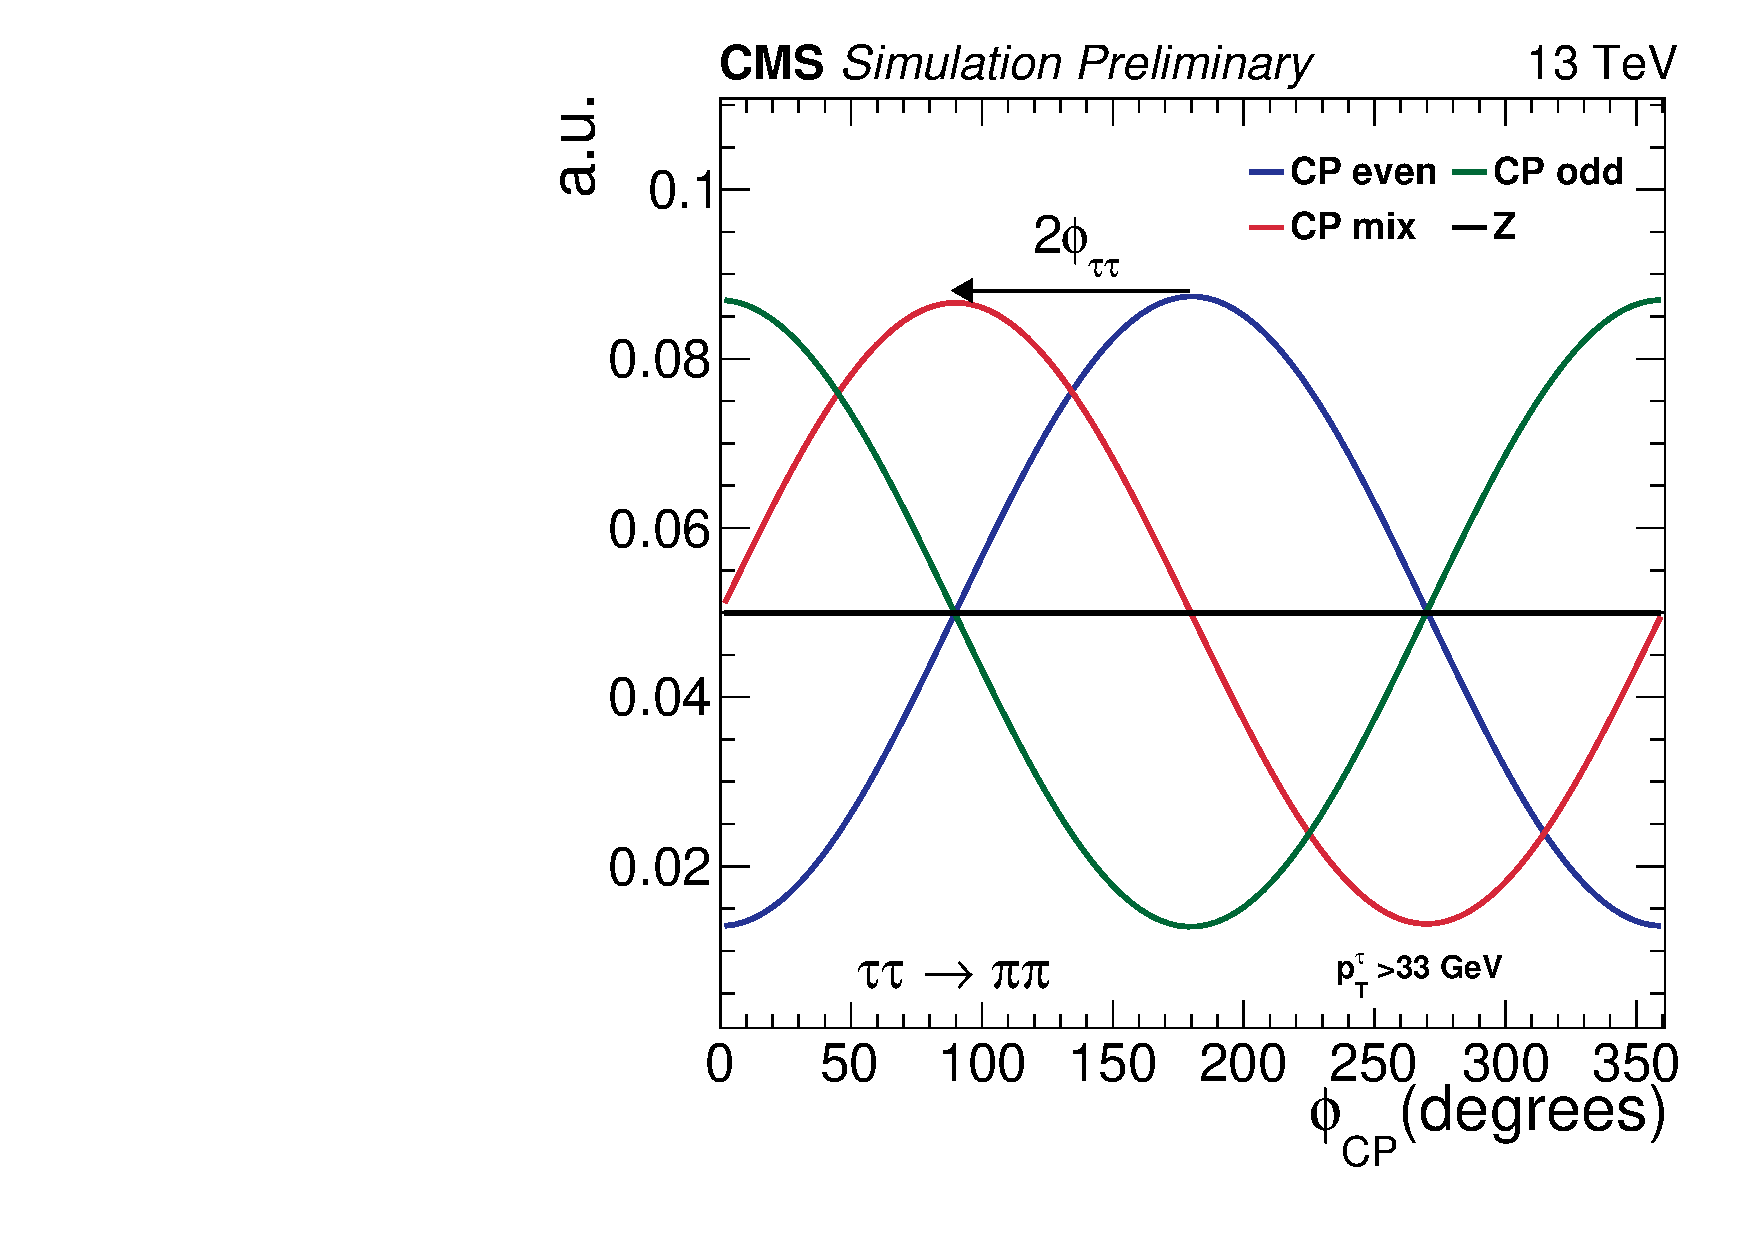
\includegraphics[scale=0.5]{Chapitre6/Images/Figure_001.pdf} 
    \caption{Distribution de l'angle acoplanaire $\phi_{CP}$ pour $\alpha^{H\tau\tau}=0^{\circ}$ (bleu), $\alpha^{H\tau\tau}=45^{\circ}$ (rouge) et $\alpha^{H\tau\tau}=90^{\circ}$ (vert) avec $\phi_{\tau\tau}\equiv\alpha^{H\tau\tau}$. La ligne plate noire représente la même distribution dans le cas d'une désintégration $Z/\gamma^*\rightarrow\tau\tau$ \cite{Htautau}.}
    \label{phiCP2}
\end{figure}

\subsection{Méthode du paramètre d'impact}
\label{IPmethod}

Cette première méthode est appliquée aux modes de désintégration du lepton tau à une particule chargée $\bigl(\tau^{\pm}\rightarrow\pi^{\pm}(\nu_{\tau}),\mu^{\pm}(\nu_{\tau}\nu_{\mu})\bigr)$ en s'appuyant sur la reconstruction du paramètre d'impact. Idéalement, ce dernier correspond au vecteur $\vb*{j}$ défini selon la distance minimale d'approche entre le vertex primaire et l'extrapolation de la trace reconstruite de la particule chargée depuis le vertex secondaire (Fig. \ref{IP}). Le vertex secondaire ne pouvant être cependant reconstruit que dans les états finaux à trois particules chargées, une procédure générale de reconstruction du paramètre d'impact est décrite dans la section \ref{IPreco} pour les pions et les muons. \\

\begin{figure}[!ht]
\centering
    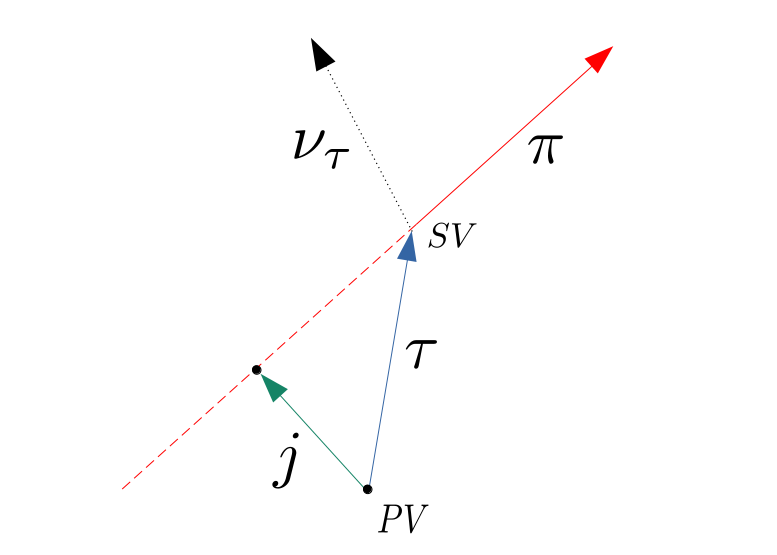
\includegraphics[scale=0.4]{Chapitre6/Images/IP.png} 
    \caption{Schéma du paramètre d'impact $\vb*{j}$ d'un pion issu du vertex secondaire (SV) entre sa trace extrapolée et le vertex primaire (PV).}
    \label{IP}
\end{figure}

La suite de la méthode consiste à mesurer l'angle entre les composantes transverses de chaque paramètre d'impact tel que vu dans le référentiel d'impulsion nulle (ZMF, \textit{Zero Momentum Frame}) constitué par la somme des impulsions quadrivectorielles des deux particules chargées. Chaque paramètre d'impact $\vb{j}^{\pm}$ est dans un premier temps exprimé sous une forme quadrivectorielle $\lambda^{\pm}=(\vb{j}^{\pm},0)$ puis boosté dans le ZMF et noté $\lambda^{\pm*}$. Chaque particule chargée est elle aussi boostée dans le ZMF puis notée $q^{\pm*}$. On défini ensuite les angles $\phi^*$ et $O^*$ à partir de la composante transverse $\lambda_{\perp}^{\pm*}$ de $\lambda^{\pm*}$ par rapport à $q^{\pm*}$ puis en utilisant le vecteur unitaire selon la direction de chaque composant :

\begin{equation}
    \left\{
    \begin{array}{ll}
        \phi^*=\arccos(\hat{\lambda}^{*+}_{\perp}\cdot \hat{\lambda}^{*-}_{\perp}), \\
        O^*=\hat{q}^{*-}\cdot(\hat{\lambda}^{*+}_{\perp}\times\hat{\lambda}^{*-}_{\perp}).
    \end{array}
    \right.
    \label{phistar}
\end{equation} 

Enfin, $\phi_{CP}$ est défini dans l'intervalle $[0,2\pi]$ à partir des angles précédents selon :

\begin{equation}
\phi_{CP}=
    \left\{
    \begin{array}{ll}
        \phi^* & \mbox{si} \; O^*\geq0, \\
        2\pi - \phi^* & \mbox{si} \; O^*<0.
    \end{array}
    \right.
    \label{phicp}
\end{equation} 

\subsection{Méthode du pion neutre}

La méthode du pion neutre est applicable aux modes de désintégration comportant au moins une particule chargée et une particule neutre dans l'état final. Elle s'applique notamment dans le mode de désintégration $\tau^{\pm}_h\rightarrow\pi^{\pm}\pi^0$ de la même façon que la méthode décrite dans la section \ref{IPmethod} en donnant au pion neutre le rôle de paramètre d'impact. Elle peut également s'utiliser dans les modes de désintégration $\tau^{\pm}_h\rightarrow a_1^{\pm}$ en utilisant le plan défini par les particules chargées issues de la désintégration de la résonance intermédiaire $\rho^0$ (Fig. \ref{rho0plane}) et en donnant au pion de charge opposée à la résonance $a_1$ le rôle de pion neutre dans le cas d'une désintégration à trois particules chargées, ou la somme des impulsions des deux pions neutres dans le cas d'une désintégration à une particule chargée. La méthode peut également être désignée par méthode des plans de désintégration (\textit{decay plane method}) lorsqu'elle est appliquée à la résonance $a_1^{3pr}$. \\

\begin{figure}[!ht]
\centering
    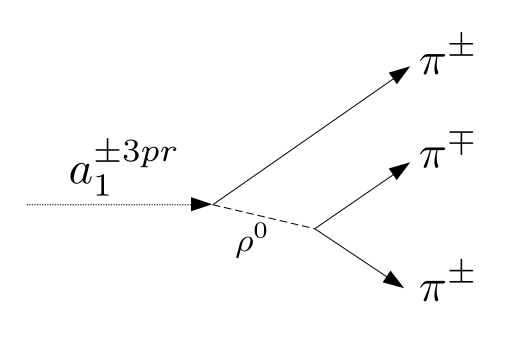
\includegraphics[scale=0.5]{Chapitre6/Images/rhoDP.png} 
    \caption{Chaîne de désintégration de la résonance $a_1^{3pr}$.}
    \label{rho0plane}
\end{figure}

La méthode du pion neutre se différencie toutefois de la méthode du paramètre d'impact par l'ajout de nouvelles variables permettant de caractériser la polarisation des leptons taus et d'éviter les interférences négatives entre états de polarisation différents :

\begin{equation}
    \left\{
    \begin{array}{ll}
        y^{\tau^-}=\frac{E_{\pi^-}-E_{\pi^0}}{E_{\pi^-}+E_{\pi^0}}, \\
        y^{\tau^+}=\frac{E_{\pi^+}-E_{\pi^0}}{E_{\pi^+}+E_{\pi^0}}, \\
        y^{\tau}=y^{\tau^-}y^{\tau^+}.
    \end{array}
    \right.
\end{equation} 

L'observable $\phi_{CP}$ est ensuite calculée selon \ref{phistar} et \ref{phicp}, puis la règle suivante est appliquée : \\

\begin{equation}
\phi_{CP}=
    \left\{
    \begin{array}{ll}
        \phi_{CP} & \mbox{si} \; y^{\tau}\geq0, \\
        2\pi - \phi_{CP} & \mbox{si} \; y^{\tau}<0.
    \end{array}
    \right.
\end{equation}

La méthode du paramètre d'impact et celle du pion neutre sont représentées schématiquement dans la figure \ref{CPmethods}, ainsi que la combinaison de ces deux méthodes applicable dans le cas où les deux leptons tau se désintègrent selon des canaux différents.


\begin{figure}
\centering
    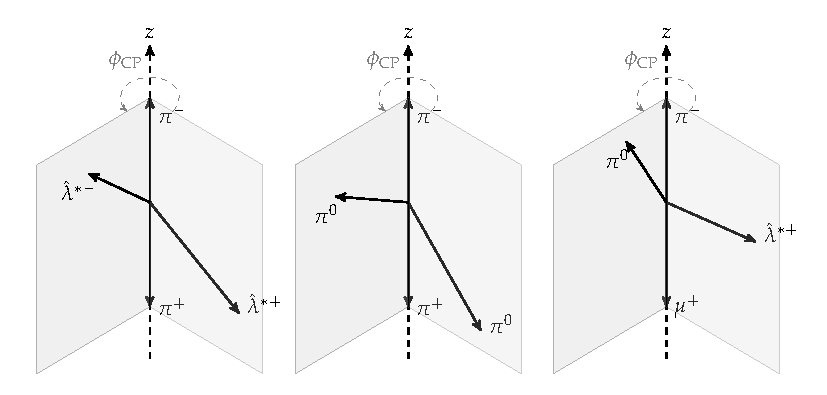
\includegraphics[scale=0.9]{Chapitre6/Images/Figure_002.pdf} 
    \caption{Définition des plans de désintégration et de l'angle $\phi_{CP}$ dans le référentiel des particules chargées pour la méthode du paramètre d'impact (gauche0, du pion neutre (centre) et de la combinaison des deux methodes (droite) \cite{Htautau}.}
    \label{CPmethods}
\end{figure}

\subsection{Méthode du vecteur polarimétrique}

Le quadrivecteur polarimétrique $h_{\mu}$ d'un lepton tau intervient dans l'expression de son taux de désintégration $d\Gamma$ conjointement à son quadrivecteur de spin $s_{\mu}$ de telle sorte que 

\begin{equation}
    d\Gamma\propto(1-h_{\mu}s^{\mu}).
    \label{dGamma}
\end{equation}

Dans le référentiel au repos du lepton tau où $s^0=0$, le produit scalaire $h_{\mu}s^{\mu}$ devient simplement égal à l'opposé du produit scalaire de chaque composante spatiale $-\vb{h}\cdot\vb{s}$. On remarque alors que $d\Gamma$ est maximisé lorsque le spin $\vb{s}$ du lepton tau et son vecteur polarimétrique $\vb{h}$ sont alignés. De cette façon, le vecteur polarimétrique peut être considéré comme la direction la plus probable du spin du tau dans son référentiel au repos et constitue une sonde solide dans l'analyse des corrélations de spin. Il peut être reconstruit expérimentalement grâce à l'impulsion des produits de désintégration du tau et aux modèles de désintégration des résonances impliquées, basés sur les variables angulaires définies dans la section \ref{tau properties}. L'expression générale du vecteur polarimétrique pour les différents modes de désintégration est explicitée dans la référence \cite{cherepanov2018methods}. Les plans sont ensuite définis par le vecteur unitaire selon la direction du vecteur polarimétrique $\hat{\vb{h}}_{1,2}$ et le vecteur unitaire selon la direction du tau $\hat{\vb{n}}_{1,2}$ dans le référentiel au repos du boson de Higgs. L'angle entre ces plans est alors calculé selon les relations suivantes :

\begin{equation}
\phi^*=\arccos(\hat{\vb{k}}_1\cdot\hat{\vb{k}}_2), 
\end{equation}

avec $\hat{\vb{k}}_{1,2}=\frac{\hat{\vb{h}}_{1,2}\times\hat{\vb{n}}_{1,2}}{|\hat{\vb{h}}_{1,2}\times\hat{\vb{n}}_{1,2}|}.$ \\

L'angle $\phi_{CP}$ est finalement donné par :

\begin{equation}
\phi_{CP}=
    \left\{
    \begin{array}{ll}
        \phi_{CP} & \mbox{si} \; (\hat{\vb{h}}_{1}\times\hat{\vb{h}}_{2})\cdot\hat{\vb{n}}_{1}\leq0, \\
        2\pi - \phi_{CP} & \mbox{si} \; (\hat{\vb{h}}_{1}\times\hat{\vb{h}}_{2})\cdot\hat{\vb{n}}_{1}>0.
    \end{array}
    \right.
\end{equation}

Cette méthode est en théorie applicable à tout mode de désintégration hadronique du lepton tau mais implique la reconstruction de l'impulsion de ce dernier ainsi que la reconstruction du référentiel au repos du boson de Higgs. Cette condition rend son application difficile dans la plupart des canaux malgré sa haute sensibilité avérée. Le prochain paragraphe sera dédié à la présentation des performances du vecteur polarimétrique en comparaison des méthodes du paramètre d'impact et du pion neutre ainsi que les limites actuelles d'application.

\section{Simulation de l'état CP}
\label{CPsim}

Afin de simuler les différents états CP du boson de Higgs, des échantillons Monte Carlo de signal dans lesquels les désintégrations $H\rightarrow\tau\tau$ sont simulées sans effets de corrélation du spin sont utilisés. À la place, le module \textsc{Tauspinner} \cite{Czyczula2012,Przedzinski2014} est employé pour simuler ces effets \textit{a posteriori} par repondération des évènements et permettant ainsi de produire un scénario pour toute valeur de l'angle de mélange $\alpha^{H\tau\tau}$ à partir d'un échantillon commun. D'après \ref{crosssection}, la section efficace différentielle de la désintégration $H\rightarrow\tau\tau$ possède une forme sinusoïdale de la forme 

\begin{equation}
    \frac{d\sigma}{d\phi_{CP}}\propto const-\cos\bigl(\phi_{CP}-2\alpha^{H\tau\tau}\bigr),
\end{equation}

pouvant se réécrire à un facteur de normalisation près sous la forme

\begin{align*}
    \frac{d\sigma}{d\phi_{CP}} & \sim-\cos\bigl(2\alpha^{H\tau\tau}\bigr)\cos\bigl(\phi_{CP}\bigr)-\sin\bigl(2\alpha^{H\tau\tau}\bigr)\sin\bigl(\phi_{CP}\bigr) \\
    & = -\bigl(\cos^2\bigl(\alpha^{H\tau\tau}\bigr)-\sin^2\bigl(\alpha^{H\tau\tau}\bigr)\bigr)\cos\bigl(\phi_{CP}\bigr)-\sin\bigl(\alpha^{H\tau\tau}\bigr)\cos\bigl(\alpha^{H\tau\tau}\bigr)\sin\bigl(\phi_{CP}\bigr).
\end{align*}

Cette expression représente une somme pondérée de $\cos(\phi_{CP})$ et $\sin(\phi_{CP})$ et permet d'exprimer la section efficace différentielle pour toute valeur de $\alpha^{H\tau\tau}$ à partir de seulement trois modèles dans lesquels la valeur de $\alpha^{H\tau\tau}$ est fixée. En choisissant les trois scénarios représentés dans la figure \ref{phicp}, à savoir le cas CP pair ($\alpha^{H\tau\tau}=0^\circ$), le cas CP impair ($\alpha^{H\tau\tau}=90^\circ$) et le cas pour lequel la violation CP est maximale ($\alpha^{H\tau\tau}=45^\circ$), on obtient :

\begin{align}
    \frac{d\sigma^{CP-even}}{d\phi_{CP}} & \sim -\cos\bigl(\phi_{CP}\bigr), \\[1em]
    \frac{d\sigma^{CP-odd}}{d\phi_{CP}} & \sim \cos\bigl(\phi_{CP}\bigr), \\[1em]
    \frac{d\sigma^{CP-mix}}{d\phi_{CP}} & \sim \sin\bigl(\phi_{CP}\bigr).   
\end{align}

On obtient alors une expression paramétrique générale de la section efficace différentielle à partir d'un échantillon sans corrélations de spin et de trois poids calculés par le module \textsc{Tauspinner} :

\begin{align}
    \frac{d\sigma}{d\phi_{CP}} & \sim \bigl(\cos^2\bigl(\alpha^{H\tau\tau}\bigr)-\sin\bigl(\alpha^{H\tau\tau}\bigr)\cos\bigl(\alpha^{H\tau\tau}\bigr)\bigr)\frac{d\sigma^{CP-even}}{d\phi_{CP}} \nonumber \\[1em] 
     & + \bigl(\sin^2\bigl(\alpha^{H\tau\tau}\bigr)-\sin\bigl(\alpha^{H\tau\tau}\bigr)\cos\bigl(\alpha^{H\tau\tau}\bigr)\bigr)\frac{d\sigma^{CP-odd}}{d\phi_{CP}} \nonumber \\[1em] 
     & + 2\sin\bigl(\alpha^{H\tau\tau}\bigr)\cos\bigl(\alpha^{H\tau\tau}\bigr)\frac{d\sigma^{CP-mix}}{d\phi_{CP}}.
     \label{CPdiff}
\end{align}

\section{Reconstruction cinématique des évènements $H/Z\rightarrow\tau\tau$}
\label{taualgo}

Les méthodes de reconstruction et d'identification du lepton tau décrites précédemment ne concernent que la partie visible de sa désintégration. Afin de reconstruire des grandeurs telles que la masse invariante du boson de Higgs dans les désintégrations $H\rightarrow\tau\tau$, il est nécessaire d'effectuer une reconstruction complète de l'impulsion de chaque lepton tau tenant compte des neutrinos.

\subsection{Algorithmes SVFit et FastMTT}

L'algorithme SVFit \cite{SVFit} a été développé au sein de la collaboration CMS dans le but de mesurer avec précision la masse du boson de Higgs dans des évènements $H\rightarrow\tau\tau$ tout en offrant la meilleure séparation possible avec le bruit de fond dominant $Z\rightarrow\tau\tau$. La désintégration hadronique (leptonique) du lepton tau est paramétrisée par deux (trois) variables définies dans son référentiel au repos : 

\begin{itemize}
    \medskip
    \item[$\bullet$] $\theta_{\text{inv}}$, défini par l'angle polaire entre l'impulsion invisible et l'impulsion visible du tau,
    \medskip
    \item[$\bullet$] $\phi_{\text{inv}}$, défini par l'angle azimuthal entre la projection de l'impulsion invisible dans le plan transverse à l'impulsion visible et l'axe $x$,
    \medskip
    \item[$\bullet$] $m_{\nu\nu}$, définie par la masse invariante de la paire de neutrinos dans le cas d'une désintégration leptonique.
    \medskip
\end{itemize}

Au total, quatre variables sont à déterminer le canal $\tau_h\tau_h$, cinq pour le canal $\ell\tau_h$ et six pour le canal $\ell\ell$. Le système est quant à lui contraint par seulement 2 observables obtenues par la mesure des composantes de l'énergie transverse manquante $E_x^{\text{miss}}$ et $E_y^{\text{miss}}$. \\

Afin de mesurer la masse invariante $M_{\tau\tau}$, une approche par maximisation de la vraisemblance est appliquée évènement par évènement. Pour une série d'hypothèses de masse $M_{\tau\tau}$, l'algorithme vise à maximiser la fonction de vraisemblance suivante :

\begin{equation}
    \frac{dL(M_{\tau\tau})}{dM_{\tau\tau}}=\int \frac{df(\vb{x}_u|\vb{x}_m)}{d\vb{x}_u}\delta\bigl(M_{\tau\tau}-M_{\tau\tau}(\vb{x}_u,\vb{x}_m)\bigr)d\vb{x_u},
\end{equation}

où $\vb{x}_u$ représente les variables inconnues $\theta_{\text{inv}}$, $\phi_{\text{inv}}$, $m_{\nu\nu}$ et $\vb{x}_m$ les observables mesurées $E_x^{\text{miss}}$, $E_y^{\text{miss}}$ et $m_{\text{vis}}$ la masse visible du lepton tau. L'intégrale représente une moyenne effectuée sur tous les paramètres $\vb{x}_u$ pondérés par leur consistance avec les paramètres observés $\vb{x}_m$. L'algorithme SVFit offre une bonne résolution sur la masse invariante $M_{\tau\tau}$ (Fig. \ref{SVFitres}) mais souffre d'un temps de calcul long. Dans cet objectif, une version simplifiée nommée FastMTT a également été développée notamment dans laquelle le lepton tau et les neutrinos sont toujours considérés comme collinéaires.

\begin{figure}
\centering
    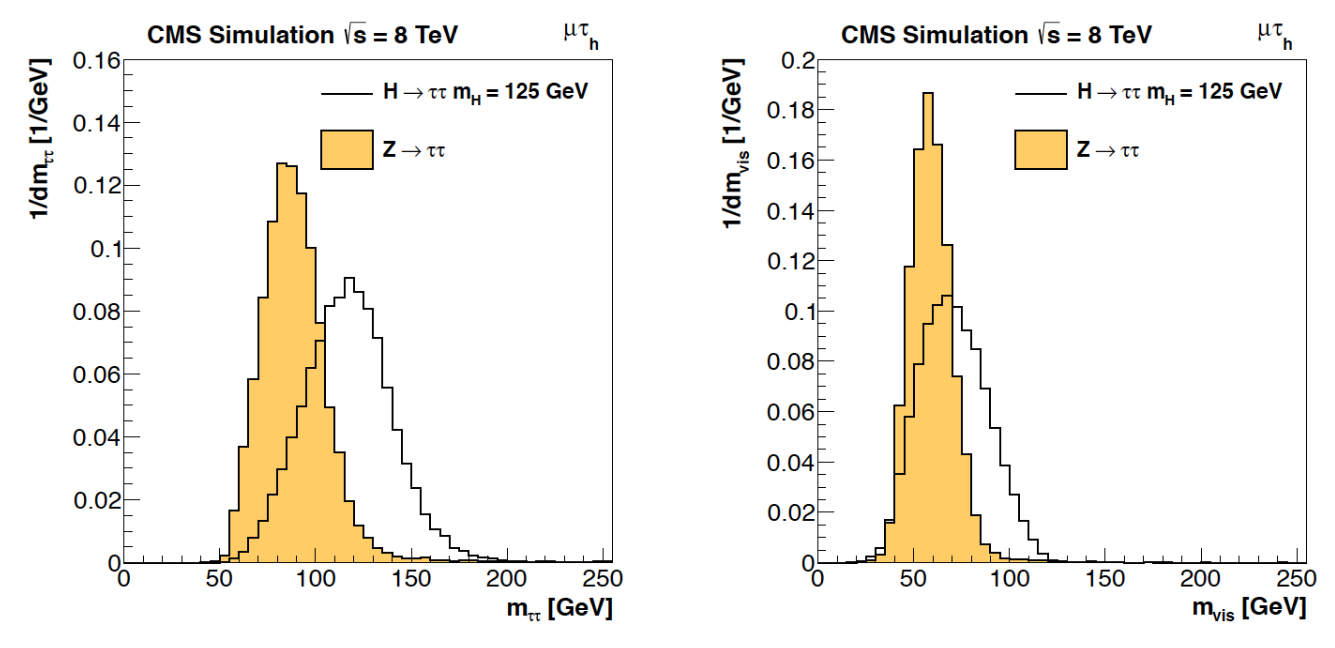
\includegraphics[scale=0.3]{Chapitre6/Images/SVFitres.png} 
    \caption{Distribution de $M_{\tau\tau}$ (gauche) reconstruite par SVFit et de la masse visible des leptons tau (droite), pour des évènements de signal $H\rightarrow\tau\tau$ et le bruit de fond $Z/\gamma^*\rightarrow\tau\tau$ dans le canal $\tau_h\mu$. \cite{SVFit}}
    \label{SVFitres}
\end{figure}

\subsection{Global Event Fit (GEF)}
\label{GEF}

L'algorithme GEF \cite{GEF} est basé sur une régression capable de reconstruire l'intégralité d'un évènement $H/Z\rightarrow\tau\tau$ dont l'état final contient au moins une résonance $a_1^{3pr}$. La procédure de reconstruction se déroule en trois étapes :

\begin{enumerate}
    \item Reconstruction du vertex primaire et du vertex secondaire du lepton $\tau\rightarrow\nu a_1^{3pr}$ ($\tau_1$).
    \item Calcul de l'impulsion de $\tau_1$.
    \item Régression cinématique de l'impulsion de la paire $\tau\tau$ avec plusieurs contraintes sur le système di-tau ($\tau_1+\tau_2$). 
\end{enumerate}

La procédure de reconstruction du vertex primaire (PV) est similaire à celle décrite dans la section \ref{PVreco}. La reconstruction du vertex secondaire (SV) repose sur l'hypothèse que le temps de vol de la résonance $a_1$ est nul. Les trois traces chargées issues de sa désintégration sont ensuite ajustées ensemble afin de définir un point d'origine commun. La direction du lepton $\tau_1$ peut ensuite être définie à partir de la position des deux vertex suivant :

\begin{equation}
    \vec{n}_{\tau}=\frac{\overrightarrow{SV}-\overrightarrow{PV}}{|\overrightarrow{SV}-\overrightarrow{PV}|}.
\end{equation}

Le calcul de l'impulsion du tau repose ensuite sur des principes de conservation de l'impulsion et l'énergie. En considérant un neutrino de masse nulle, il est possible d'écrire dans le référentiel du laboratoire :

\begin{equation}
    (P_{\tau}-P_{a_1})^2=0,
\end{equation}

où $P_{\tau/a_1}$ représente le quadrivecteur associé au lepton tau et à la résonance $a_1$ respectivement. L'impulsion du lepton tau peut alors s'écrire :

\begin{equation}
    |\vec{p_{\tau}}|=\frac{(m_{a_1}^2+m_{\tau}^2)|\vec{p_{a_1}}|\cos\theta_{GJ}\pm\sqrt{(m_{a_1}^2+\vec{p_{a_1}}^2)\bigl((m_{a_1}^2-m_{\tau}^2)^2-4m_{\tau}^2\vec{p_{a_1}}^2\sin^2\theta_{GJ}\bigr)}}{2(m_{a_1}^2+\vec{p_{a_1}}^2\sin^2\theta_{GJ})}
    \label{taup}
\end{equation}

où $\theta_{GJ}$, appelé angle de Gottfried-Jackson, représente l'angle entre la direction du lepton tau et la direction de la résonance $a_1$ dans le référentiel du laboratoire (Fig. \ref{thetaGF}). Pour un angle $\theta_{GJ}$ et une impulsion de la résonance $a_1$ donnés, il existe deux solutions pour l'impulsion du lepton tau. Il existe toutefois une valeur maximale $\theta_{GJ}^{\text{max}}$ de l'angle pour laquelle une seule solution existe lorsque le terme sous la racine de l'équation \ref{taup} est nul et donnée par :

\begin{equation}
    \theta_{GJ}^{\text{max}}=\arcsin\frac{m_{\tau}^2-m_{a_1}^2}{2m_{\tau}|\vec{p_{a_1}}|}.
\end{equation}

\begin{figure}
    \centering
    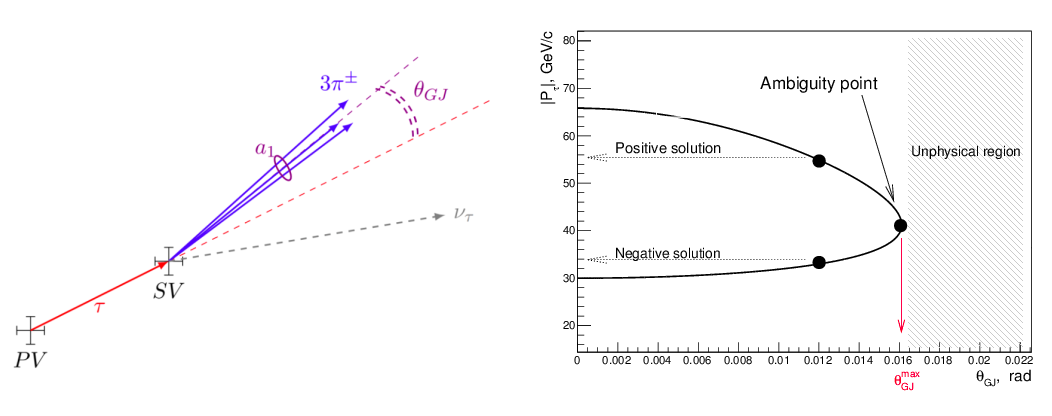
\includegraphics[scale=0.35]{Chapitre6/Images/thetaGF.png}
    \caption{Définition de l'angle $\theta_{GJ}$ (gauche) et sa dépendance à l'impulsion reconstruite (droite) \cite{GEF}.}
    \label{thetaGF}
\end{figure}

Les valeurs de $\theta_{GJ}$ étant généralement petites, une légère erreur de mesure sur la position des vertex peut conduire un évènement à se trouver dans une région non physique dans laquelle $\theta_{GJ}>\theta_{GJ}^{\text{max}}$ (Fig. \ref{thetaGF}). Le rejet de ces évènements causerait une perte de statistique importante, ainsi la direction du lepton tau est modifiée de sorte à rapporter $\theta_{GJ}$ à sa valeur maximale et une seule solution de $|\vec{p_{\tau}}|$ existe. Dans le cas où deux solutions existent $(\theta_{GJ}<\theta_{GJ}^{\text{max}})$, l'ambiguïté est levée lors de la régression itérative permettant de calculer l'impulsion du second lepton tau $\tau_2$. Cette seconde impulsion est calculée par minimisation d'une fonction de Lagrange dont l'expression est donnée par :

\begin{align}
\begin{split}
    \mathcal{L}(\vv{a},\vv{b},\vv{\lambda})&=\bigl(\vv{y}-\vv{a}\bigr)^{T}\vb{V}^{-1}_{y}\bigl(\vv{y}-\vv{a}\bigr) \\
    & +\vv{f}^{T}\bigl(\vv{a},\vv{b}\bigr)\vb{V}^{-1}_{f}\vv{f}\bigl(\vv{a},\vv{b}\bigr)\\
    & +2\vv{\lambda}^{T}\vv{H}\bigl(\vv{a},\vv{b}\bigr),
\end{split}
\end{align}

où $\vv{y}$ contient les paramètre de $\tau_1$ reconstruit dans la désintégration $\tau\to\nu a_1^{3pr}$, et $\vb{V_y}$ est la matrice de covariance associée. Les vecteurs $\vv{a}$ et $\vv{b}$ contiennent les paramètres après ajustement de $\tau_1$ et $\tau_2$, devant satisfaire les contraintes $\vv{H}(\vv{a},\vv{b})$ et $\vv{f}(\vv{a},\vv{b})$. Enfin $\vv{\lambda}$ représente les multiplicateurs de Lagrange. Dans ce formalisme, les paramètres de $\tau_1$ et $\tau_2$ sont déterminés lorsque la fonction $\mathcal{L}(\vv{a},\vv{b},\vv{\lambda})$ est minimale. Les contraintes sur le système sont divisées en deux catégories. La première regroupe les \textit{hard constraints} $\vv{H}$ sur la masse du système di-tau et sur l'impulsion transverse de $\tau_2$ :

\begin{equation} 
    \vv{H}=
    \begin{cases} 
    M_{\tau\tau} - M_{Z/H} & = 0 \\ 
    p_{z} - |\vv{p}_{2}|\cos\theta_2 & = 0, 
    \end{cases} 
\end{equation}

où $M_{\tau\tau}$ est la masse du système di-tau, $M_{Z/H}$ est la masse du boson $Z$ ou $H$, $p_z$ et $\vv{p}_2$ l'impulsion transverse et totale de $\tau_2$ et $\theta_2$ son angle polaire. La seconde regroupe les \textit{soft constraints} $\vv{f}$, tenant compte d'un éventuel boost transverse du boson $Z$ ou $H$ :

\begin{equation} 
    \vv{f}=
    \begin{cases} 
    p_x^{\tau_1}+p_x^{\tau_2}-p_x^{a_1}-p_x^{\text{vis}_2}-MET_x & = 0 \\ 
    p_y^{\tau_1}+p_y^{\tau_2}-p_y^{a_1}-p_y^{\text{vis}_2}-MET_y & = 0.
    \end{cases} 
\end{equation}

où chaque terme désigne respectivement l'impulsion selon la composante $x$ ou $y$ de $\tau_1$, de $\tau_2$, de la résonance $a_1$, de la partie visible de $\tau_2$ et enfin de la MET. \\

\begin{figure}[!ht]
  \begin{subfigure}[b]{0.5\linewidth}
    \centering
    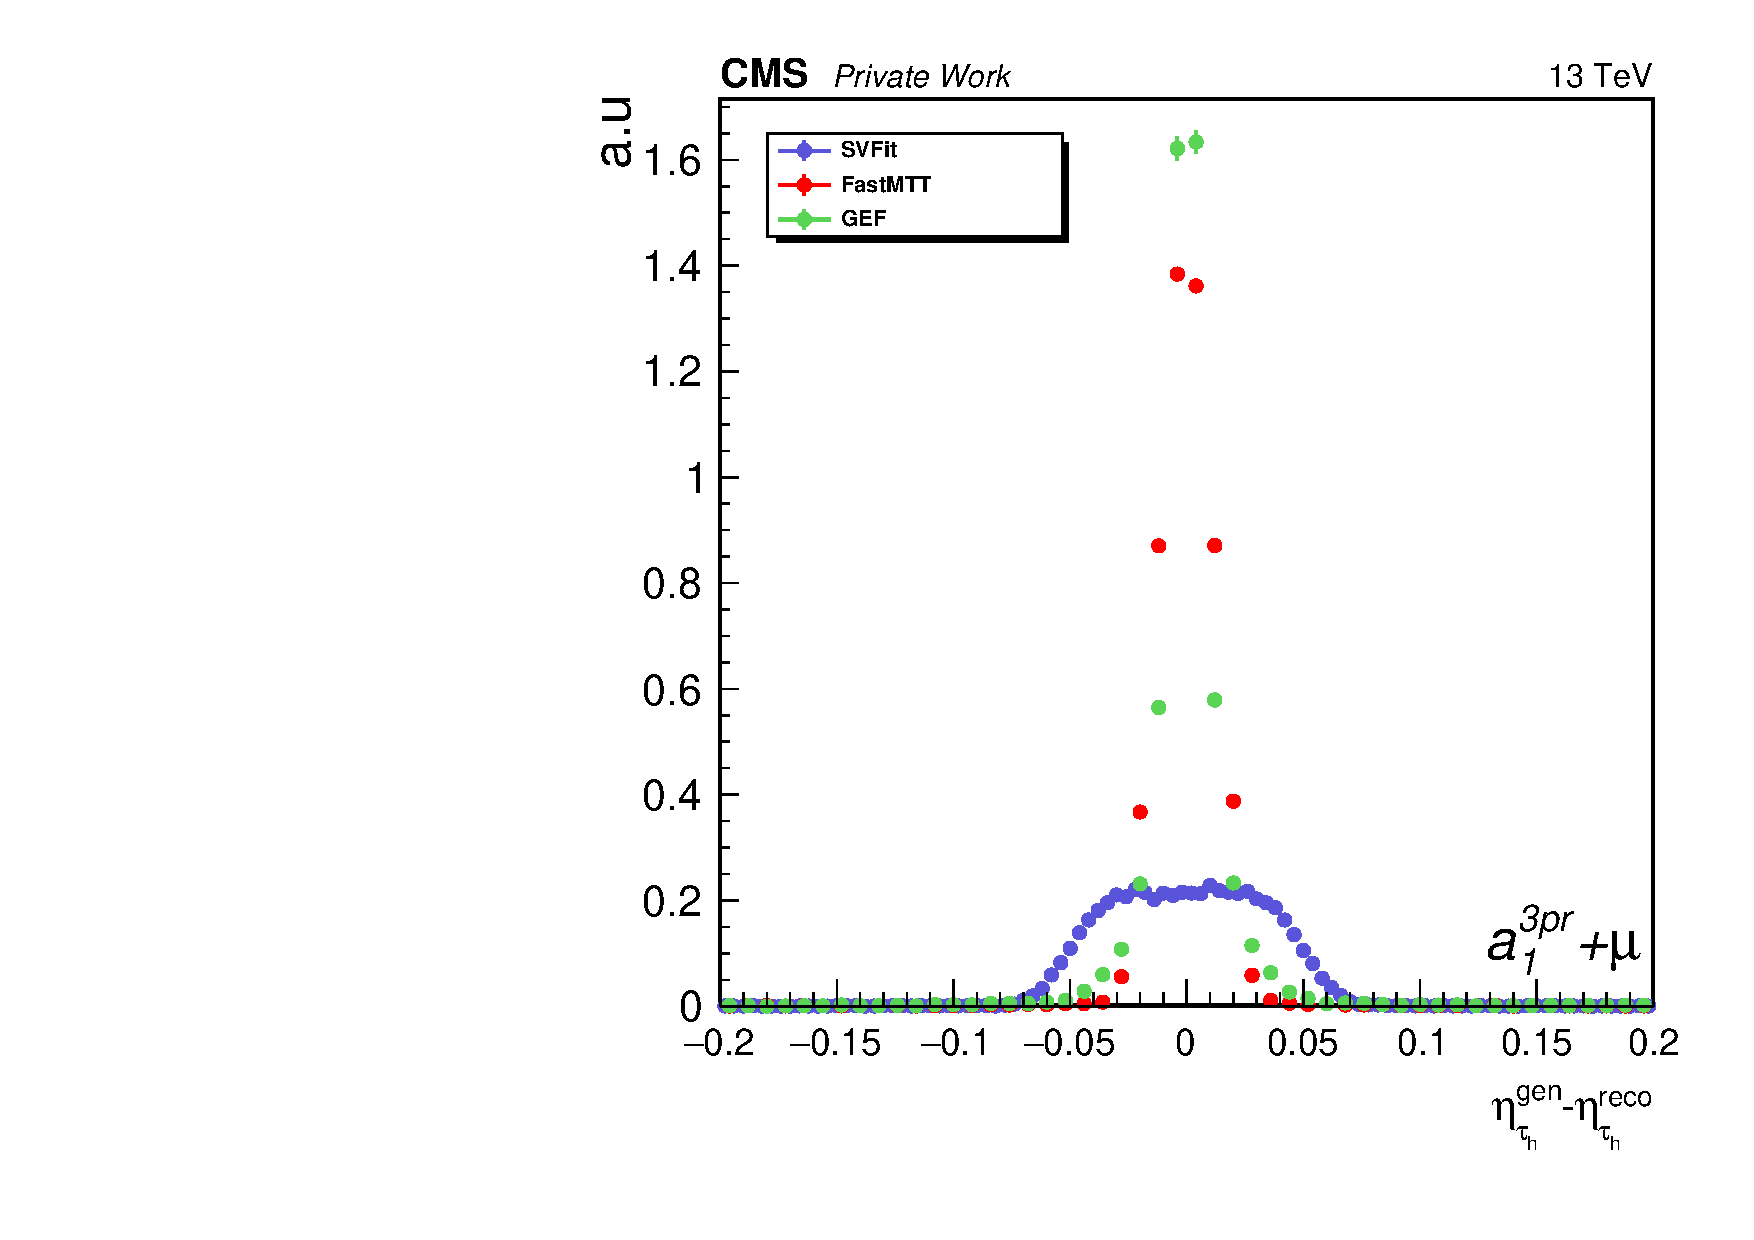
\includegraphics[width=\linewidth]{Chapitre6/Images/Eta.pdf} 
    \caption{} 
  \end{subfigure}%% 
  \begin{subfigure}[b]{0.5\linewidth}
    \centering
    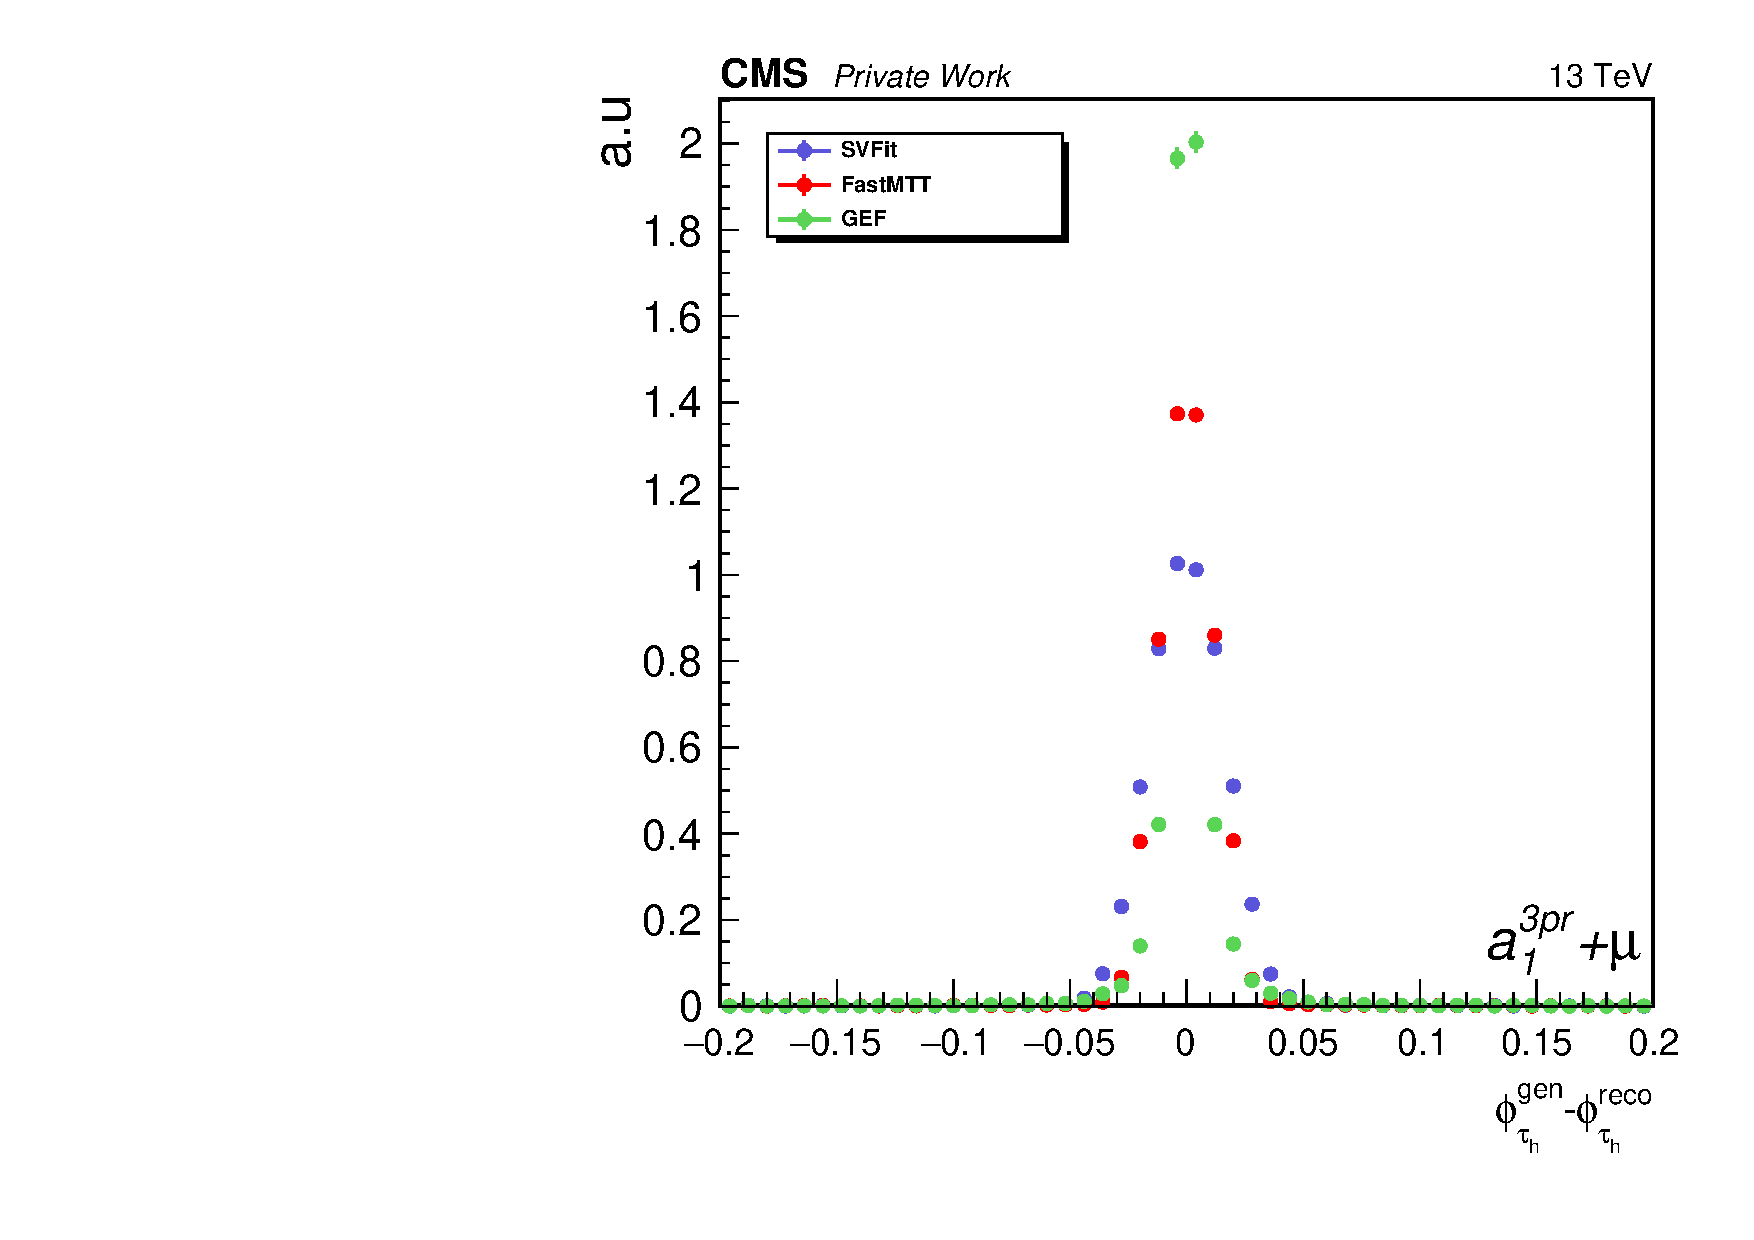
\includegraphics[width=\linewidth]{Chapitre6/Images/Phi.pdf} 
    \caption{} 
  \end{subfigure} 

  \begin{subfigure}[b]{0.5\linewidth}
    \centering
    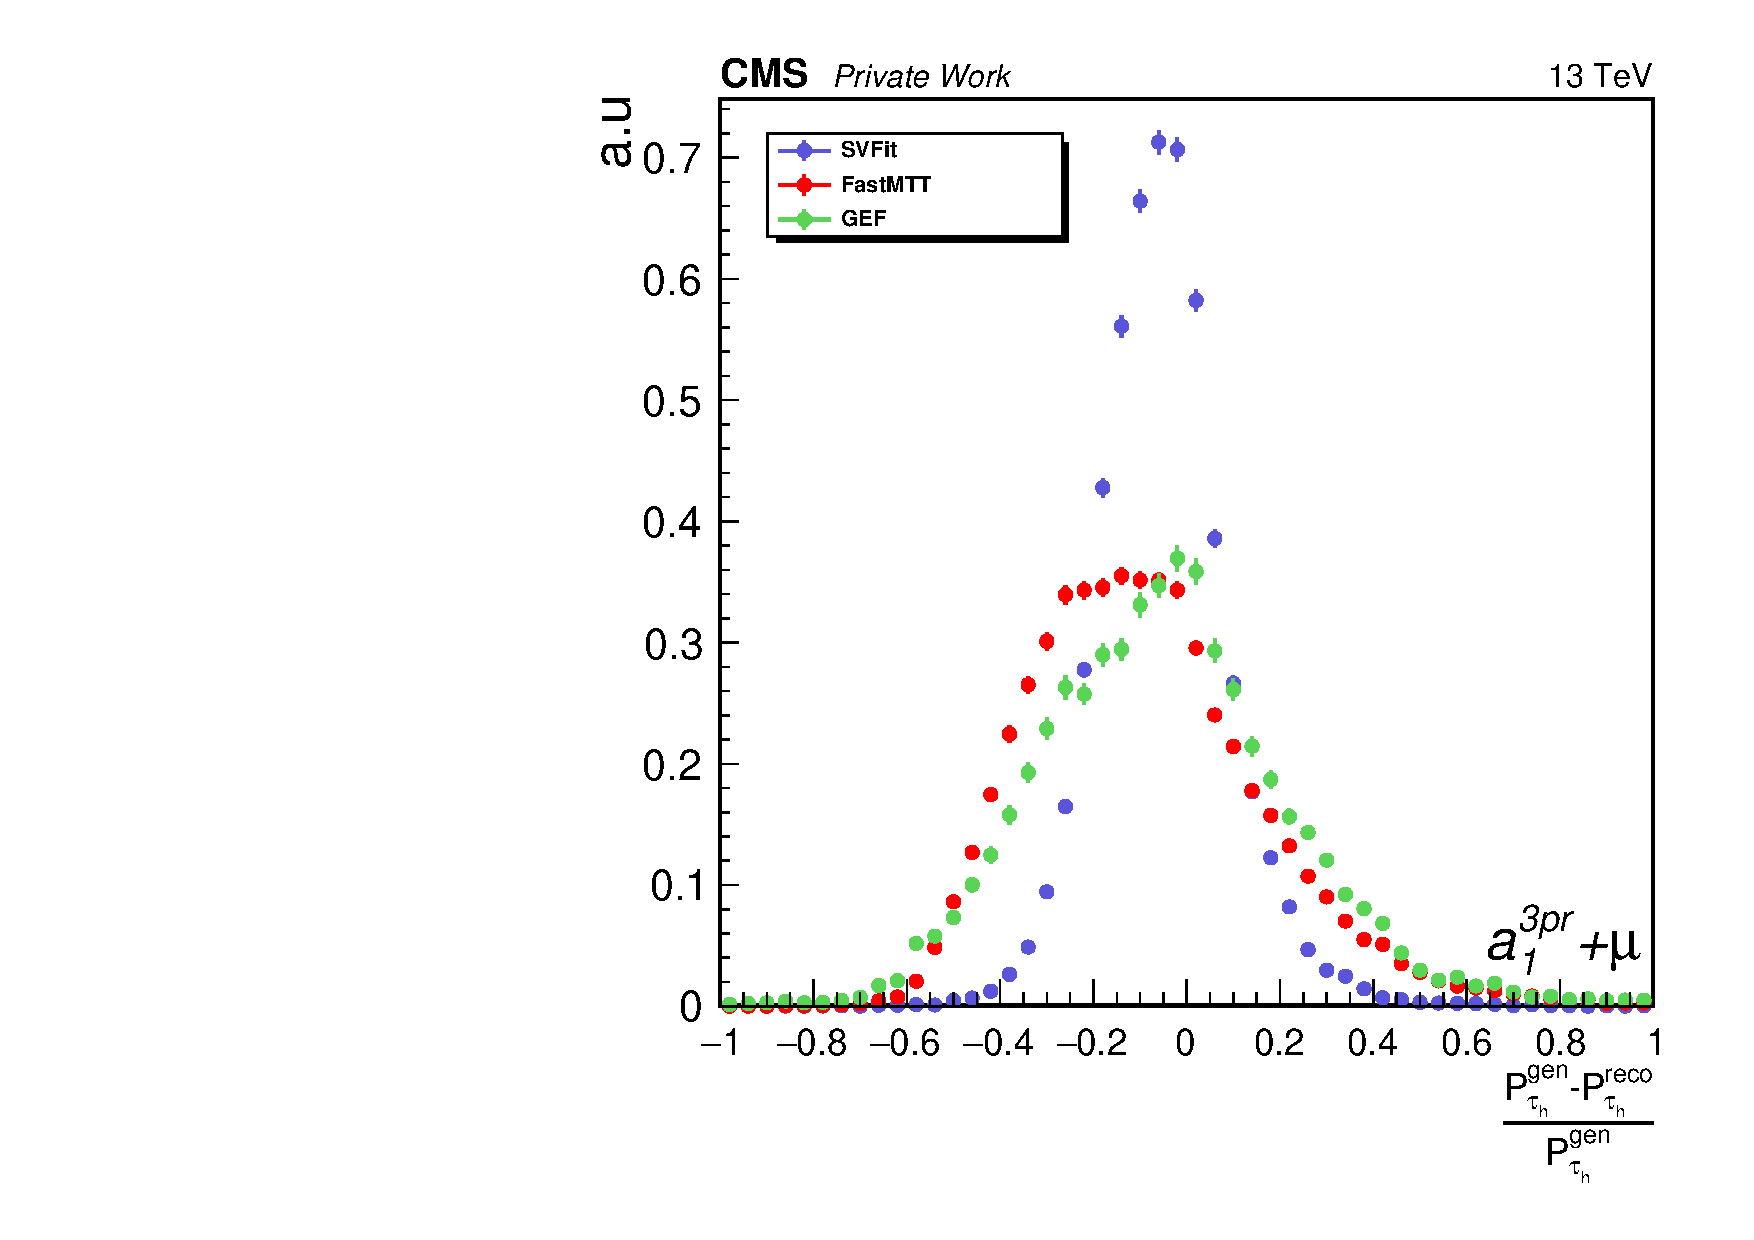
\includegraphics[width=\linewidth]{Chapitre6/Images/P.pdf} 
    \caption{} 
  \end{subfigure}%% 
  \begin{subfigure}[b]{0.5\linewidth}
    \centering
    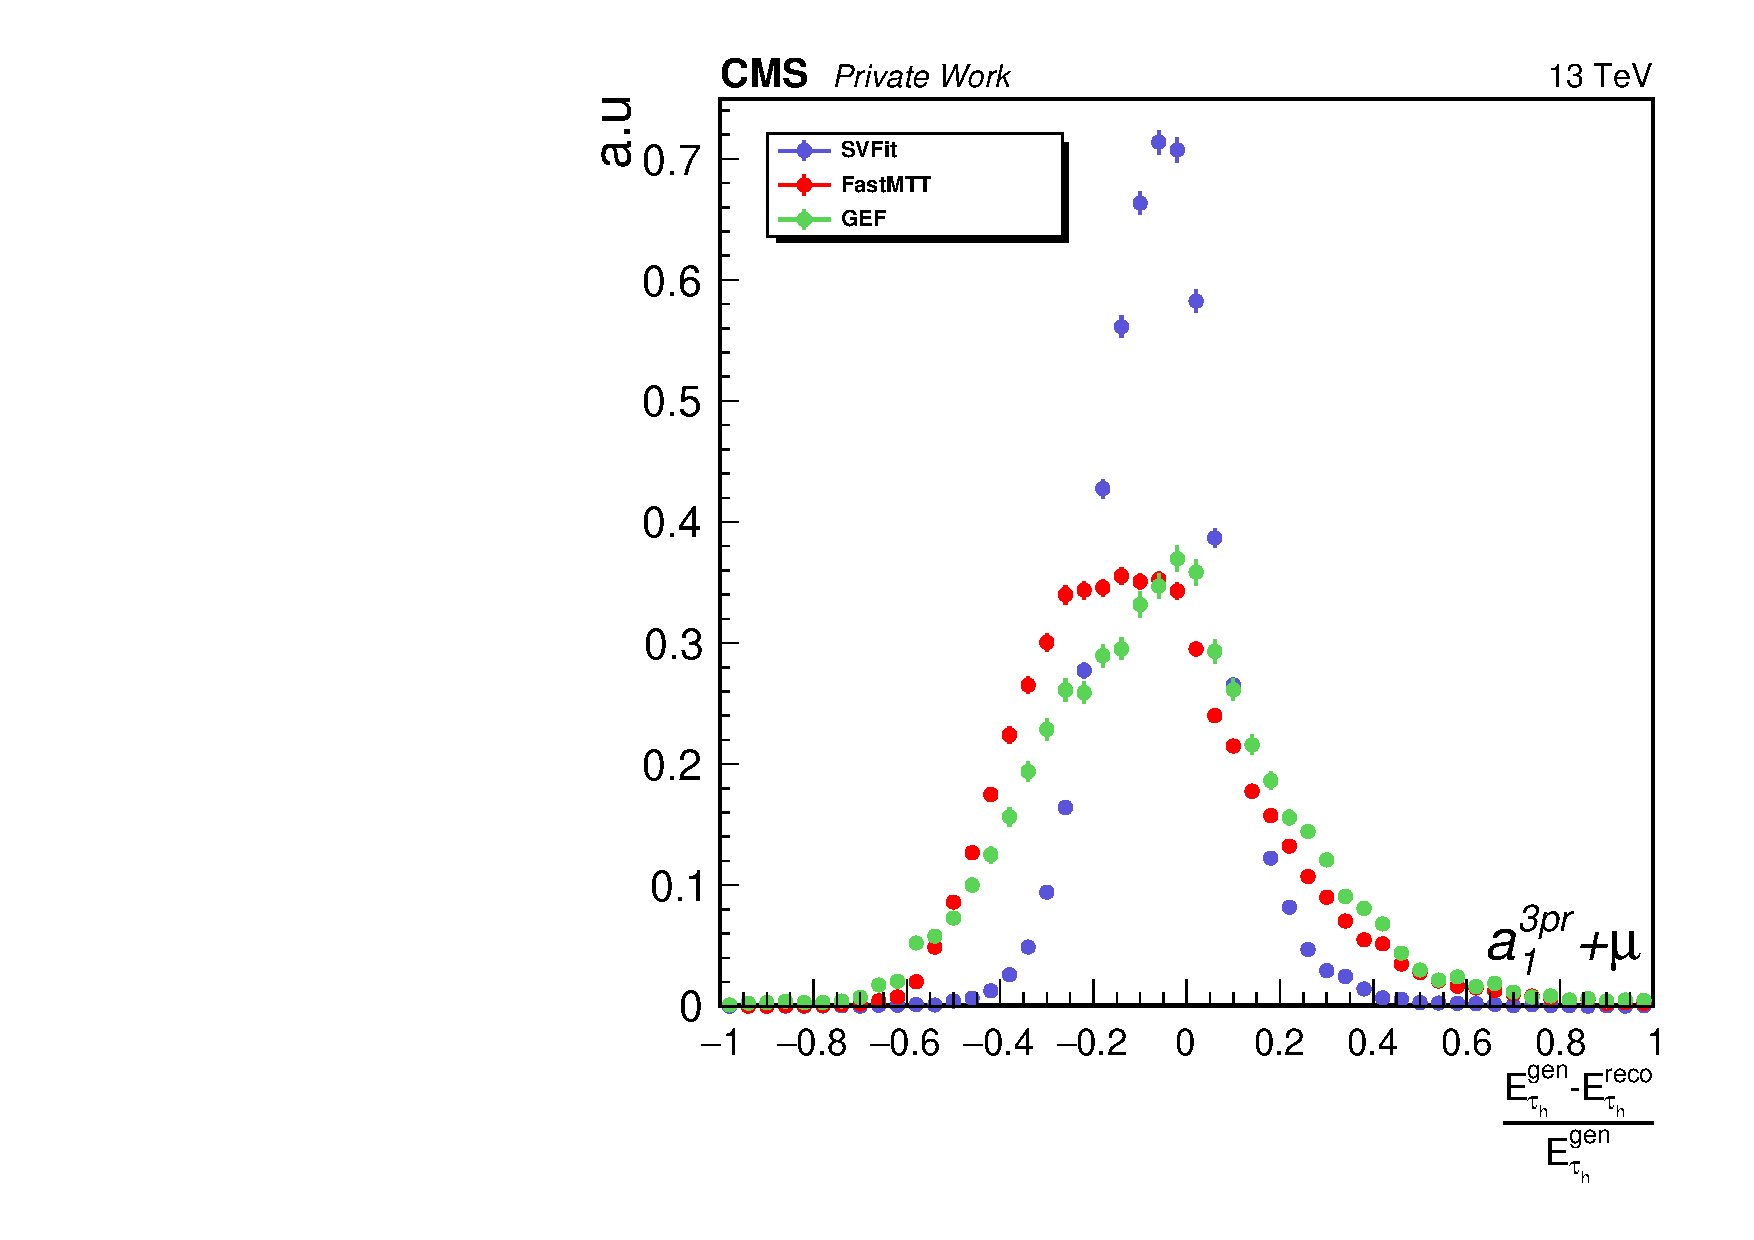
\includegraphics[width=\linewidth]{Chapitre6/Images/E.pdf} 
    \caption{} 
  \end{subfigure} 
  \caption{Résolution de reconstruction de $\eta$ (a), $\phi$ (b), la norme de l'impulsion (c) et l'énergie (d) du tau hadronique dans des évènements simulés $ggH\rightarrow\tau\tau$ dans le canal $a_1^{3pr}\mu$ avec l'algorithme SVFit (bleu), FastMTT (rouge) et GEF (vert).}
  \label{TauRes}
\end{figure}

La figure \ref{TauRes} présente la résolution de reconstruction des coordonnées du quadrivecteur du tau hadronique dans la désintégration $H\rightarrow\tau\tau$ dans l'état final $a_1\mu$. Les performances des trois algorithmes précédemment introduits sont comparées. On remarque notamment que l'algorithme SVFit possède la meilleure résolution en impulsion et en énergie mais la résolution angulaire la plus dégradée, tandis que GEF possède la meilleure résolution angulaire et une bonne résolution en énergie et impulsion.

\section{Variables optimales de spin du tau dans les samples \textit{embedded}}
\label{optvar}

L'étude suivante a été réalisée dans le cadre des EPR proposés par l'expérience CMS durant cette thèse. Comme pour toute désintégration, le spin du lepton tau est conservé sous la forme du moment angulaire total de ses produits de désintégration. Il possède cependant un intérêt expérimental particulier, puisque son spin est accessible à travers la mesure de plusieurs variables angulaires caractérisant sa désintégration. Le premier angle caractéristique est l'angle noté $\theta$ entre la direction du lepton tau et celle du hadron ou du lepton produit tel que vu dans le référentiel au repos du lepton tau. Dans le cas de la désintégration à deux corps $\tau^-\rightarrow\pi^-\nu_{\tau}$, seul le neutrino est porteur de spin et conserve celui du lepton tau. Un neutrino étant toujours d'hélicité gauche, cet effet entraîne une émission préférentielle du pion dans la direction du spin du lepton tau. Dans le référentiel au repos de ce dernier, le pion et le neutrino sont produits dans des directions opposées et ainsi dans le cas d'un tau d'hélicité gauche, le pion sera préférentiellement émis "vers l'avant" (i.e. $\cos(\theta)\approx 1$) et préférentiellement "vers l'arrière" (i.e. $\cos(\theta)\approx -1$) pour un tau d'hélicité droite. Ce mode de désintégration est toutefois le seul pour lequel toute l'information du spin est contenue dans l'angle $\theta$. Dans le cas d'une désintégration vers une résonance $\rho$ ou $a_1^{3pr}$ de spin 1, des angles supplémentaires dont la définition est donnée dans la figure \ref{angles} sont nécessaires à la description de la désintégration puisque ces dernières peuvent être polarisées de manière longitudinale ou transverse. \\

Pour un méson $\rho$, deux angles supplémentaires définis dans le référentiel au repos de la résonance sont considérés. Le premier, $\beta$, est défini entre la direction de la résonance $\rho$ et le pion chargé. Le second, $\alpha$, est défini entre le plan constitué par la direction du lepton tau et celle de la résonance $\rho$ et le plan constitué par la direction du pion chargé et celle de la résonance $\rho$. \\

Pour un méson $a_1^{3pr}$, un angle supplémentaire $\gamma$ est défini par l'orientation relative des trois pions chargés dans leur plan de désintégration. L'angle $\beta$ est défini cette fois entre la normale au plan constitué par les trois pions chargés et la direction de la résonance $a_1^{3pr}$. Tous les angles sont définis dans le référentiel au repos de la résonance $a_1^{3pr}$. \\

\begin{figure}[!ht]
    \centering
    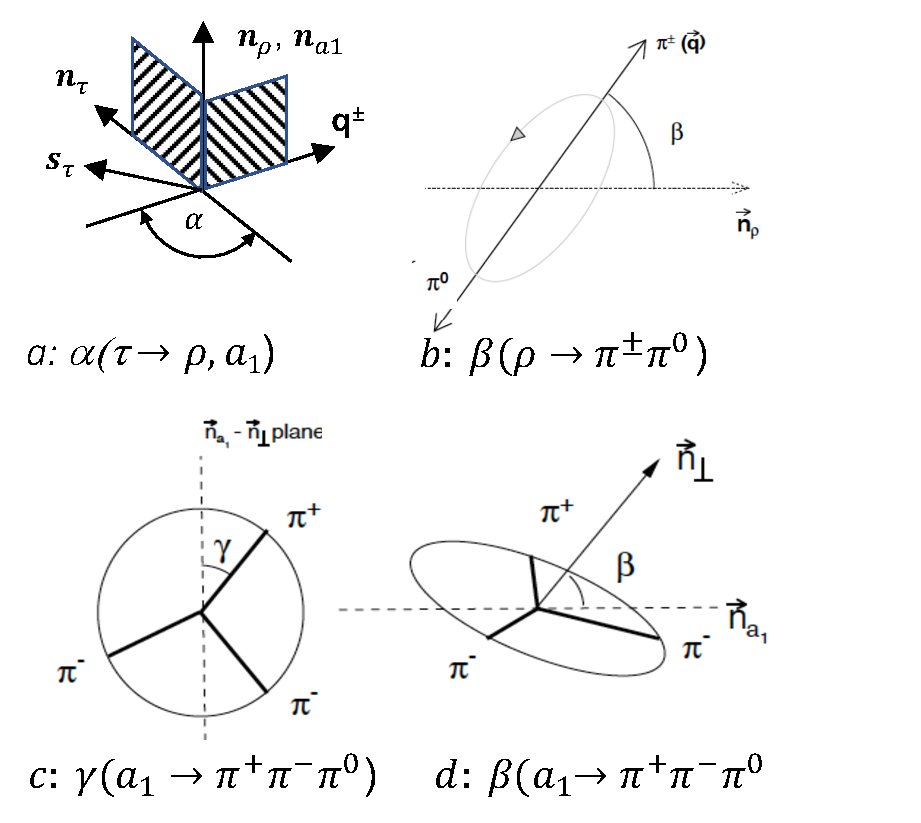
\includegraphics[scale=0.7]{Chapitre6/Images/angles.pdf}
    \caption{Définition de l'angle $\alpha$ dans les désintégrations $\tau_h\to\rho$ et $\tau_h\to a_1^{3pr}$ (a), de l'angle $\beta$ dans la désintégration $\tau_h\to\rho$ (b) et la désintégration $\tau_h\to a_1^{3pr}$ (d), et de l'angle $\gamma$ dans la désintégration $\tau_h\to a_1^{3pr}$ \cite{Zpol}.}
    \label{angles}
\end{figure}

La mesure de ces angles rentre notamment en jeu dans la mesure de la polarisation du lepton tau dans les désintégrations $Z\rightarrow\tau\tau$ \cite{Zpol}. Cette grandeur refléte l'asymétrie du couplage faible entre particules d'hélicité gauche et droite, et est directement reliée à l'angle de mélange électrofaible introduit dans la section \ref{EWK} du second chapitre. La section \ref{optvar} du chapitre \ref{analysis} sera dédiée à une introduction de variables de spin optimales construites à partir d'une combinaison des angles précédemment introduits et à une étude de leur distribution. D'autre part, l'étude de la structure CP des couplages de Yukawa étant elle aussi fondée sur l'information de spin, le lepton tau représente un candidat idéal dans cette tâche, contrairement au quark $b$ pour lequel cette information est perdue dans son mécanisme d'hadronisation malgré qu'il soit le mode de désintégration dominant du boson de Higgs.
D'après l'expression du taux de désintégration du lepton tau donnée dans l'équation \ref{dGamma} et telle que vue dans son référentiel au repos, la distribution angulaire du taux de désintégration peut s'exprimer sous la forme suivante :

\begin{equation}
    \frac{d\Gamma}{d\cos\theta_h}\propto\frac{1}{2}\bigl(1+P_{\tau}\cos\theta_h\bigr),
\end{equation}

\begin{figure}
    \begin{subfigure}[b]{0.5\linewidth}
    \centering
    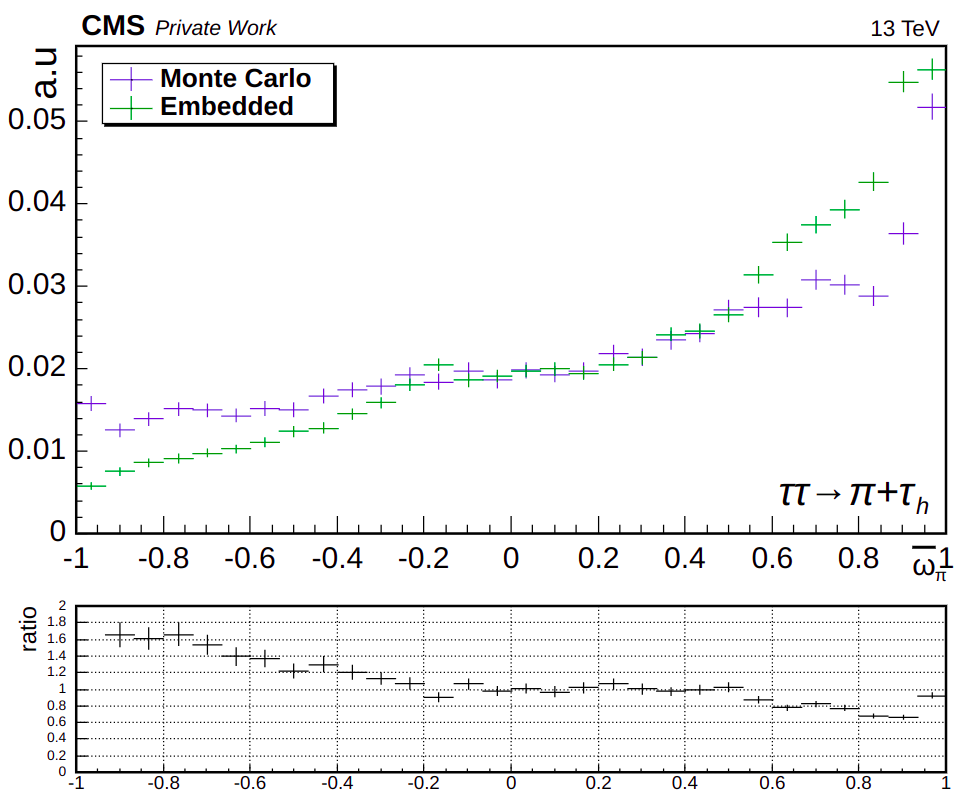
\includegraphics[width=\linewidth]{Chapitre6/Images/OptVar/omegabar_pi_pitauh.png} 
    \caption*{} 
    \vspace{10mm}
  \end{subfigure}%% 
  \begin{subfigure}[b]{0.5\linewidth}
    \centering
    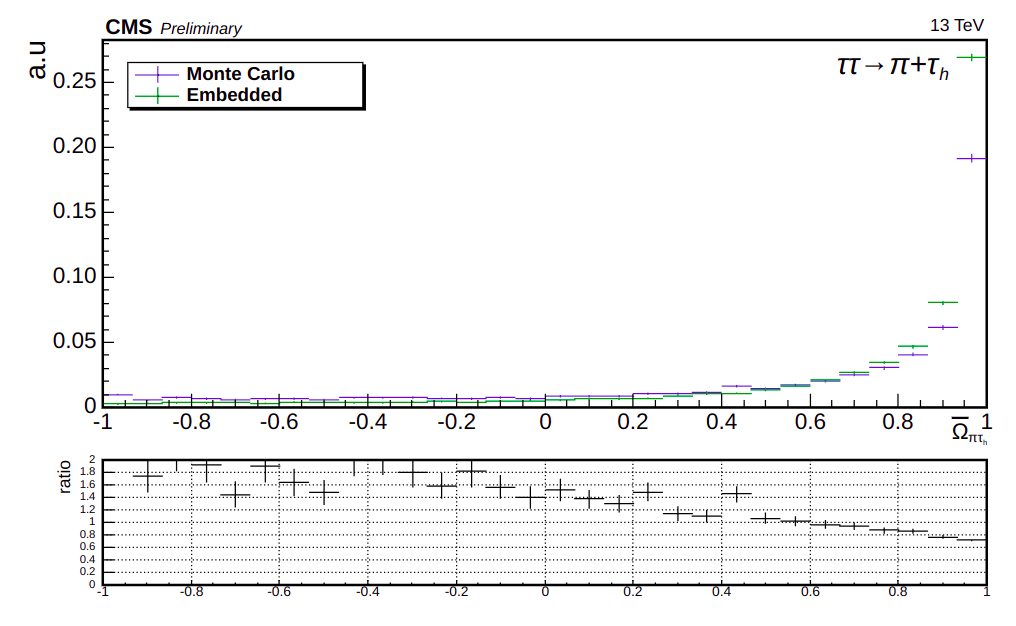
\includegraphics[width=\linewidth]{Chapitre6/Images/OptVar/Omegabar_pitauh.png} 
    \caption*{} 
    \vspace{10mm}
  \end{subfigure}
  %\vspace{30mm}
    \begin{subfigure}[b]{0.5\linewidth}
    \centering
    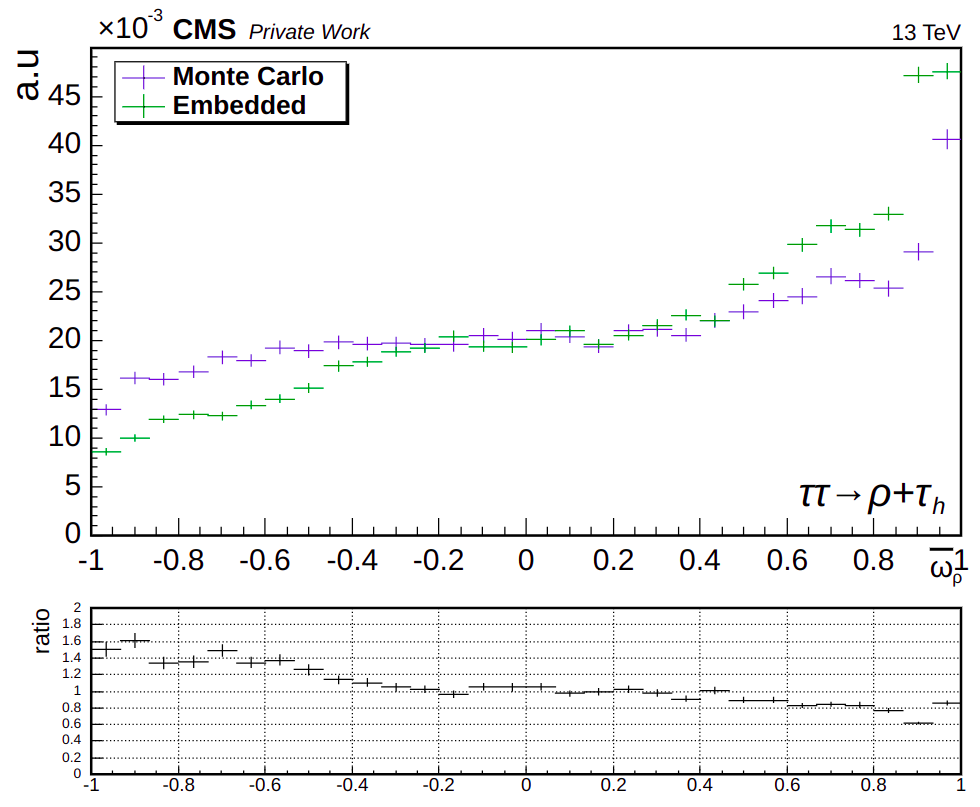
\includegraphics[width=\linewidth]{Chapitre6/Images/OptVar/omegabar_rho_rhotauh.png} 
    \caption*{} 
    \vspace{10mm}
  \end{subfigure}%% 
  \begin{subfigure}[b]{0.5\linewidth}
    \centering
    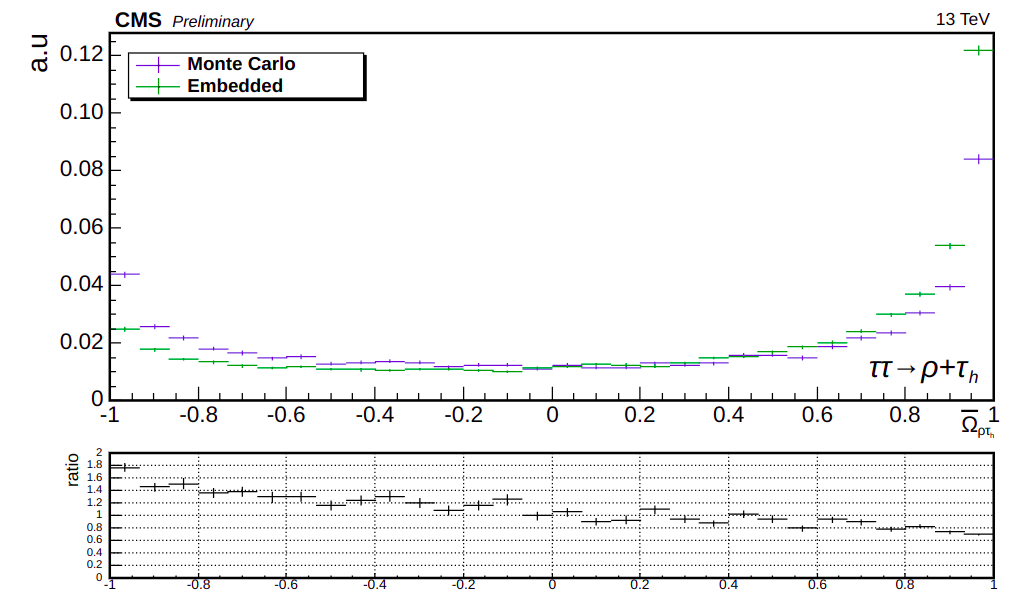
\includegraphics[width=\linewidth]{Chapitre6/Images/OptVar/Omegabar_rhotauh.png} 
    \caption*{} 
    \vspace{10mm}
  \end{subfigure}
      \begin{subfigure}[b]{0.5\linewidth}
    \centering
    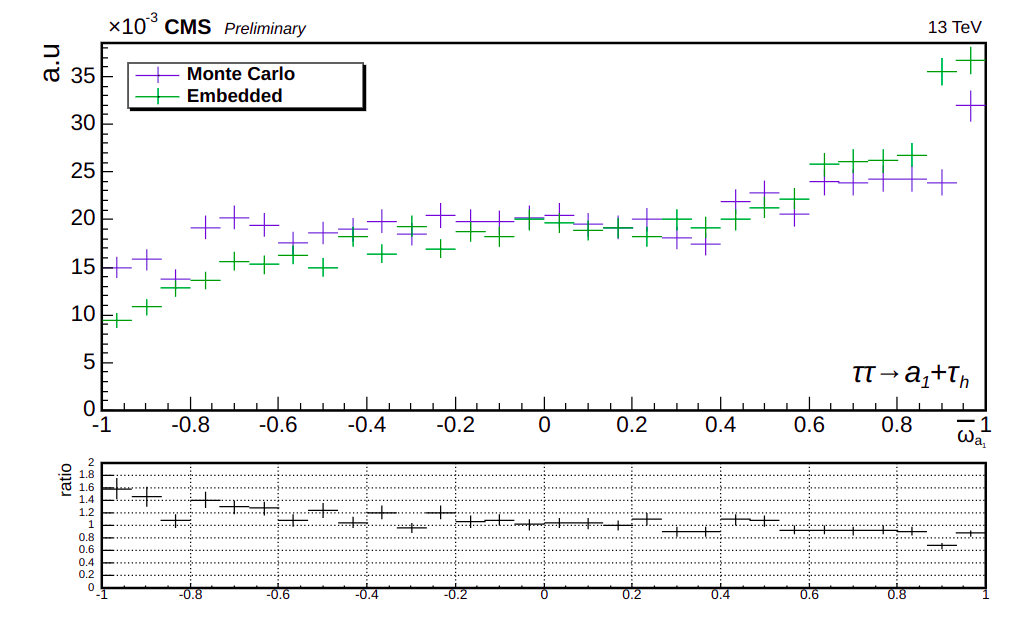
\includegraphics[width=\linewidth]{Chapitre6/Images/OptVar/omegabar_a1_a1tauh.png} 
    \caption*{} 
    \vspace{0.5ex}
  \end{subfigure}%% 
  \begin{subfigure}[b]{0.5\linewidth}
    \centering
    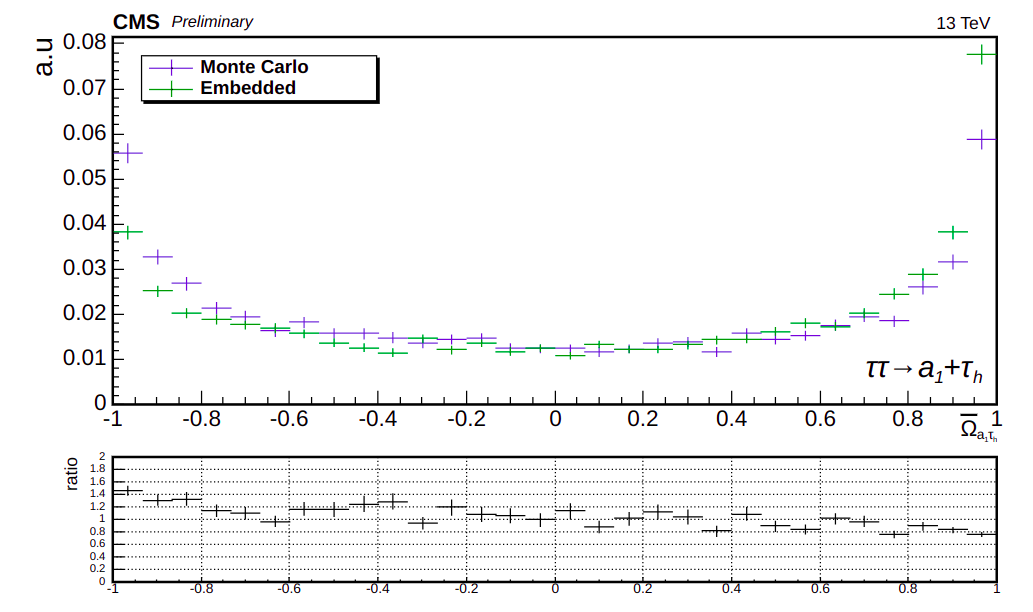
\includegraphics[width=\linewidth]{Chapitre6/Images/OptVar/Omegabar_a1tauh.png} 
    \caption*{} 
    \vspace{0.5ex}
  \end{subfigure}
  \caption{Comparaison de la distribution de $\overline{\omega}$ et $\overline{\Omega}$ dans les canaux $\pi\mu$ (haut), $\rho\mu$ (milieu) et $a_1^{3pr}\mu$ (bas) dans les échantillons Monte Carlo (violet) et embeddés (vert). Pour chaque canal, la variable $\overline{\omega}$ concerne uniquement le hadron spécifié.}
  \label{omegabar_tautau}
\end{figure}

\begin{figure}
    \begin{subfigure}[b]{0.5\linewidth}
    \centering
    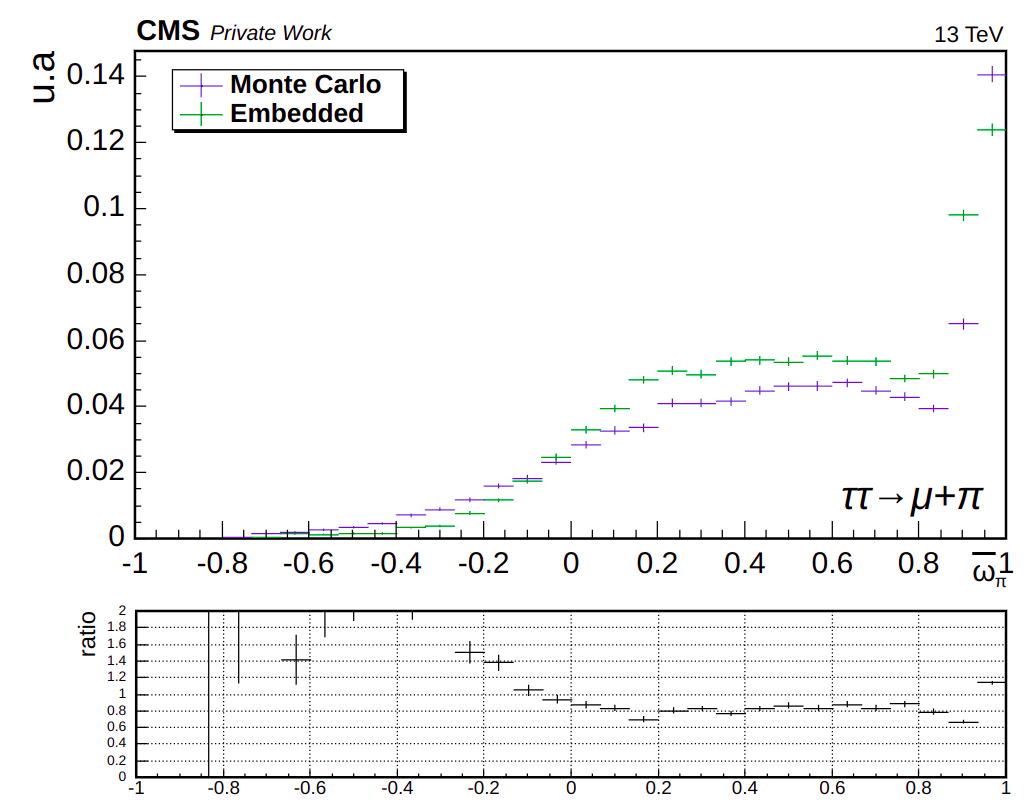
\includegraphics[width=\linewidth]{Chapitre6/Images/OptVar/omegabar_pi_pimu.png} 
    \caption*{} 
    \vspace{10mm}
  \end{subfigure}%% 
  \begin{subfigure}[b]{0.5\linewidth}
    \centering
    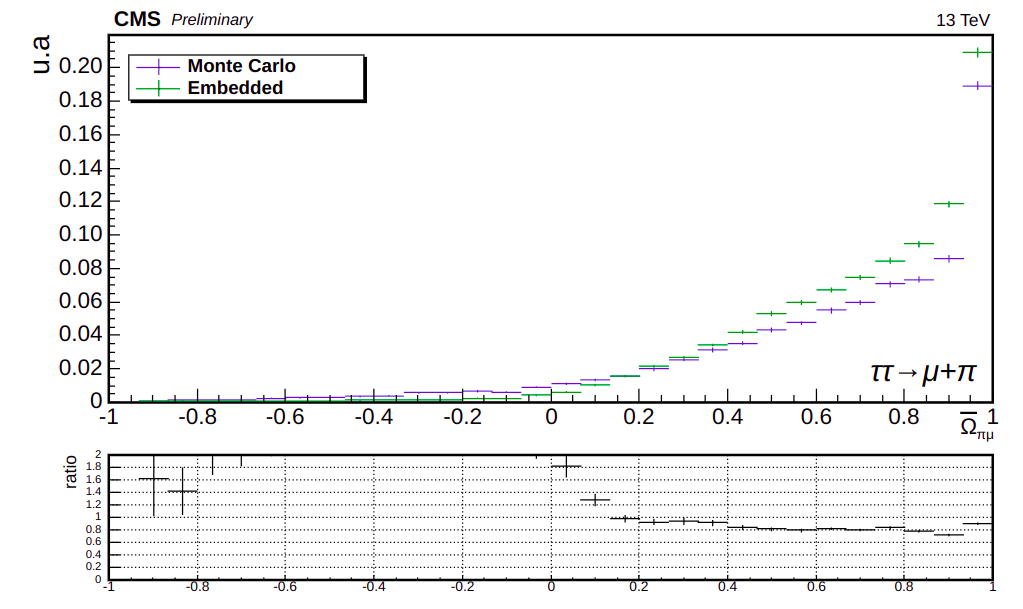
\includegraphics[width=\linewidth]{Chapitre6/Images/OptVar/Omegabar_pimu.png} 
    \caption*{} 
    \vspace{10mm}
  \end{subfigure}

    \begin{subfigure}[b]{0.5\linewidth}
    \centering
    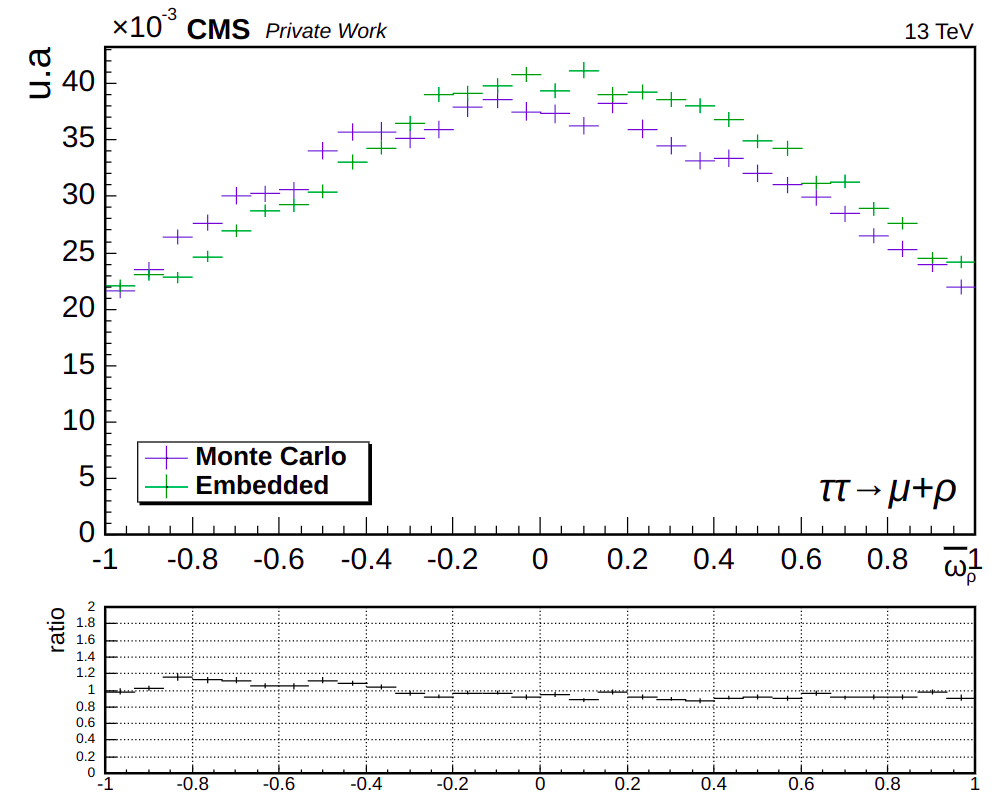
\includegraphics[width=\linewidth]{Chapitre6/Images/OptVar/omegabar_rho_rhomu.png} 
    \caption*{} 
    \vspace{10mm}
  \end{subfigure}%% 
  \begin{subfigure}[b]{0.5\linewidth}
    \centering
    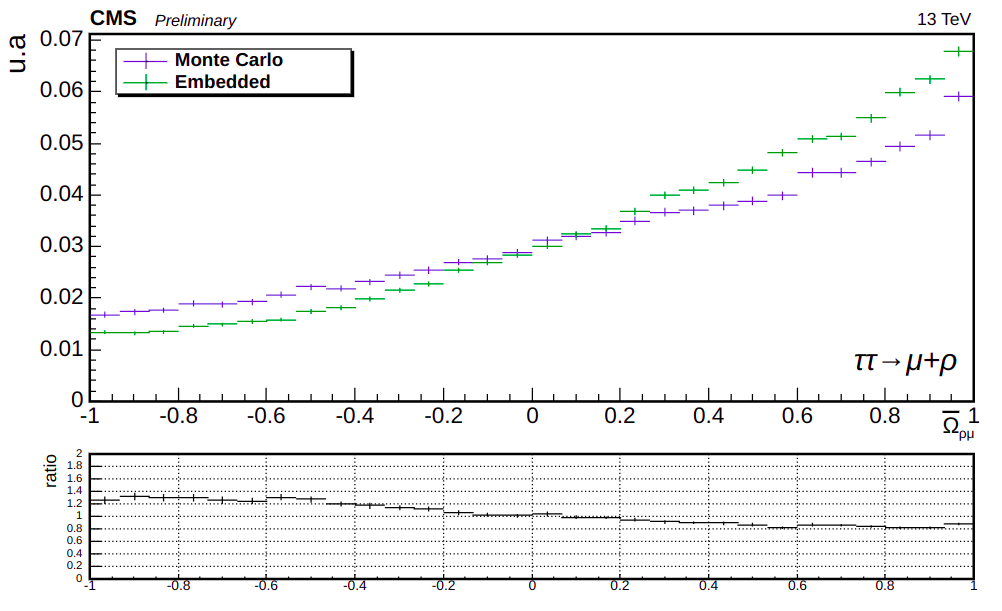
\includegraphics[width=\linewidth]{Chapitre6/Images/OptVar/Omegabar_rhomu.png} 
    \caption*{} 
    \vspace{10mm}
  \end{subfigure}
  
    \begin{subfigure}[b]{0.5\linewidth}
    \centering
    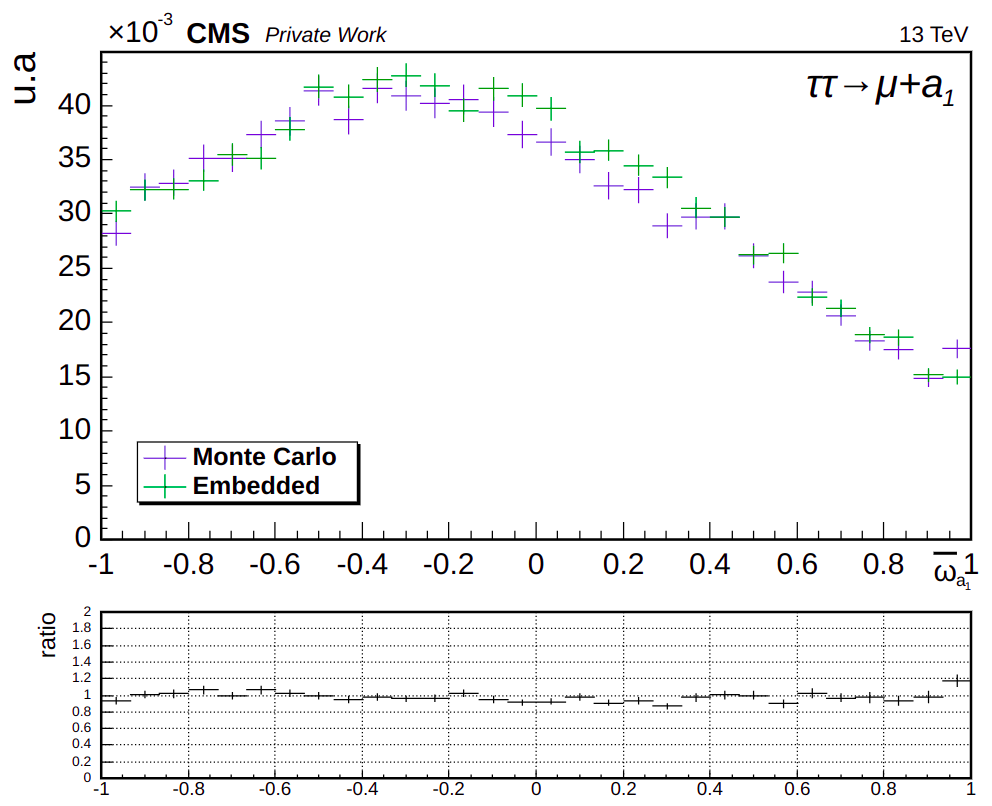
\includegraphics[width=\linewidth]{Chapitre6/Images/OptVar/omegabar_a1_a1mu.png} 
    \caption*{} 
    \vspace{0.5ex}
  \end{subfigure}%% 
  \begin{subfigure}[b]{0.5\linewidth}
    \centering
    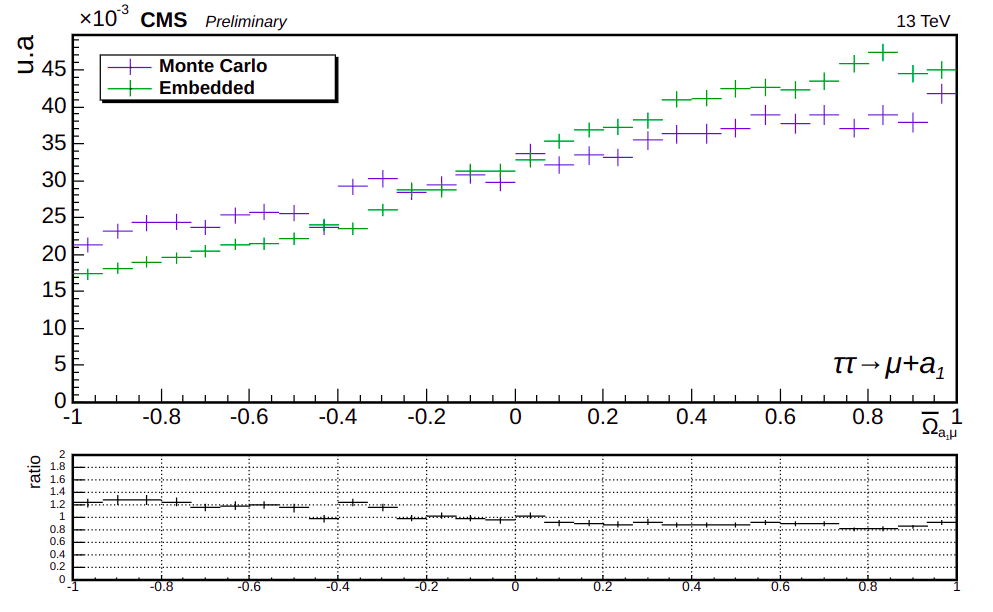
\includegraphics[width=\linewidth]{Chapitre6/Images/OptVar/Omegabar_a1mu.png} 
    \caption*{} 
    \vspace{0.5ex}
  \end{subfigure}
  \caption{Comparaison de la distribution de $\overline{\omega}$ et $\overline{\Omega}$ dans les canaux $\pi+\tau_h$ (haut), $\rho+\tau_h$ (milieu) et $a_1^{3pr}+\tau_h$ (bas) dans les échantillons Monte Carlo (violet) et embeddés (vert). Pour chaque canal, la variable $\overline{\omega}$ concerne uniquement le hadron spécifié.}
  \label{omegabar_mutau}
\end{figure}

\begin{figure}[!ht]
    \begin{subfigure}[b]{0.5\linewidth}
    \centering
    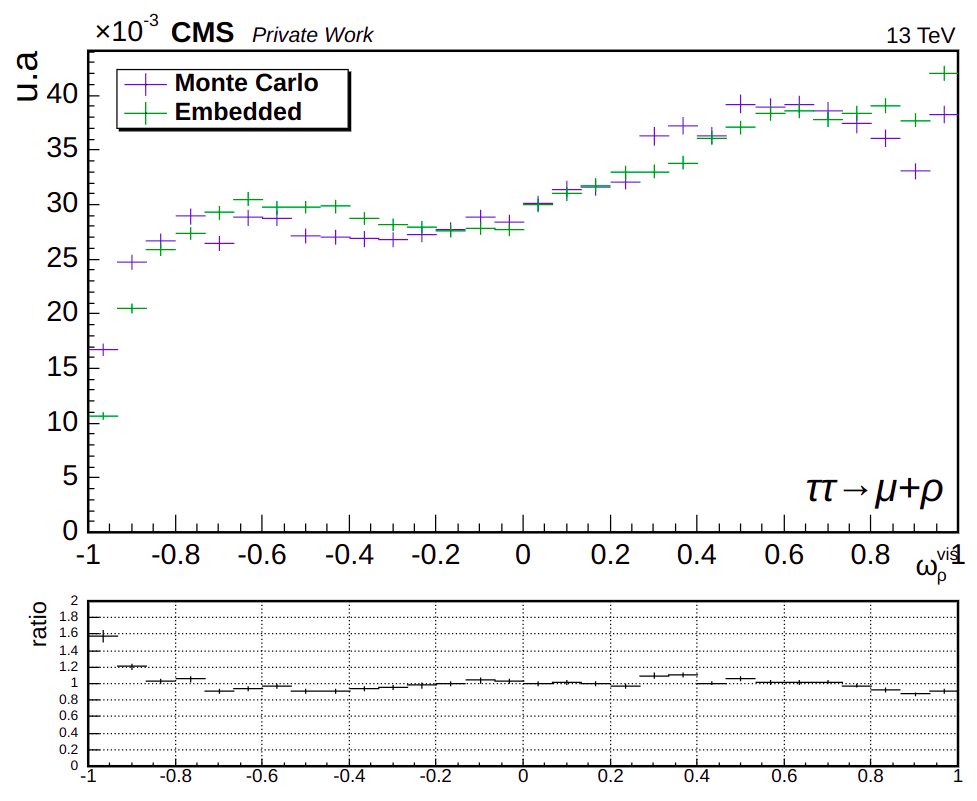
\includegraphics[width=\linewidth]{Chapitre6/Images/OptVar/omegavis_rho_rhomu.png} 
    \caption*{} 
    \vspace{0.5ex}
  \end{subfigure}%% 
  \begin{subfigure}[b]{0.5\linewidth}
    \centering
    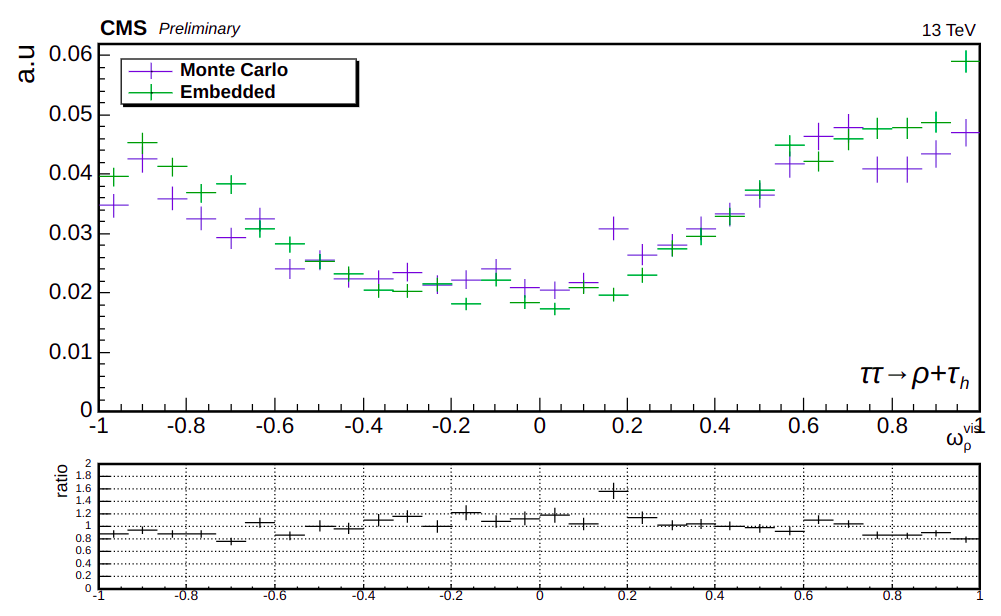
\includegraphics[width=\linewidth]{Chapitre6/Images/OptVar/omegavis_rho_rhotauh.png} 
    \caption*{} 
    \vspace{0.5ex}
  \end{subfigure}

    \begin{subfigure}[b]{0.5\linewidth}
    \centering
    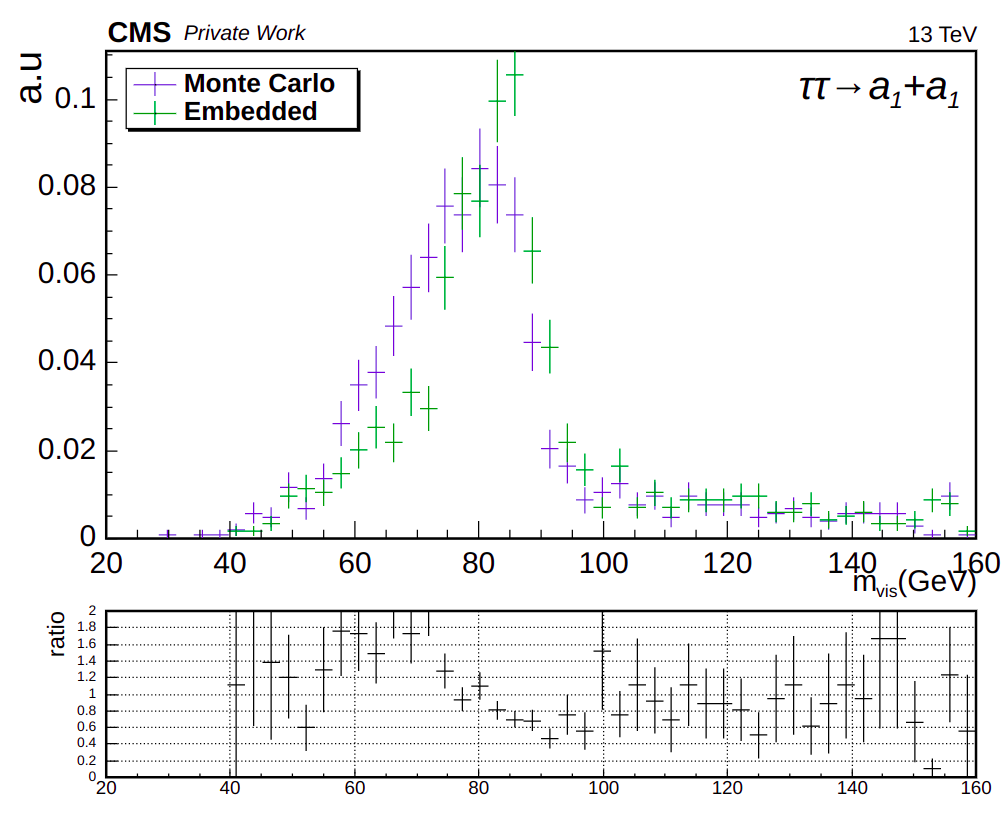
\includegraphics[width=\linewidth]{Chapitre6/Images/OptVar/mvis_a1a1.png} 
    \caption*{} 
    \vspace{0.5ex}
  \end{subfigure}%% 
  \begin{subfigure}[b]{0.5\linewidth}
    \centering
    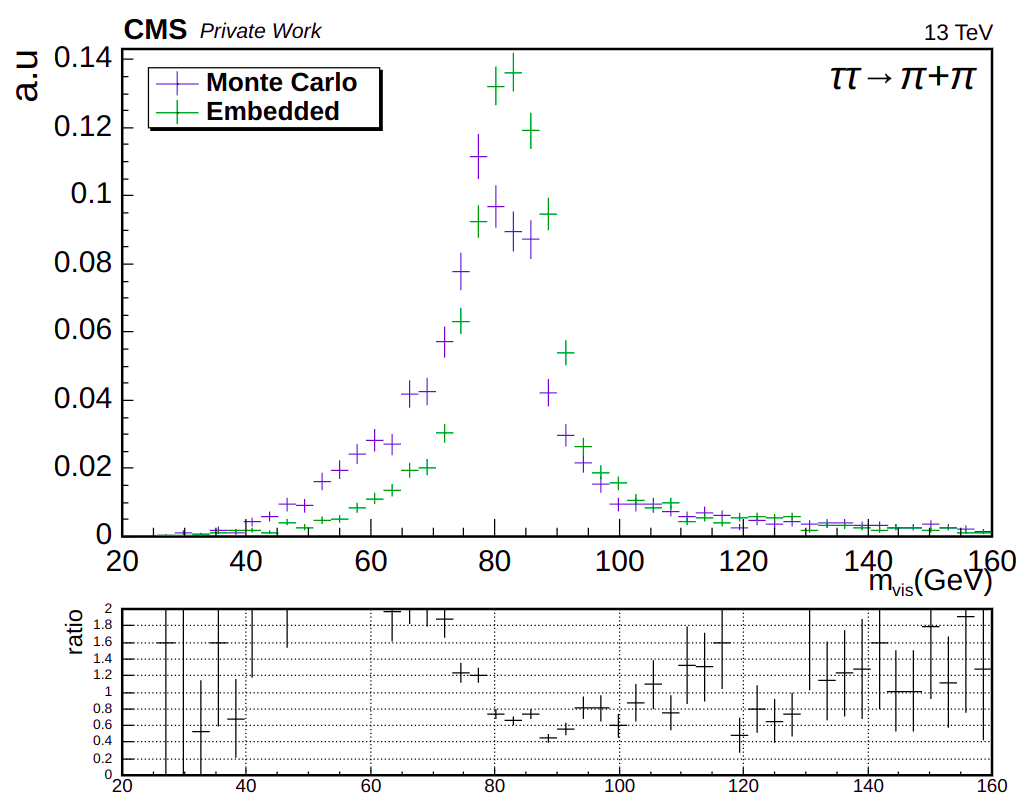
\includegraphics[width=\linewidth]{Chapitre6/Images/OptVar/mvis_pipi.png} 
    \caption*{} 
    \vspace{0.5ex}
  \end{subfigure}
  \caption{Comparaison de la distribution de $\overline{\omega}$ et $\overline{\Omega}$ dans les canaux $\pi+\tau_h$ (haut), $\rho+\tau_h$ (milieu) et $a_1^{3pr}+\tau_h$ (bas) dans les échantillons Monte Carlo (violet) et embeddés (vert). Pour chaque canal, la variable $\overline{\omega}$ concerne uniquement le hadron spécifié.}
  \label{optvarvis}
\end{figure}

où $\theta_h$ représente l'angle entre le vecteur polarimétrique et la direction du lepton tau et où $P_{\tau}$ représente sa polarisation moyenne ou son état d'hélicité pour une désintégration donnée. Dans le cas de la désintégration $\tau^-\rightarrow\pi^-\nu_{\tau}$, le vecteur polarimétrique est donné par la direction du neutrino et ainsi toute l'information sur l'état d'hélicité est contenue dans la variable $\theta$ définie dans la section \ref{tau properties} de sorte que $\cos\theta_h=-\cos\theta$. De la même façon, une variable optimale $\overline{\omega}$ peut être construite pour chaque mode de désintégration à partir des variables angulaires qui le caractérise et du vecteur polarimétrique telle que 

$$\overline{\omega}=\cos\theta_h.$$

Il est également possible d'exploiter l'anti-corrélation de l'hélicité des leptons tau au sein d'une paire afin de définir une variable optimale globale. Cette nouvelle variable tient compte de la variable optimale de chaque tau $\overline{\omega}_1$ et $\overline{\omega}_2$ et s'écrit :

\begin{equation}
    \overline{\Omega}=\frac{\overline{\omega}_1+\overline{\omega}_2}{1+\overline{\omega}_1\cdot\overline{\omega}_2}.
\end{equation}

La figure \ref{omegabar_tautau} présente une comparaison de la distribution des variables $\overline{\omega}$ et $\overline{\Omega}$ entre un échantillon Monte Carlo et un échantillon \textit{embedded}. Trois canaux sont étudiés : $\pi\tau_h$, $\rho\tau_h$, $a_1^{3pr}\tau_h$. Pour chaque canal, la variable $\overline{\omega}$ est définie pour le lepton tau dont le mode désintégration est spécifié ($\pi,\rho,a_1^{3pr}$). De manière générale, les distributions sont en bon accord, à l'exception de quelques désaccords de l'ordre de $10$ à $15\%$, principalement aux valeurs limites. Ces désaccords peuvent notamment être entraînés par des erreurs d'alignement entre la géométrie du détecteur réelle et celle du détecteur simulé dans laquelle la paire de leptons tau \textit{embedded} est produite. La figure \ref{omegabar_mutau} présente les mêmes distributions dans les canaux $\pi\mu$, $\rho\mu$, $a_1^{3pr}\mu$. La figure \ref{optvarvis} présente également les distributions de quelques variables utilisées dans la mesure de la polarisation du lepton tau \cite{Zpol} dans le cas où ces dernières possèdent un meilleur pouvoir discriminant que les variables optimales présentées précédemment. En particulier, dans les canaux impliquant une résonance $rho$ ($\rho\mu$, $\rho\tau_h$), la variable optimale $\omega_{\text{vis}}$ s'appuyant uniquement sur les produits de désintégration visibles est utilisée. Dans les canaux $a_1a_1$ et $\pi\pi$, la masse invariante visible $m_{\text{vis}}$ est utilisée.
    
\section{Performances du vecteur polarimétrique dans les canaux hadroniques} 
\label{perf}

Cette section est dédiée à l'étude des performances du vecteur polarimétrique face aux méthodes du pion neutre et du paramètre d'impact fondées uniquement sur les produits de désintégration visibles du lepton tau. Afin de comparer la sensibilité d'une méthode à une autre, la distribution de $\phi_{CP}$ pour chacune d'elle est ajustée par une fonction cosinus avec deux paramètres $a$ et $b$ telle que $f = a\cos(\phi_{CP})+b$. Le ratio $a/b$ de ces paramètres permet alors de quantifier l'amplitude de l'oscillation de la distribution de $\phi_{CP}$, un plus grand ratio offrant un meilleur pouvoir de séparation entre les différents états CP et donc une meilleure sensibilité. Les performances du vecteur polarimétrique sont évaluées dans les six canaux hadroniques $\tau_h\tau_h\rightarrow\pi\pi,\pi\rho,\rho\rho,a_1^{3pr}\pi,a_1^{3pr}\rho,a_1^{3pr}a_1^{3pr}$. Dans un premier temps une étude au niveau générateur est effectuée afin d'étudier les canaux les plus sujets à une amélioration de la sensibilité. Dans chaque figure présentée dans la suite, la distribution de $\phi_{CP}$ obtenue avec le vecteur polarimétrique (\textit{pol. vec.}) est comparée à celle obtenue avec la méthode du pion neutre (\textit{neutral pion}, NP) ou du paramètre d'impact (\textit{impact par.}, IP) en accord avec le canal considéré. Pour rappel, tandis que le vecteur polarimétrique est applicable à tous les canaux hadroniques, la méthode du paramètre d'impact est choisie pour l'état final $\tau_h\rightarrow\pi$ et la méthode du pion neutre pour les états finaux $\tau_h\rightarrow\rho,a_1^{3pr}$. Dans le cas des canaux $\tau_h\tau_h\rightarrow a_1^{3pr}\rho,a_1^{3pr}\pi$, il est alors possible d'appliquer la méthode du vecteur polarimétrique sur les deux états finaux ou de conserver l'utilisation du paramètre d'impact sur l'état final $\tau_h\rightarrow\pi$ et de n'appliquer le vecteur polarimétrique que sur la résonance $\rho$ ou $a_1^{3pr}$. \\

\begin{figure}[]
  \begin{subfigure}[b]{0.5\linewidth}
    \centering
    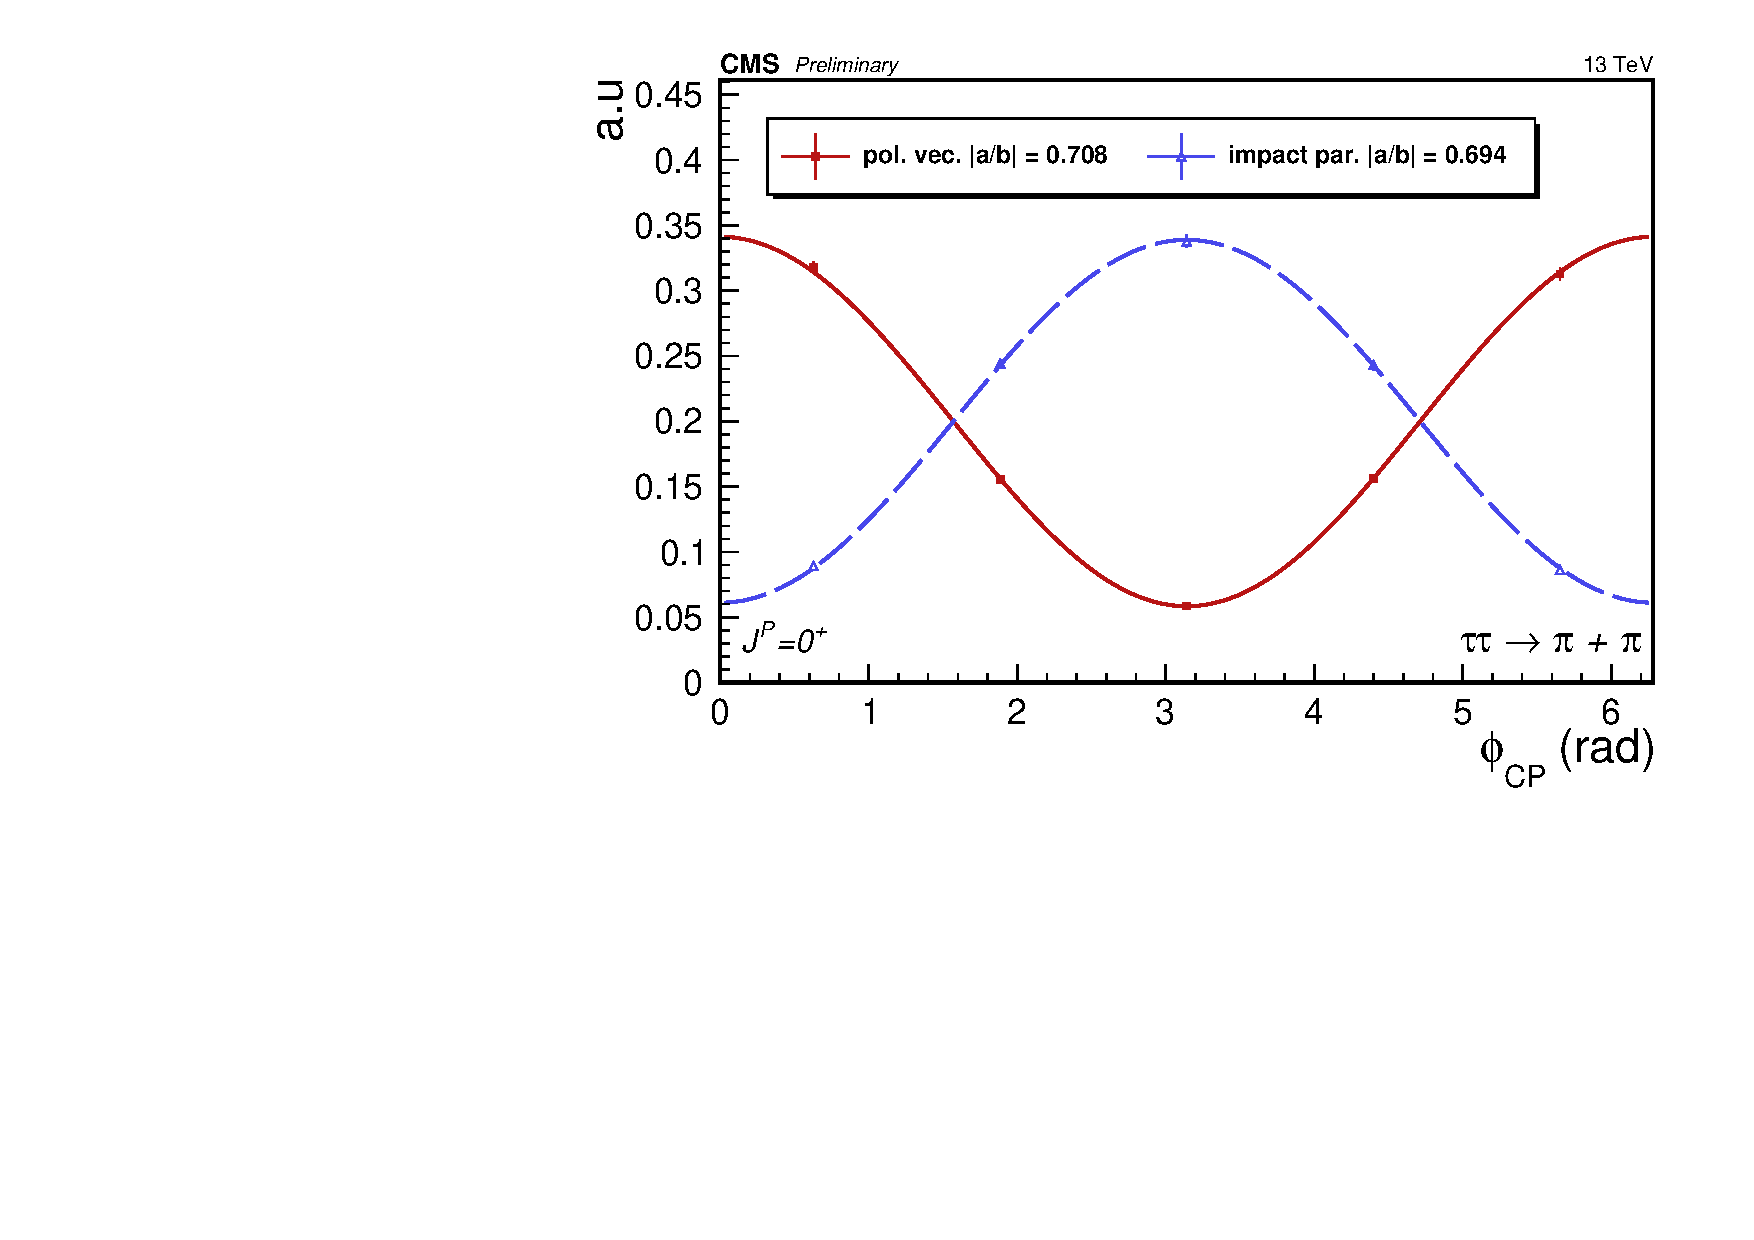
\includegraphics[width=\linewidth]{Chapitre6/Images/PIONPION/PIONPION_even_gen.pdf} 
    \caption*{} 
    \vspace{0.5ex}
  \end{subfigure}%% 
  \begin{subfigure}[b]{0.5\linewidth}
    \centering
    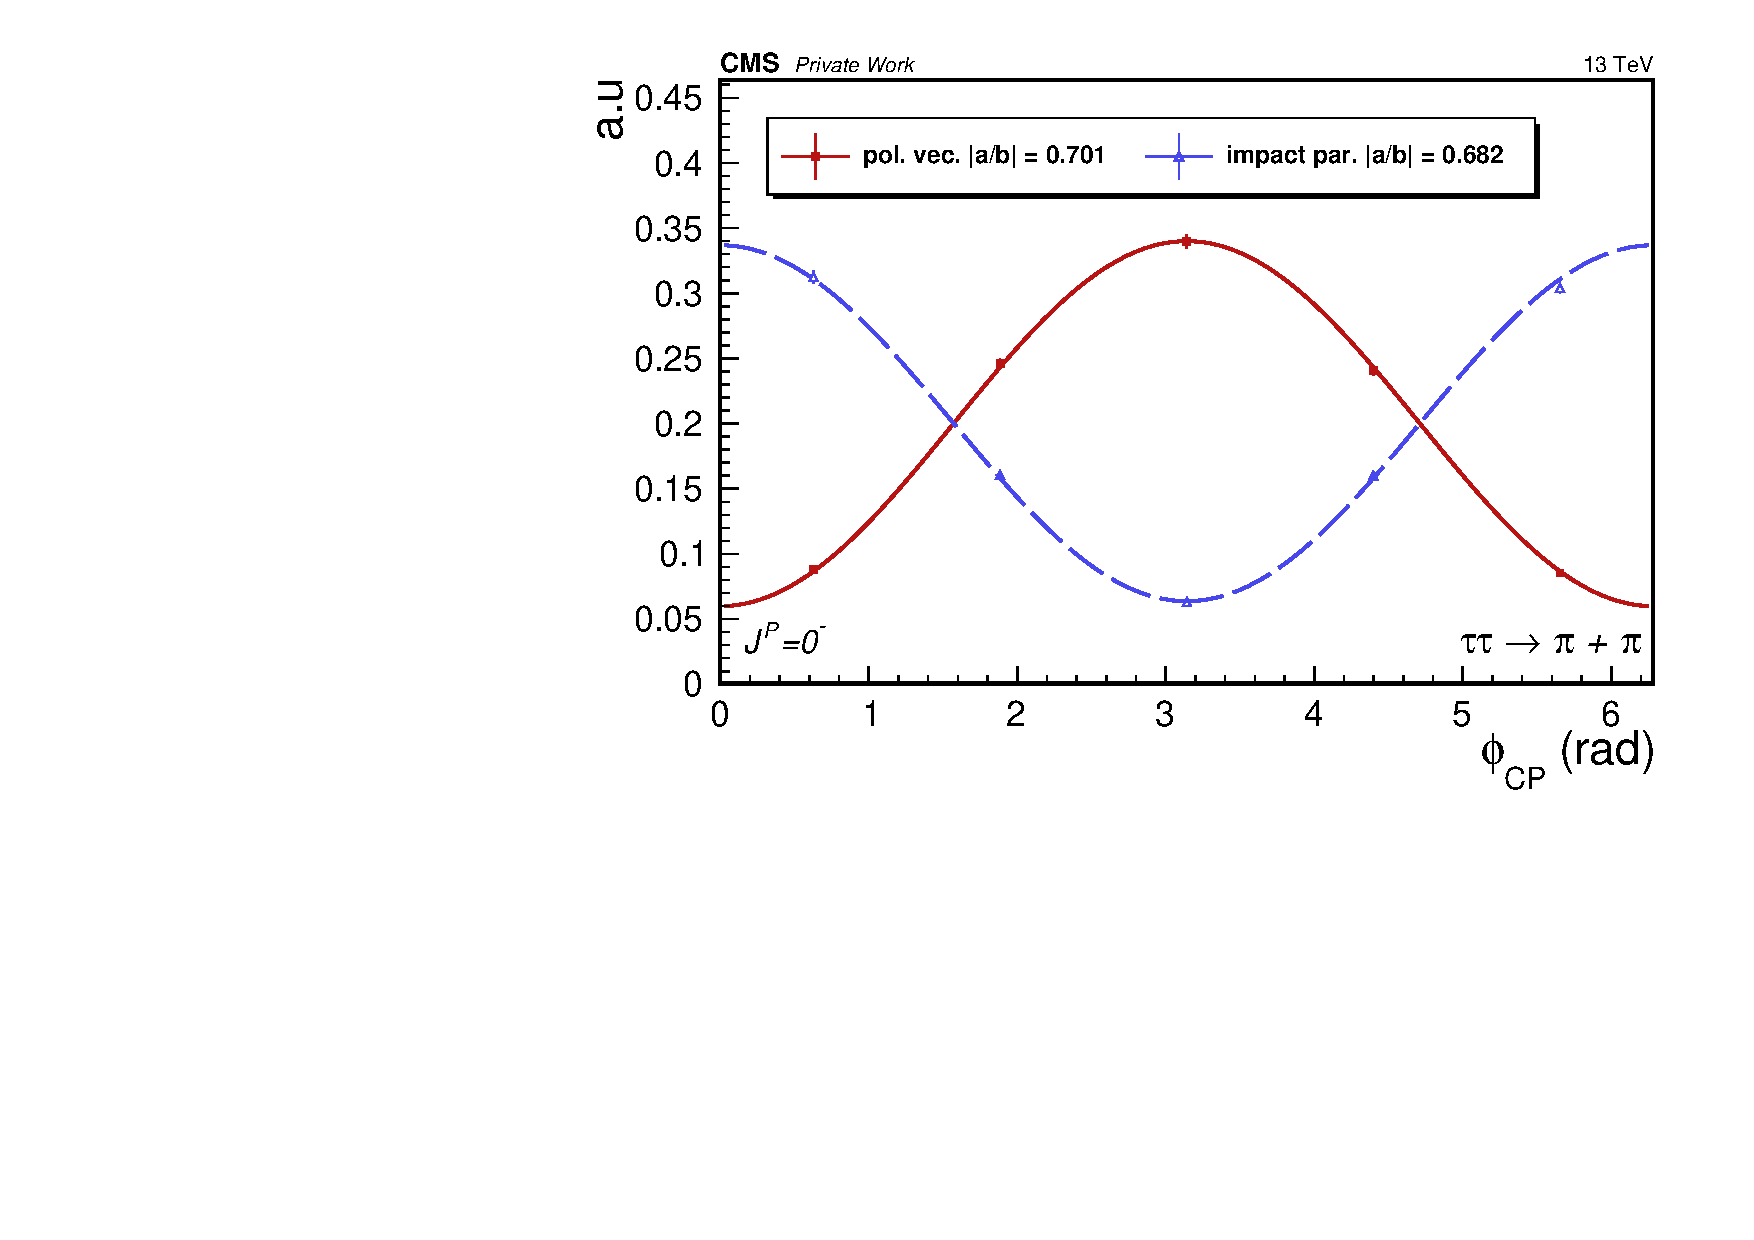
\includegraphics[width=\linewidth]{Chapitre6/Images/PIONPION/PIONPION_odd_gen.pdf} 
    \caption*{} 
    \vspace{0.5ex}
  \end{subfigure} 
  \caption{Distribution de $\phi_{CP}$ dans le canal $\tau_h\tau_h\rightarrow\pi\pi$ au niveau générateur pour l'état CP pair (gauche) et CP impair (droite) dans des évènements $ggH\to\tau\tau$.}
  \label{CPgenPIPI}
\end{figure}


\begin{figure}[]
  \begin{subfigure}[b]{0.5\linewidth}
    \centering
    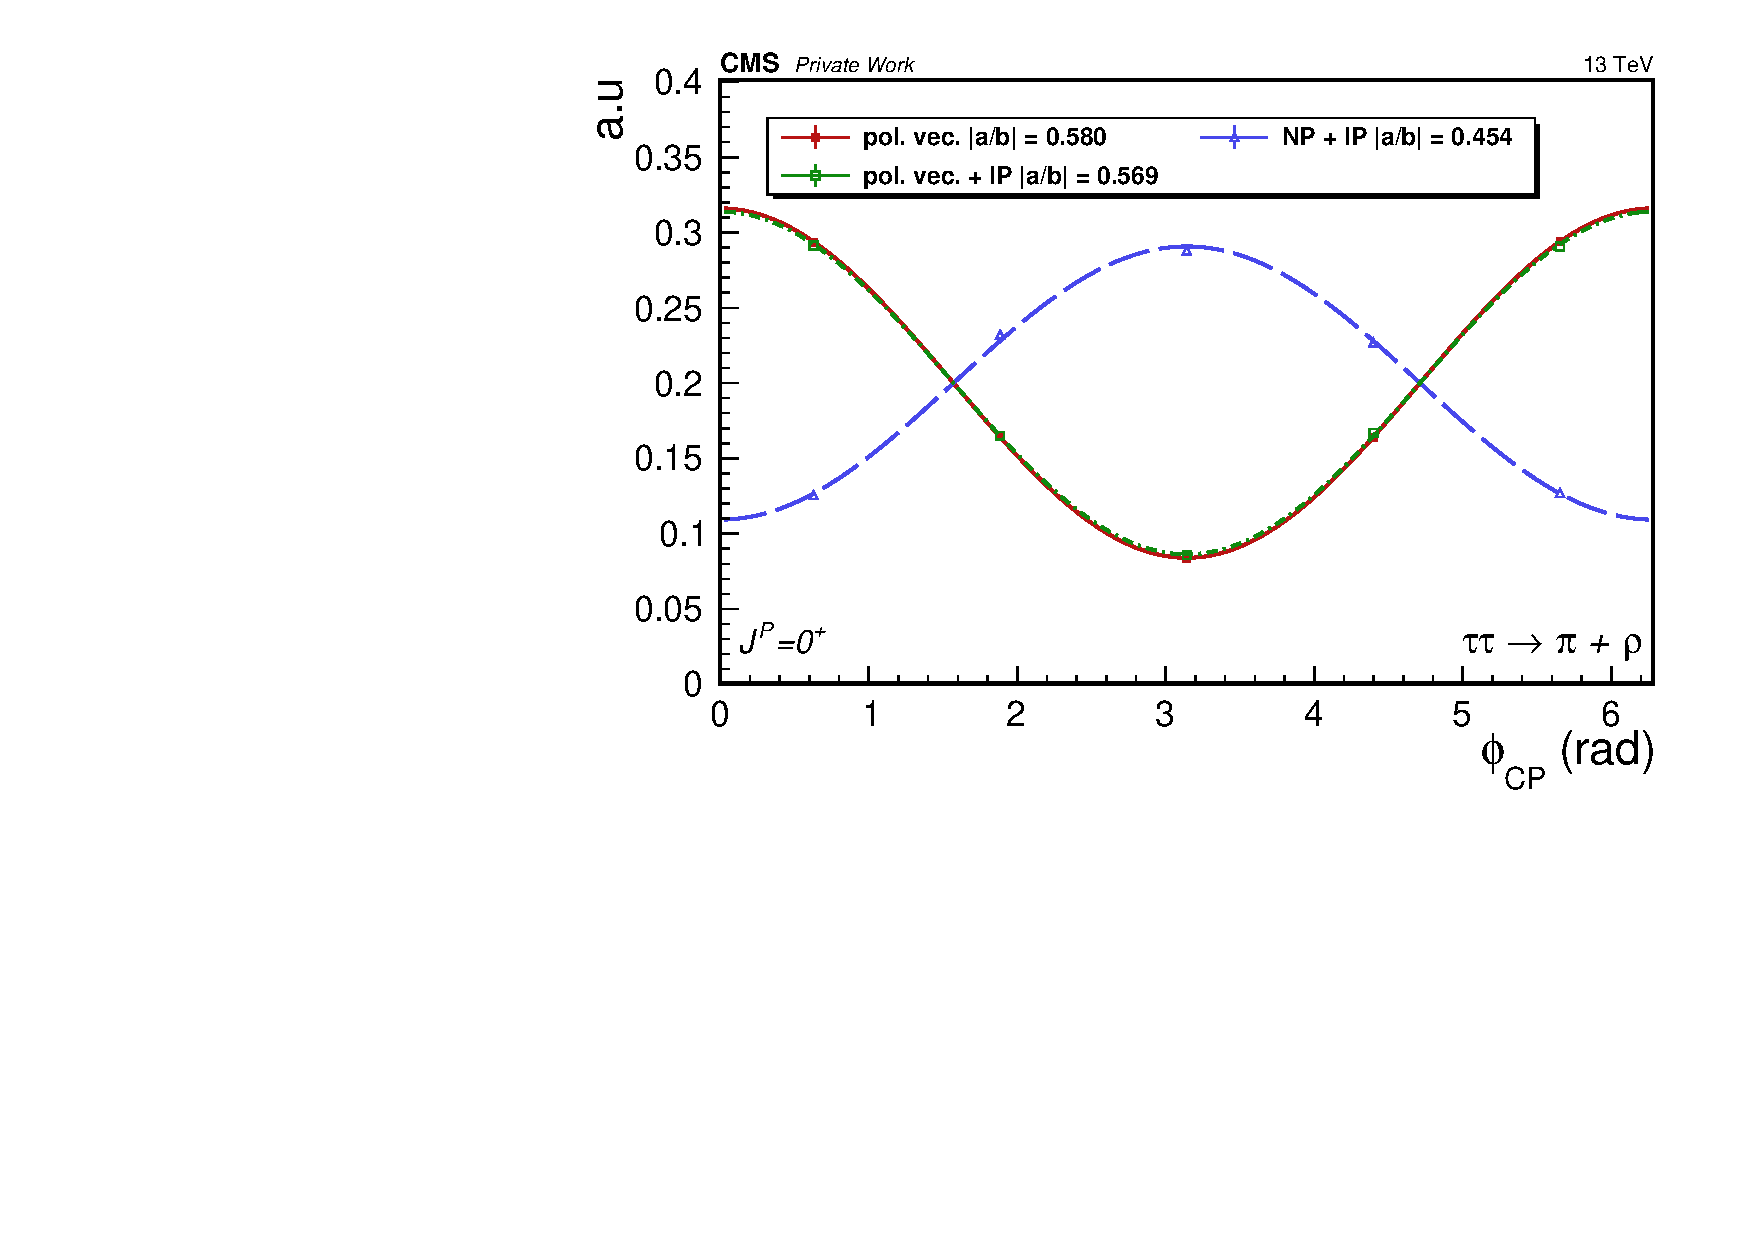
\includegraphics[width=\linewidth]{Chapitre6/Images/RHOPION/RHOPION_even_gen.pdf} 
    \caption*{} 
    \vspace{10mm}
  \end{subfigure}%% 
  \begin{subfigure}[b]{0.5\linewidth}
    \centering
    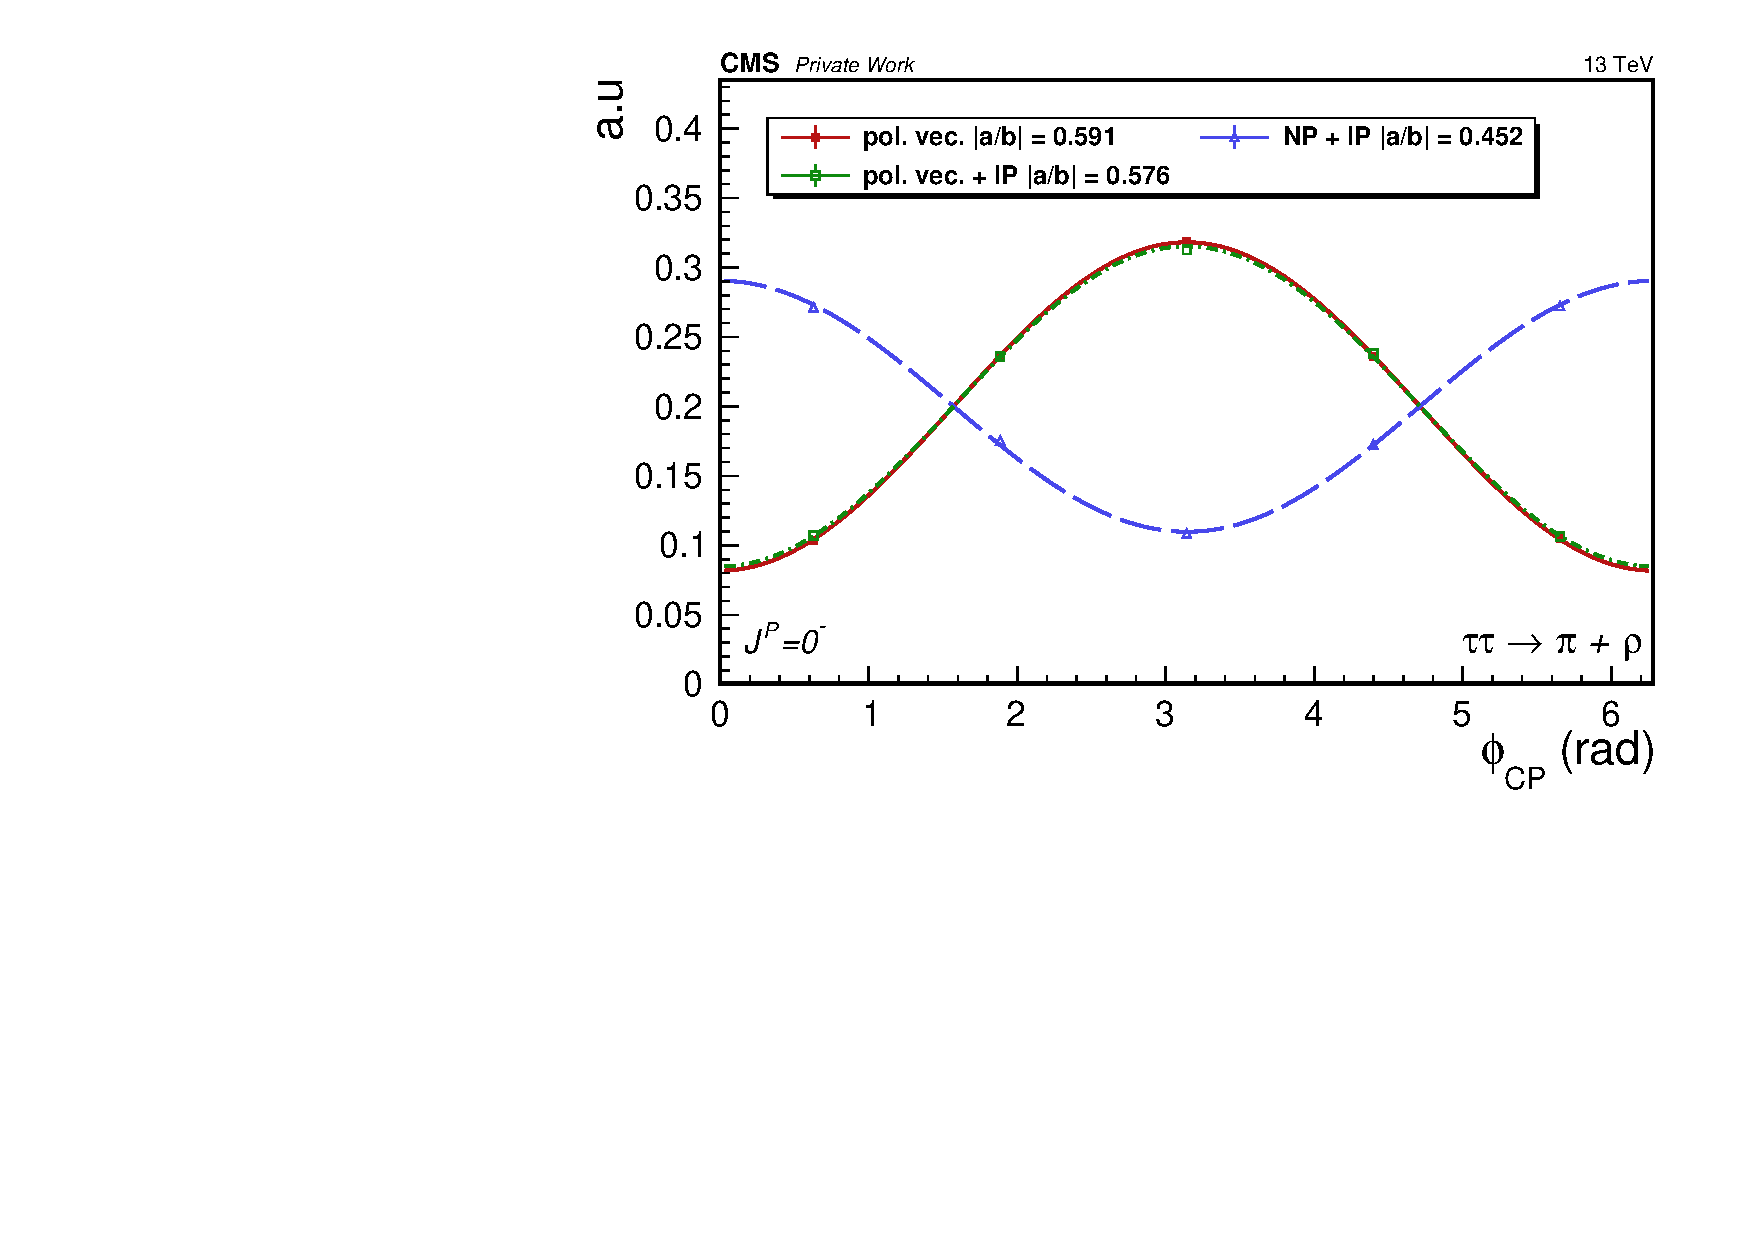
\includegraphics[width=\linewidth]{Chapitre6/Images/RHOPION/RHOPION_odd_gen.pdf} 
    \caption*{} 
    \vspace{10mm}
  \end{subfigure} 

  \begin{subfigure}[b]{0.5\linewidth}
    \centering
    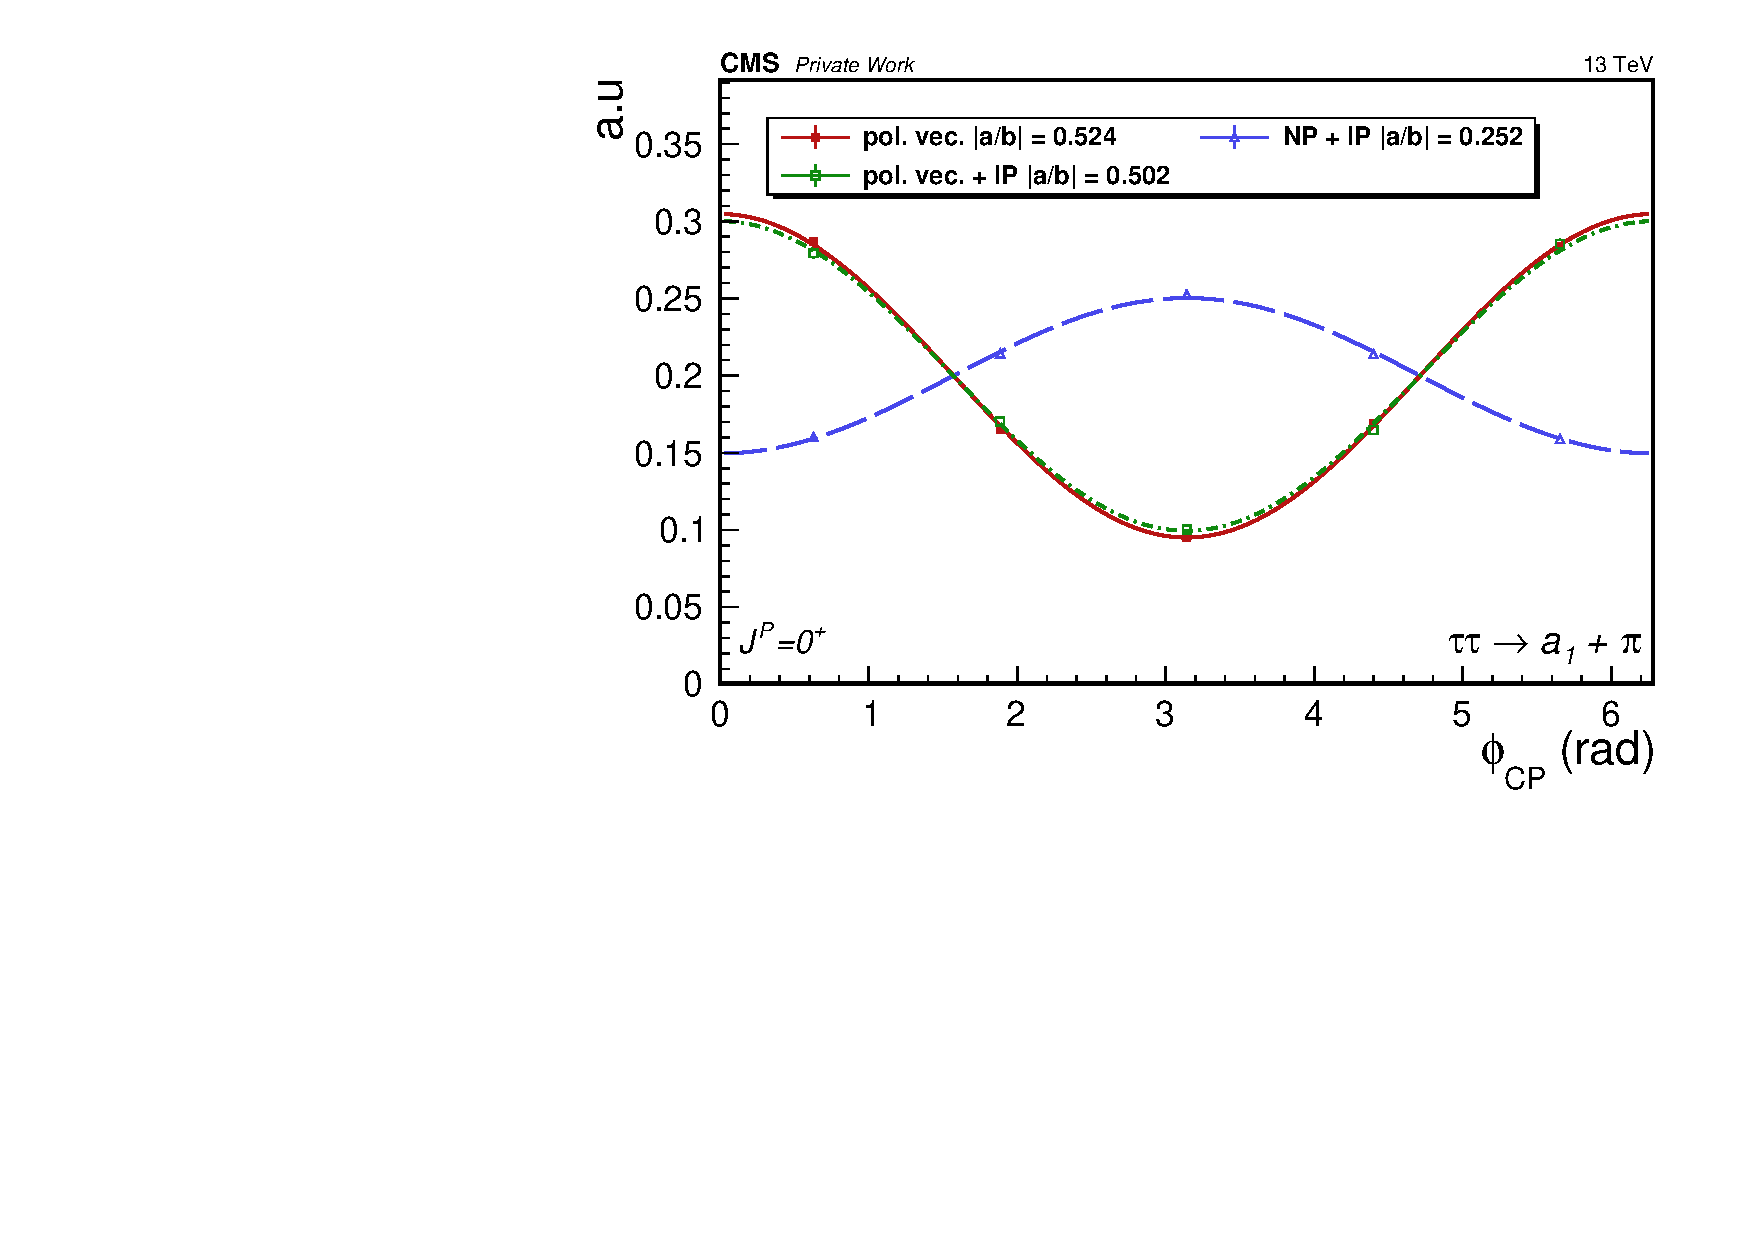
\includegraphics[width=\linewidth]{Chapitre6/Images/A1PION/A1PION_even_gen.pdf} 
    \caption*{} 
    \vspace{0.5ex}
  \end{subfigure}%% 
  \begin{subfigure}[b]{0.5\linewidth}
    \centering
    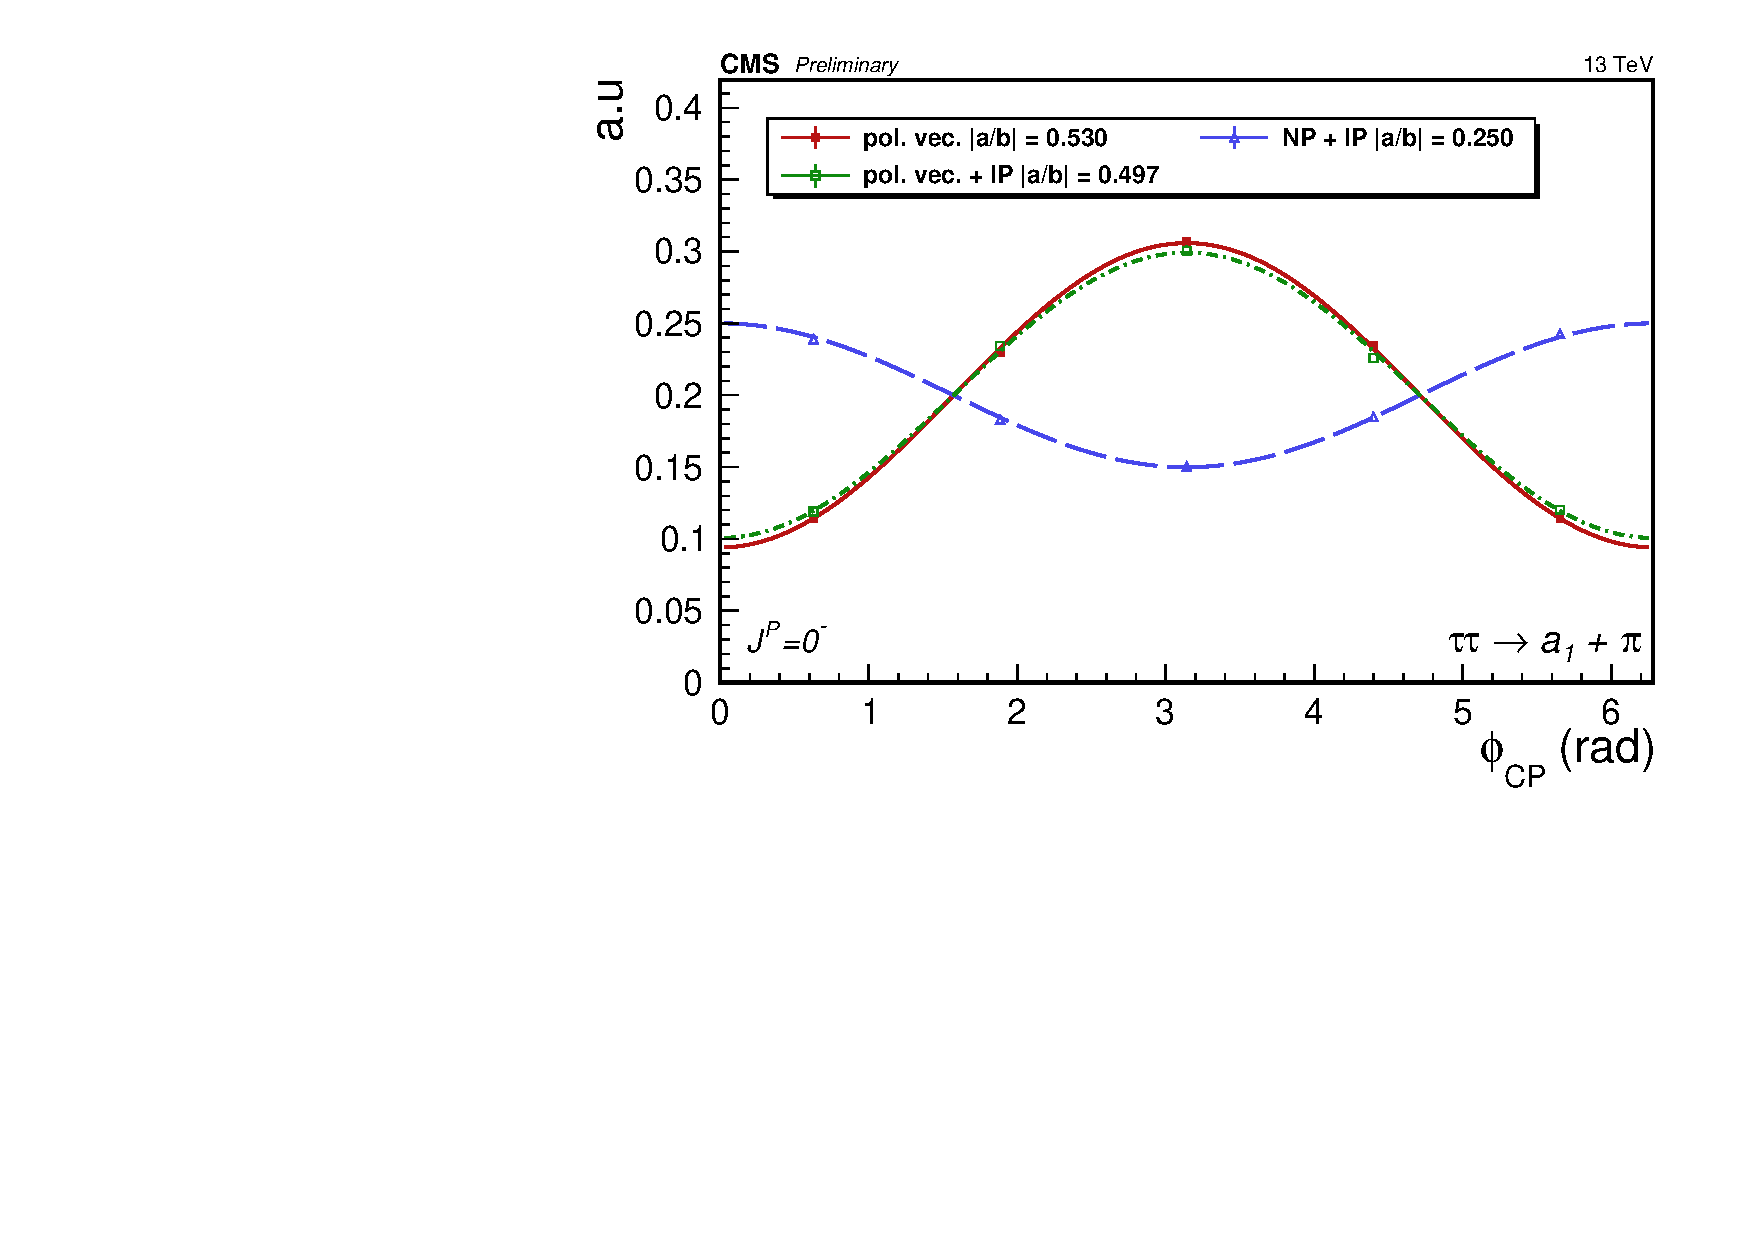
\includegraphics[width=\linewidth]{Chapitre6/Images/A1PION/A1PION_odd_gen.pdf} 
    \caption*{} 
    \vspace{0.5ex}
  \end{subfigure} 
  \caption{Distributions de $\phi_{CP}$ dans les canaux $\tau_h\tau_h\rightarrow X+\pi$, avec $X=\rho,a^{3pr}_1$, au niveau générateur pour l'état CP pair (gauche) et CP impair (droite) dans des évènements $ggH\to\tau\tau$.}
  \label{CPgenXPI}
\end{figure}


\begin{figure}[]
  \begin{subfigure}[b]{0.5\linewidth}
    \centering
    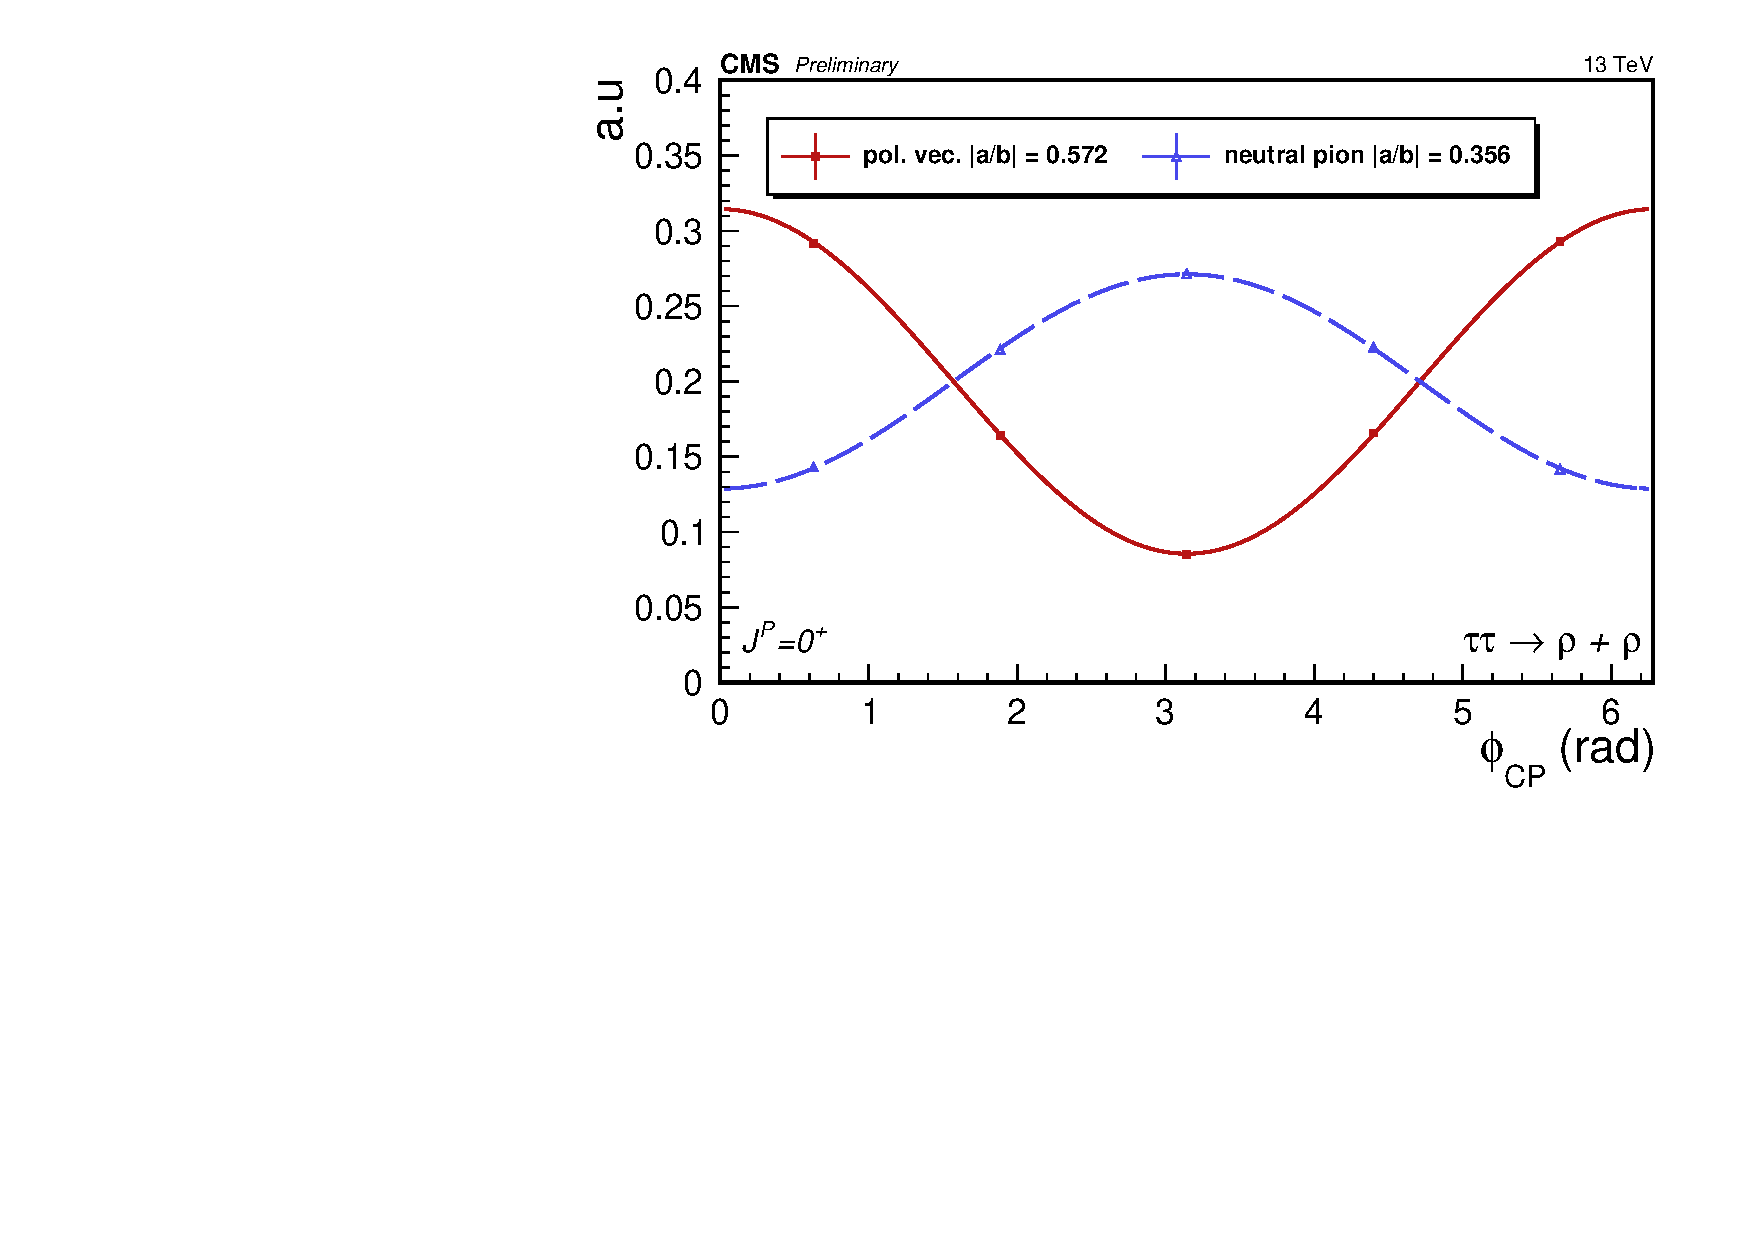
\includegraphics[width=\linewidth]{Chapitre6/Images/RHORHO/RHORHO_even_gen.pdf} 
    \caption*{} 
    \vspace{10mm}
  \end{subfigure}%% 
  \begin{subfigure}[b]{0.5\linewidth}
    \centering
    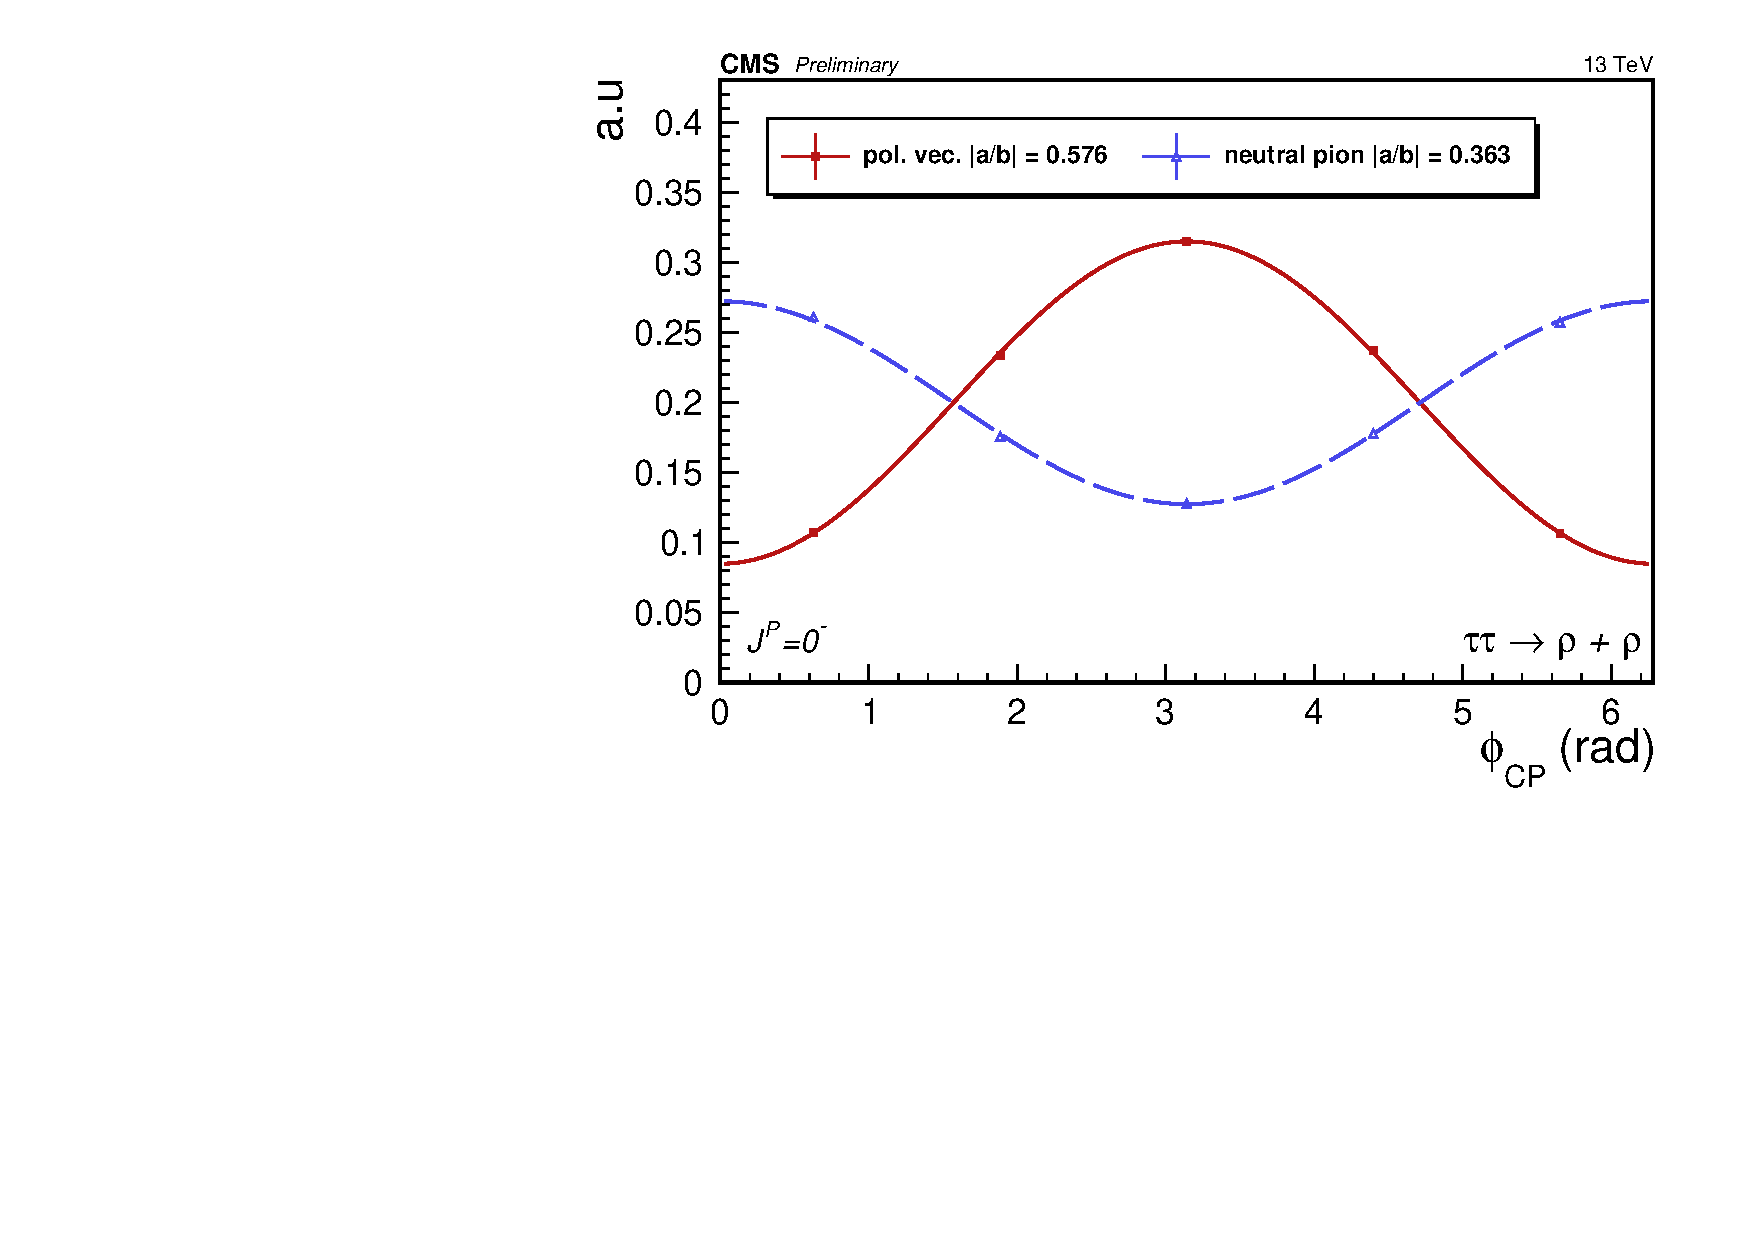
\includegraphics[width=\linewidth]{Chapitre6/Images/RHORHO/RHORHO_odd_gen.pdf} 
    \caption*{} 
    \vspace{10mm}
  \end{subfigure} 

  \begin{subfigure}[b]{0.5\linewidth}
    \centering
    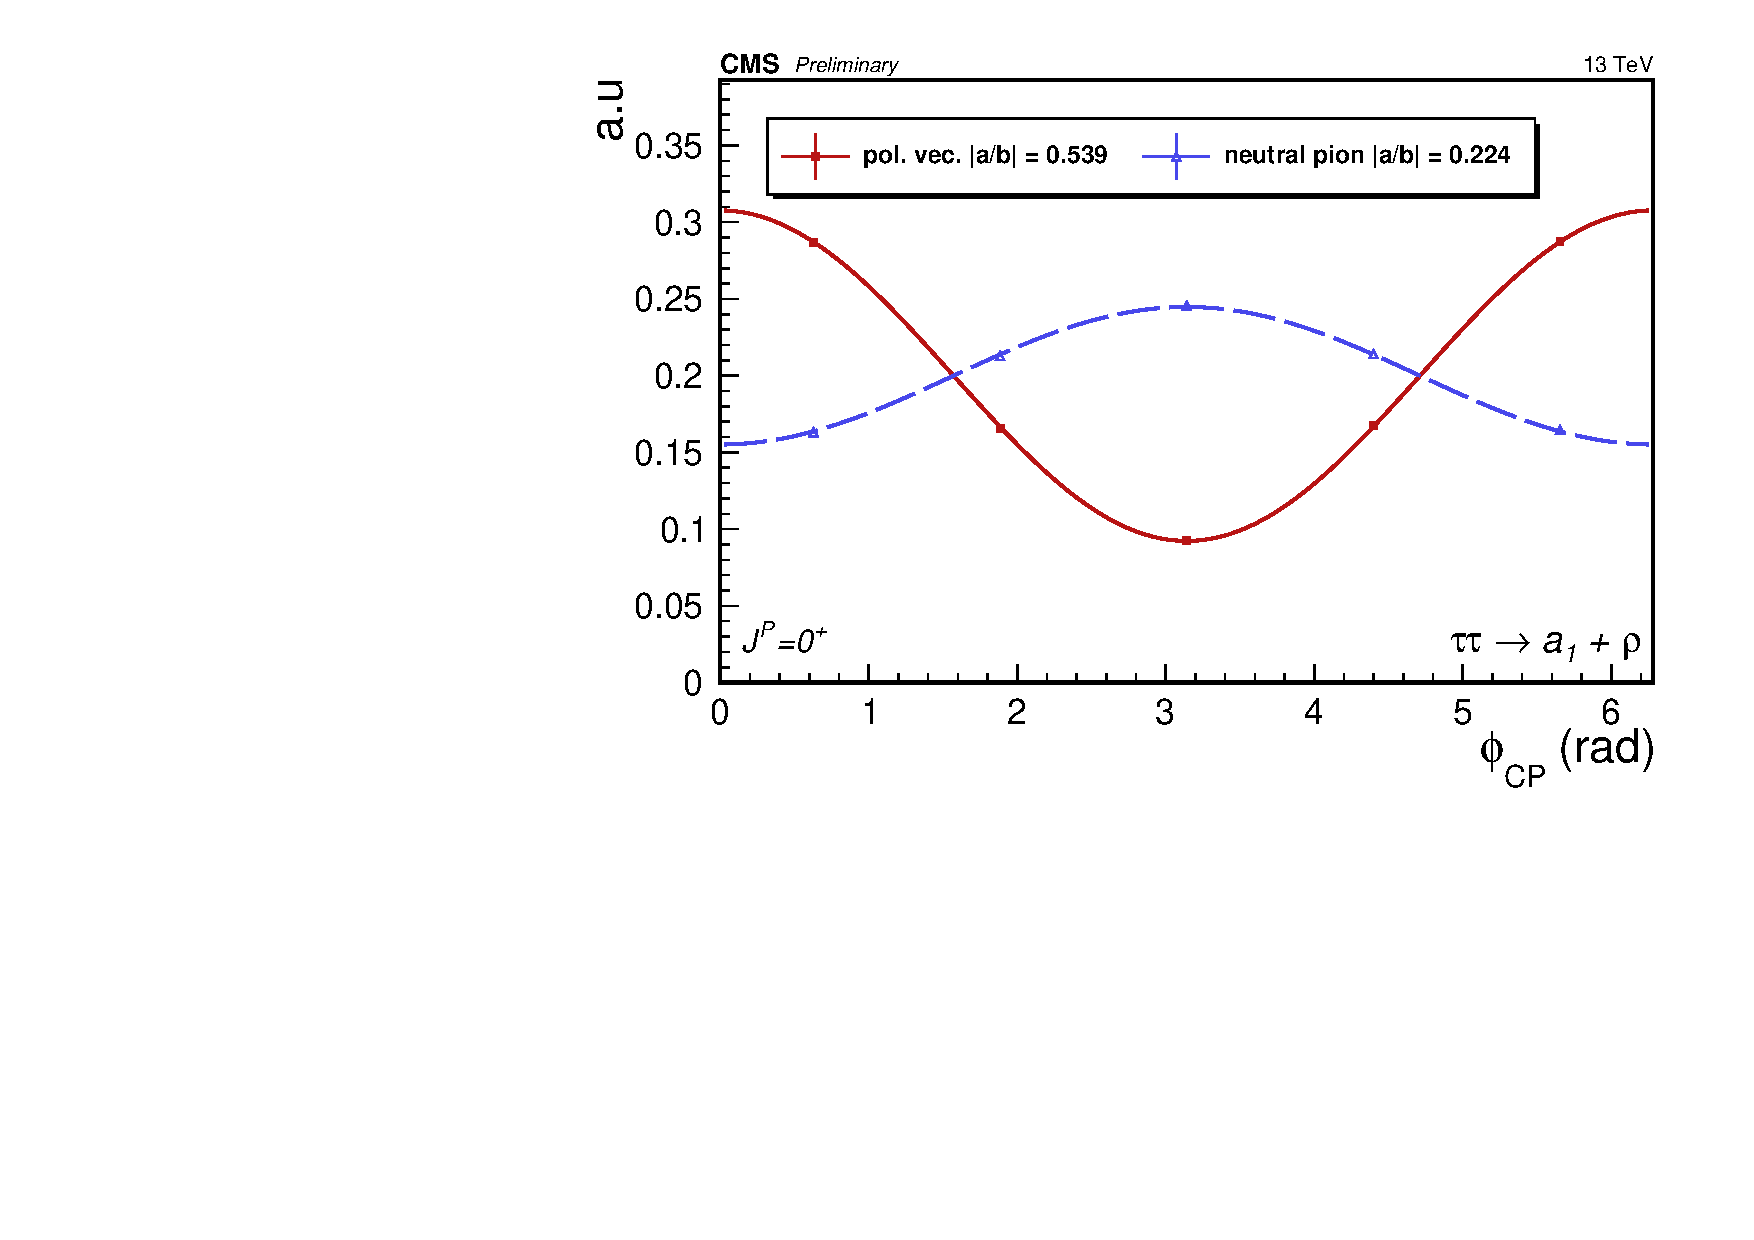
\includegraphics[width=\linewidth]{Chapitre6/Images/A1RHO/A1RHO_even_gen.pdf} 
    \caption*{} 
    \vspace{10mm}
  \end{subfigure}%% 
  \begin{subfigure}[b]{0.5\linewidth}
    \centering
    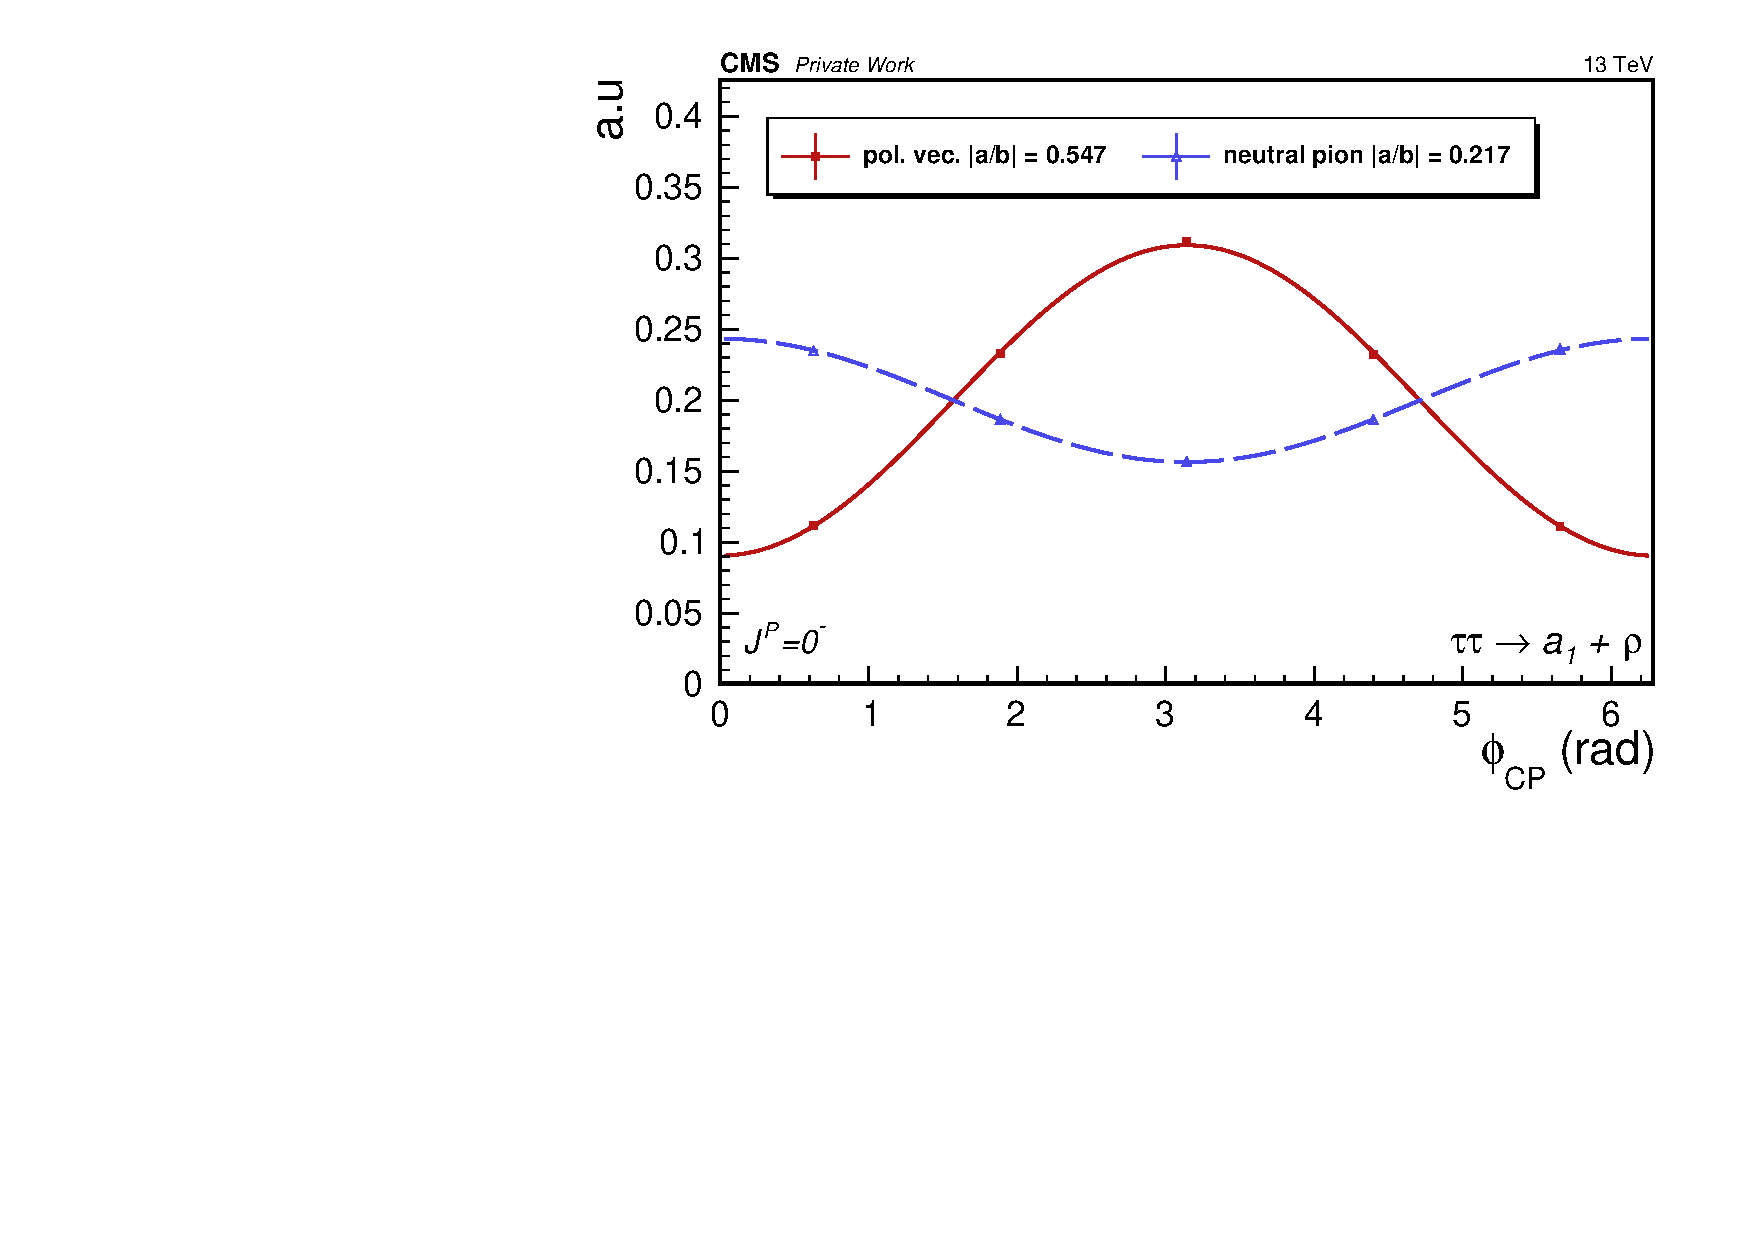
\includegraphics[width=\linewidth]{Chapitre6/Images/A1RHO/A1RHO_odd_gen.pdf} 
    \caption*{} 
    \vspace{10mm}
  \end{subfigure} 

    \begin{subfigure}[b]{0.5\linewidth}
    \centering
    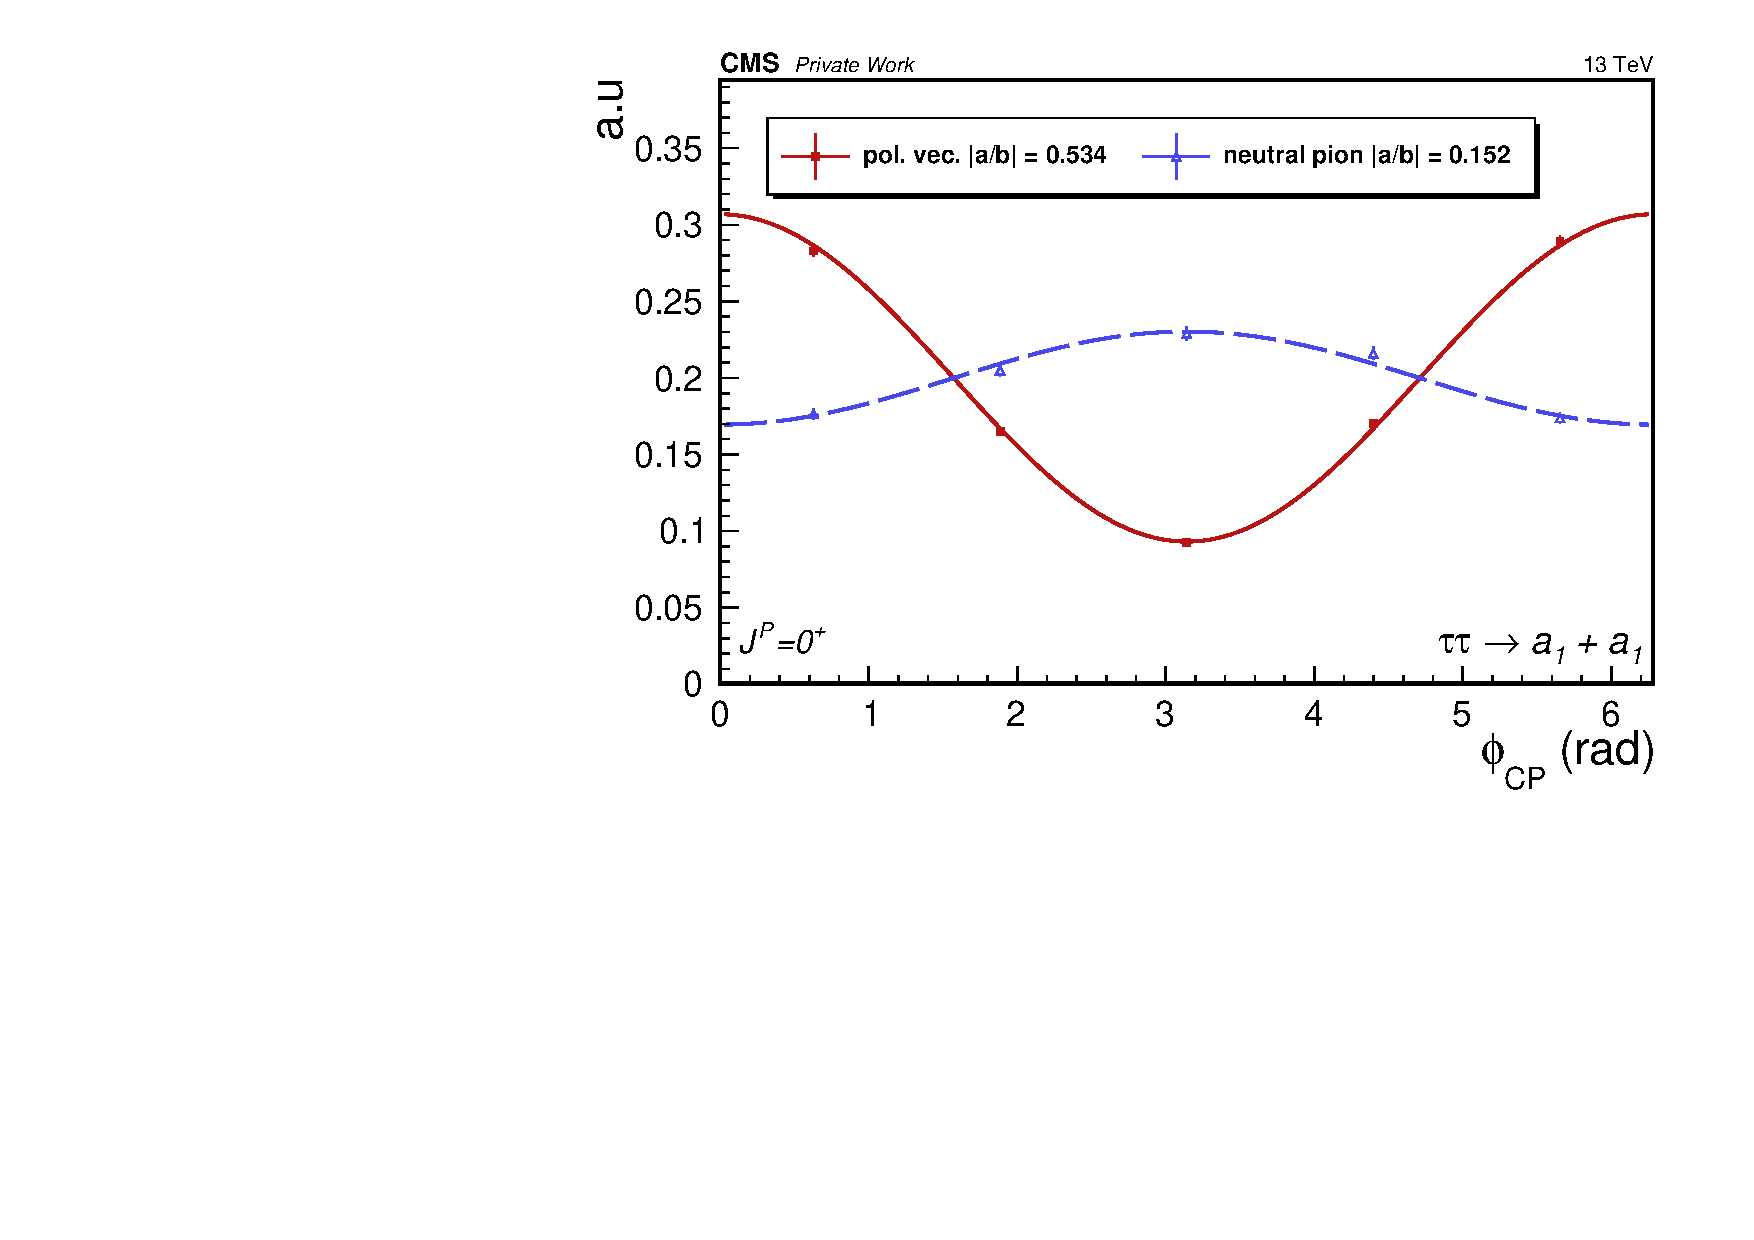
\includegraphics[width=\linewidth]{Chapitre6/Images/A1A1/A1A1_even_gen.pdf} 
    \caption*{} 
    \vspace{0.5ex}
  \end{subfigure}%% 
  \begin{subfigure}[b]{0.5\linewidth}
    \centering
    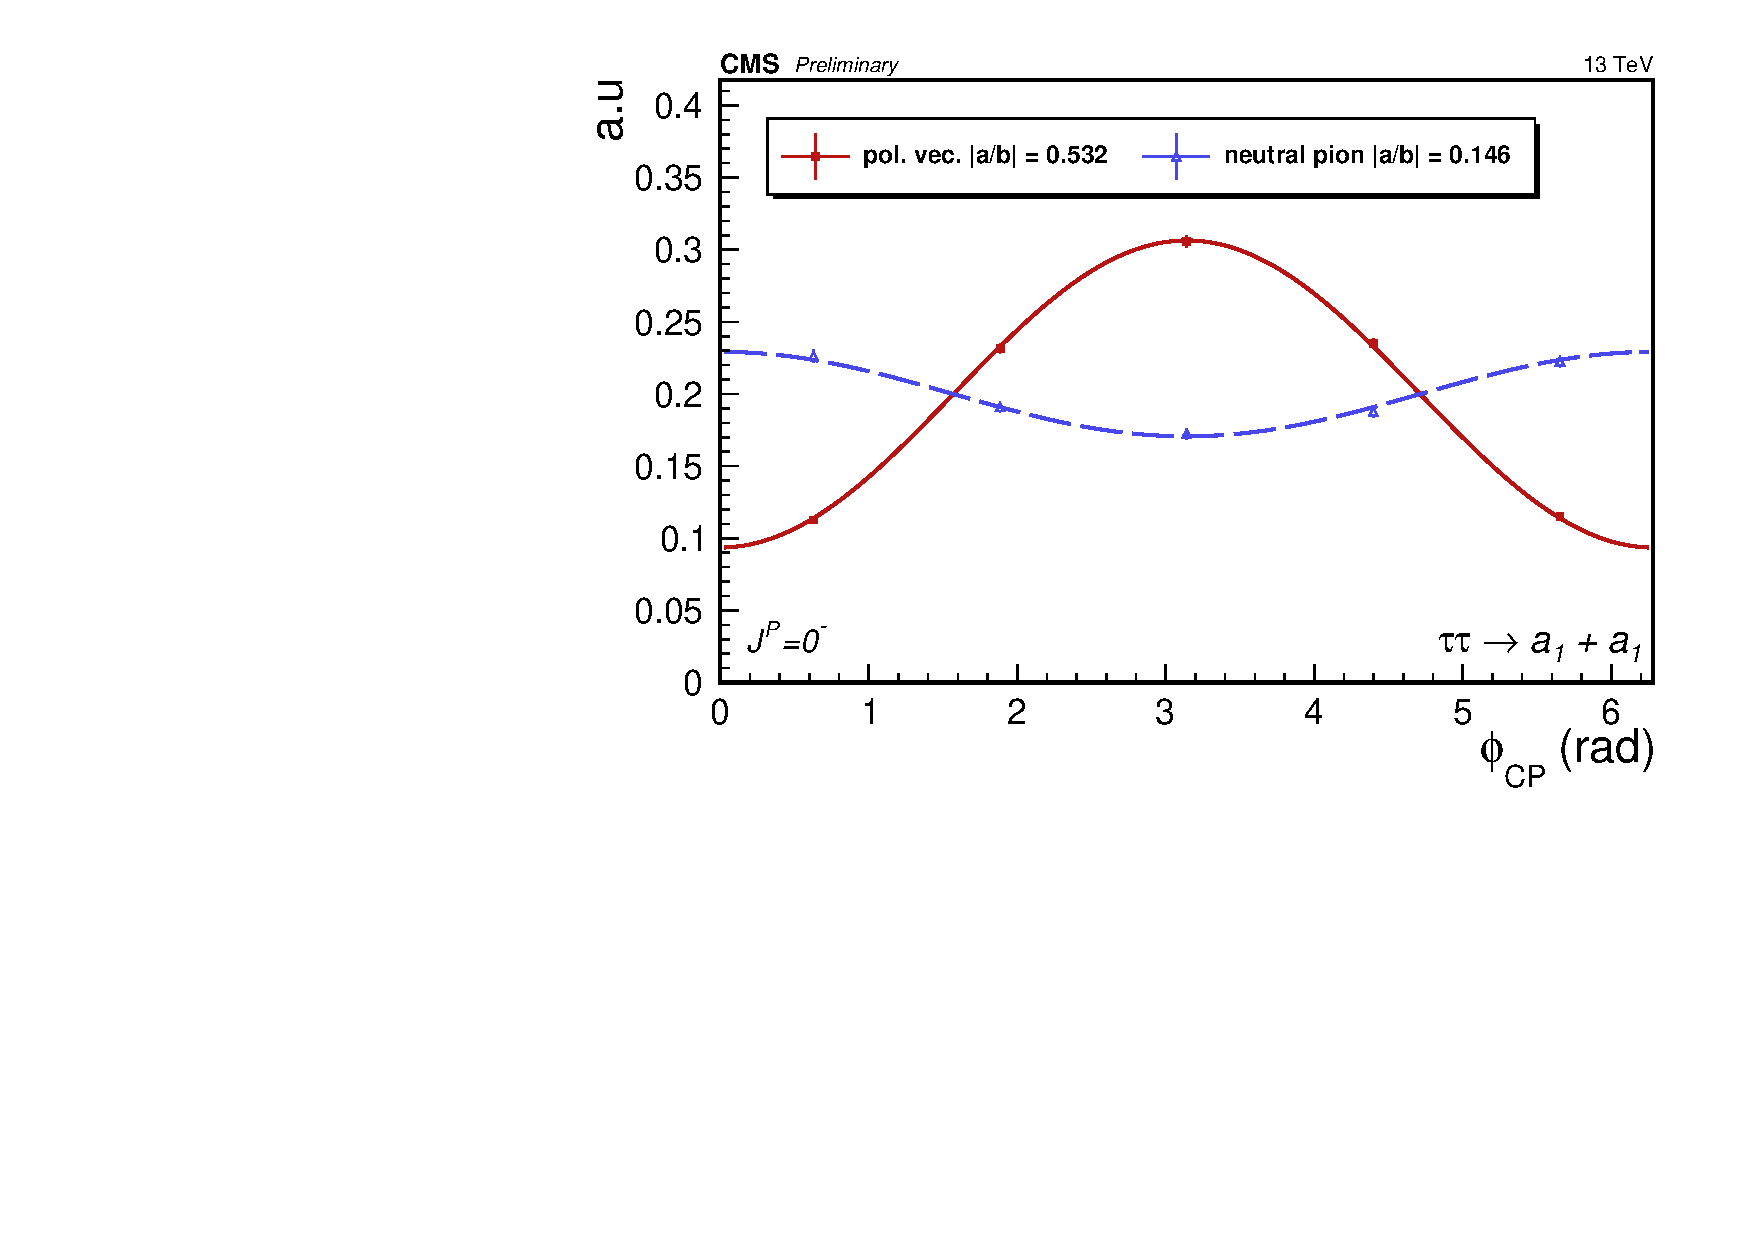
\includegraphics[width=\linewidth]{Chapitre6/Images/A1A1/A1A1_odd_gen.pdf} 
    \caption*{} 
    \vspace{0.5ex}
  \end{subfigure} 
  \caption{Distributions de $\phi_{CP}$ dans les canaux $\tau_h\tau_h\rightarrow X+\pi$, avec $X=\pi,\rho,a^{3pr}_1$, au niveau générateur pour l'état CP pair (gauche) et CP impair (droite) dans des évènements $ggH\to\tau\tau$.}
  \label{CPgen}
\end{figure}

\subsection{Performances au niveau générateur}

Le premier résultat de cette étude montre que les performances du vecteur polarimétrique et du paramètre d'impact sont égales dans le canal $\tau_h\tau_h\rightarrow\pi\pi$ (Fig. \ref{CPgenPIPI}). Ce mode de désintégration est le seul où le paramètre d'impact représente réellement le plan de désintégration du lepton tau. Ce dernier comporte alors autant d'information sur l'état CP que le vecteur polarimétrique qui est représenté par le vecteur suivant la direction de l'impulsion du pion mais de sens opposé. Cela justifie également qu'aucun gain de sensibilité significatif n'est observé dans les canaux $\tau_h\tau_h\rightarrow\rho,a_1^{3pr}+\pi$ lorsque le vecteur polarimétrique est appliqué sur le pion plutôt que le paramètre d'impact (Fig. \ref{CPgenXPI}) et montre que le gain global obtenu est majoritairement lié au remplacement de la méthode du pion neutre. D'autre part, le plus grand potentiel d'optimisation se trouve dans les canaux intégrant une résonance $a_1^{3pr}$ puisque contrairement au vecteur polarimétrique, la méthode du pion neutre ne tient pas compte de la totalité des produits de désintégration visibles du lepton tau (Fig. \ref{CPgen}). Ces résultats au niveau générateur permettent de fixer quelques limites sur les prospectives de déploiement du vecteur polarimétrique au niveau reconstruit.  \\ 


%%%%%%%%%%%%%%%%%%%%
%%%%%%%%%%%%%%%%%%%%

%%%%%%%%%%%%%%%%%%%%
%%%%%%%%%%%%%%%%%%%%

\subsection{Performances au niveau reconstruit}

\begin{figure}[!ht]
    \centering
    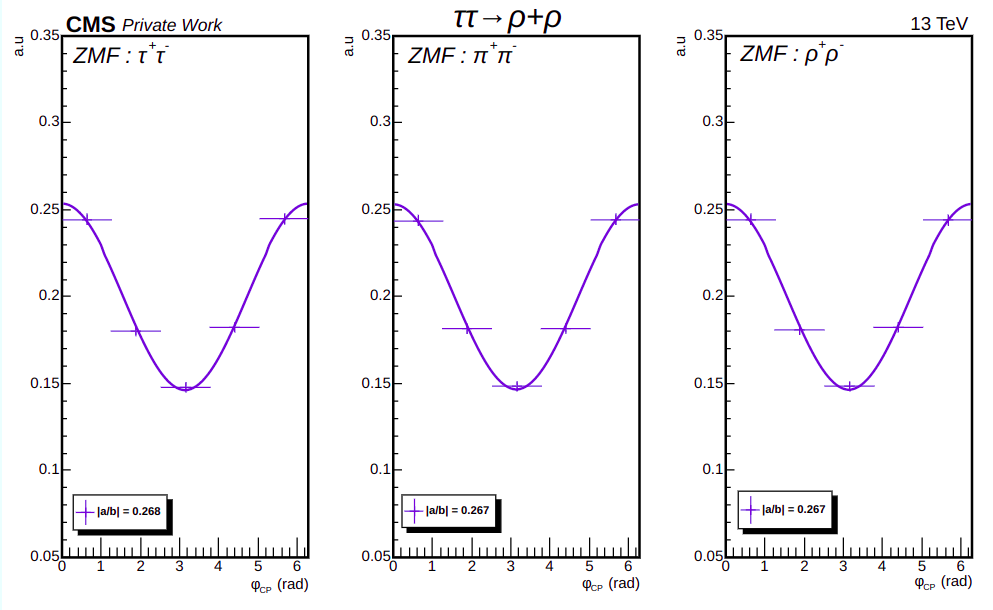
\includegraphics[scale=0.37]{Chapitre6/Images/ZMFreco.png} 
  \caption{Distribution de $\phi_{CP}$ dans le canal $\tau_h\tau_h\rightarrow\rho\rho$ au niveau reconstruit dans le référentiel au repos du boson de Higgs (gauche), des pions chargés (centre) et des mésons rho (droite).}
  \label{ZMFreco}
\end{figure}

La même étude est ensuite portée au niveau reconstruit. L'utilisation des algorithmes SVFit et FastMTT ne permettent pas d'obtenir une distribution de $\phi_{CP}$ physique lorsqu'ils sont employés pour la reconstruction de la paire de leptons tau et l'application de la méthode du vecteur polarimétrique. La figure \ref{TauRes} de la section \ref{taualgo} montre que l'algorithme SVFit est plus performant dans la reconstruction de l'énergie et de l'impulsion tandis que FastMTT offre une meilleure résolution angulaire. Dans la suite, les quadrivecteurs des leptons tau utilisés dans l'application de la méthode du vecteur polarimétrique sont construits à partir des quadrivecteurs issus des deux algorithmes tels que :  

\begin{equation}
    p_{\tau} = (E^{\text{\tiny SVFit}}_{\tau},\vec{n}_{\tau}^{\text{\tiny FastMTT}}\times P^{\text{\tiny SVFit}}_{\tau}).
\end{equation}

\begin{figure}[!ht]
  \begin{subfigure}[b]{0.5\linewidth}
    \centering
    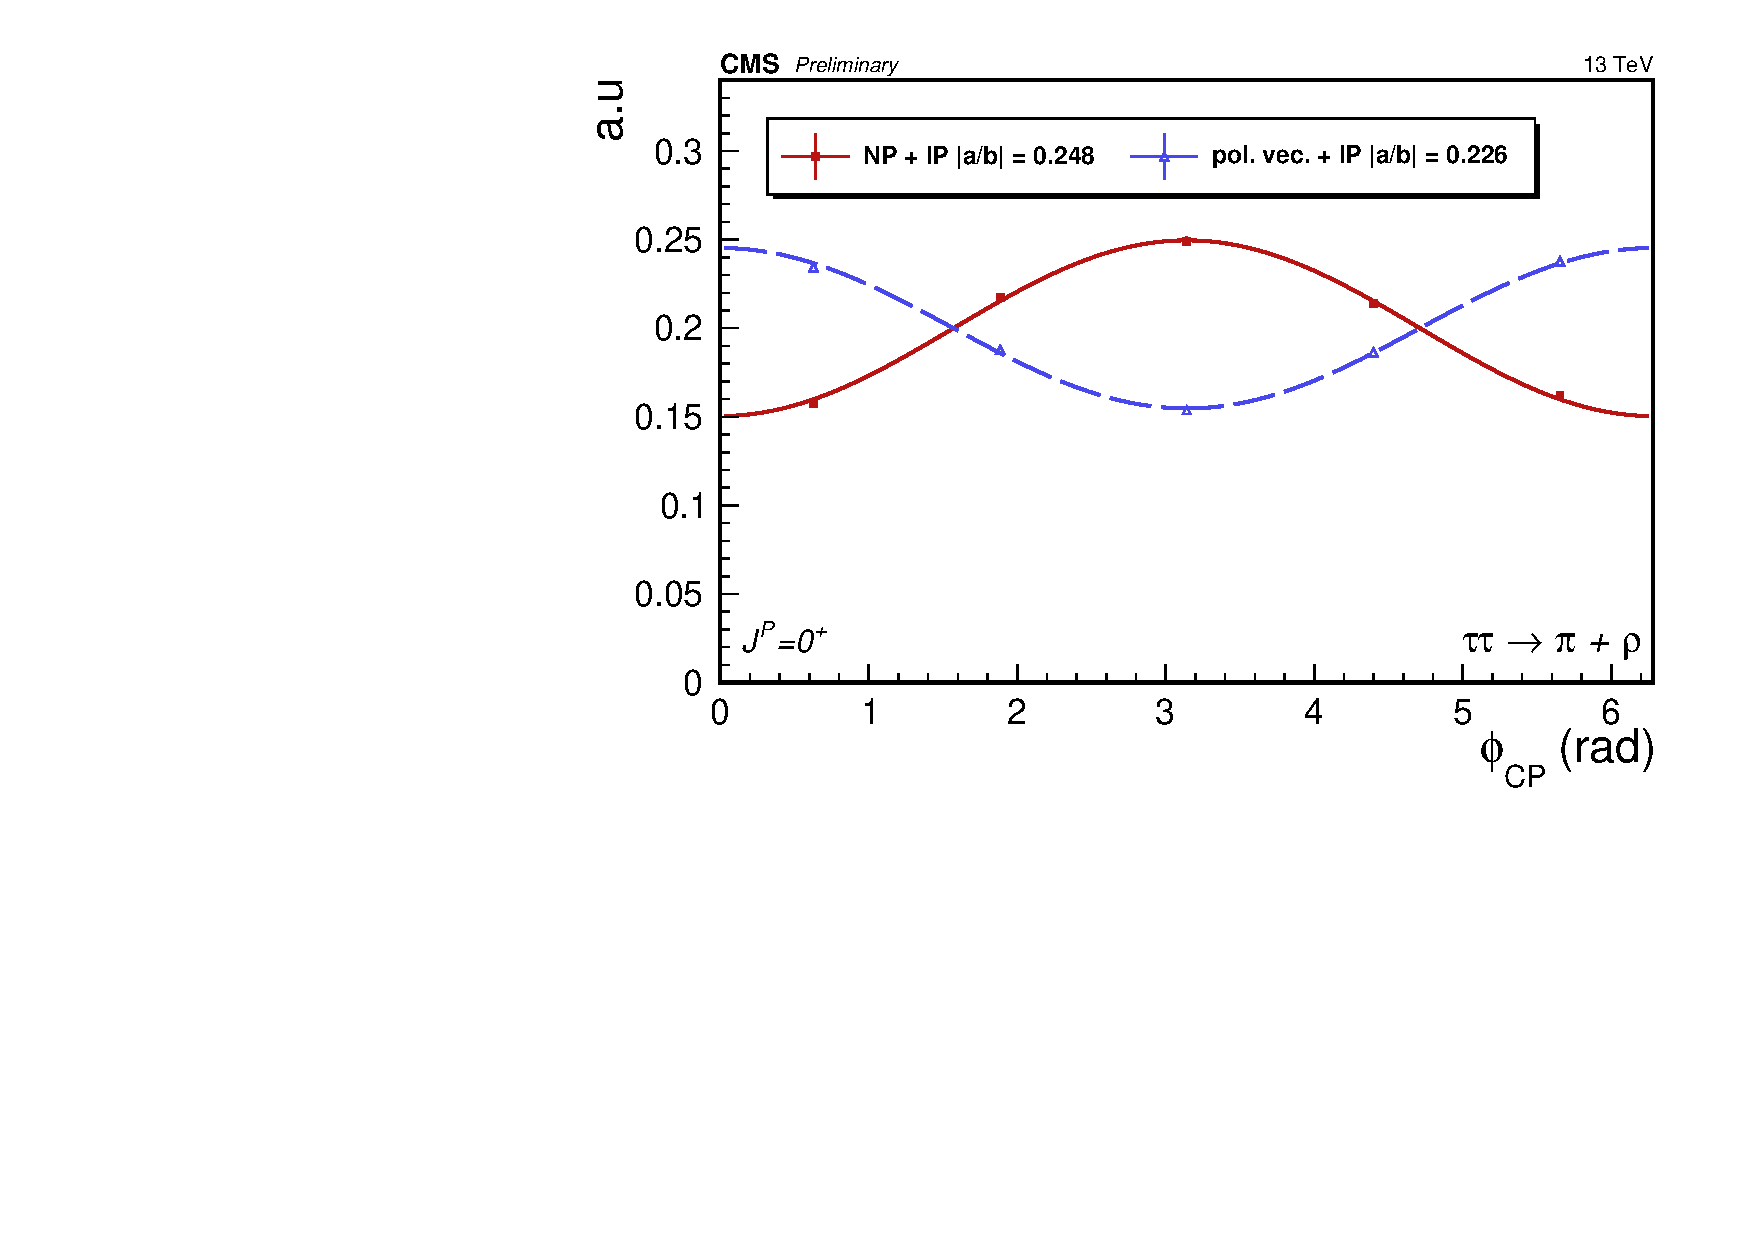
\includegraphics[width=\linewidth]{Chapitre6/Images/RHOPION/RHOPION_even_reco.pdf} 
    \caption*{} 
    \vspace{0.5ex}
  \end{subfigure}%% 
  \begin{subfigure}[b]{0.5\linewidth}
    \centering
    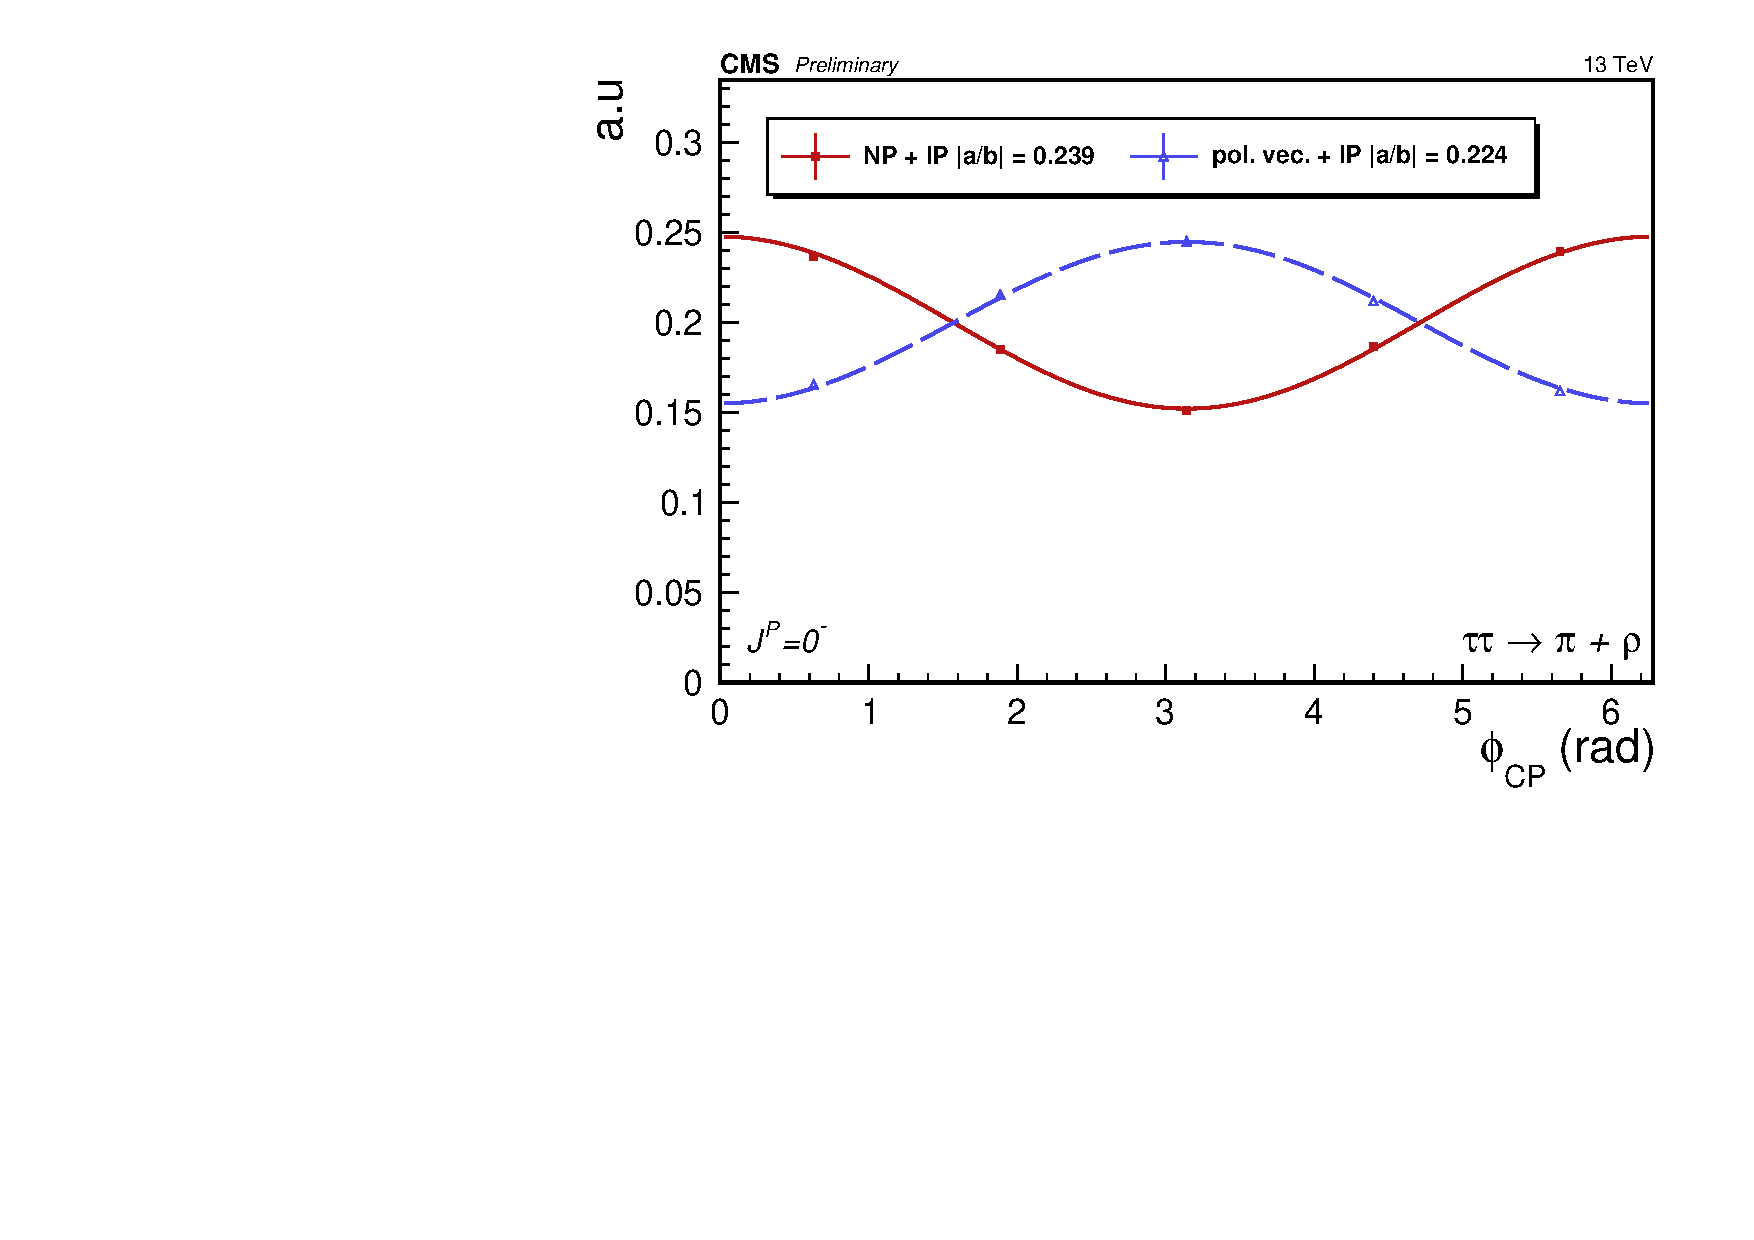
\includegraphics[width=\linewidth]{Chapitre6/Images/RHOPION/RHOPION_odd_reco.pdf} 
    \caption*{} 
    \vspace{0.5ex}
  \end{subfigure} 

  \begin{subfigure}[b]{0.5\linewidth}
    \centering
    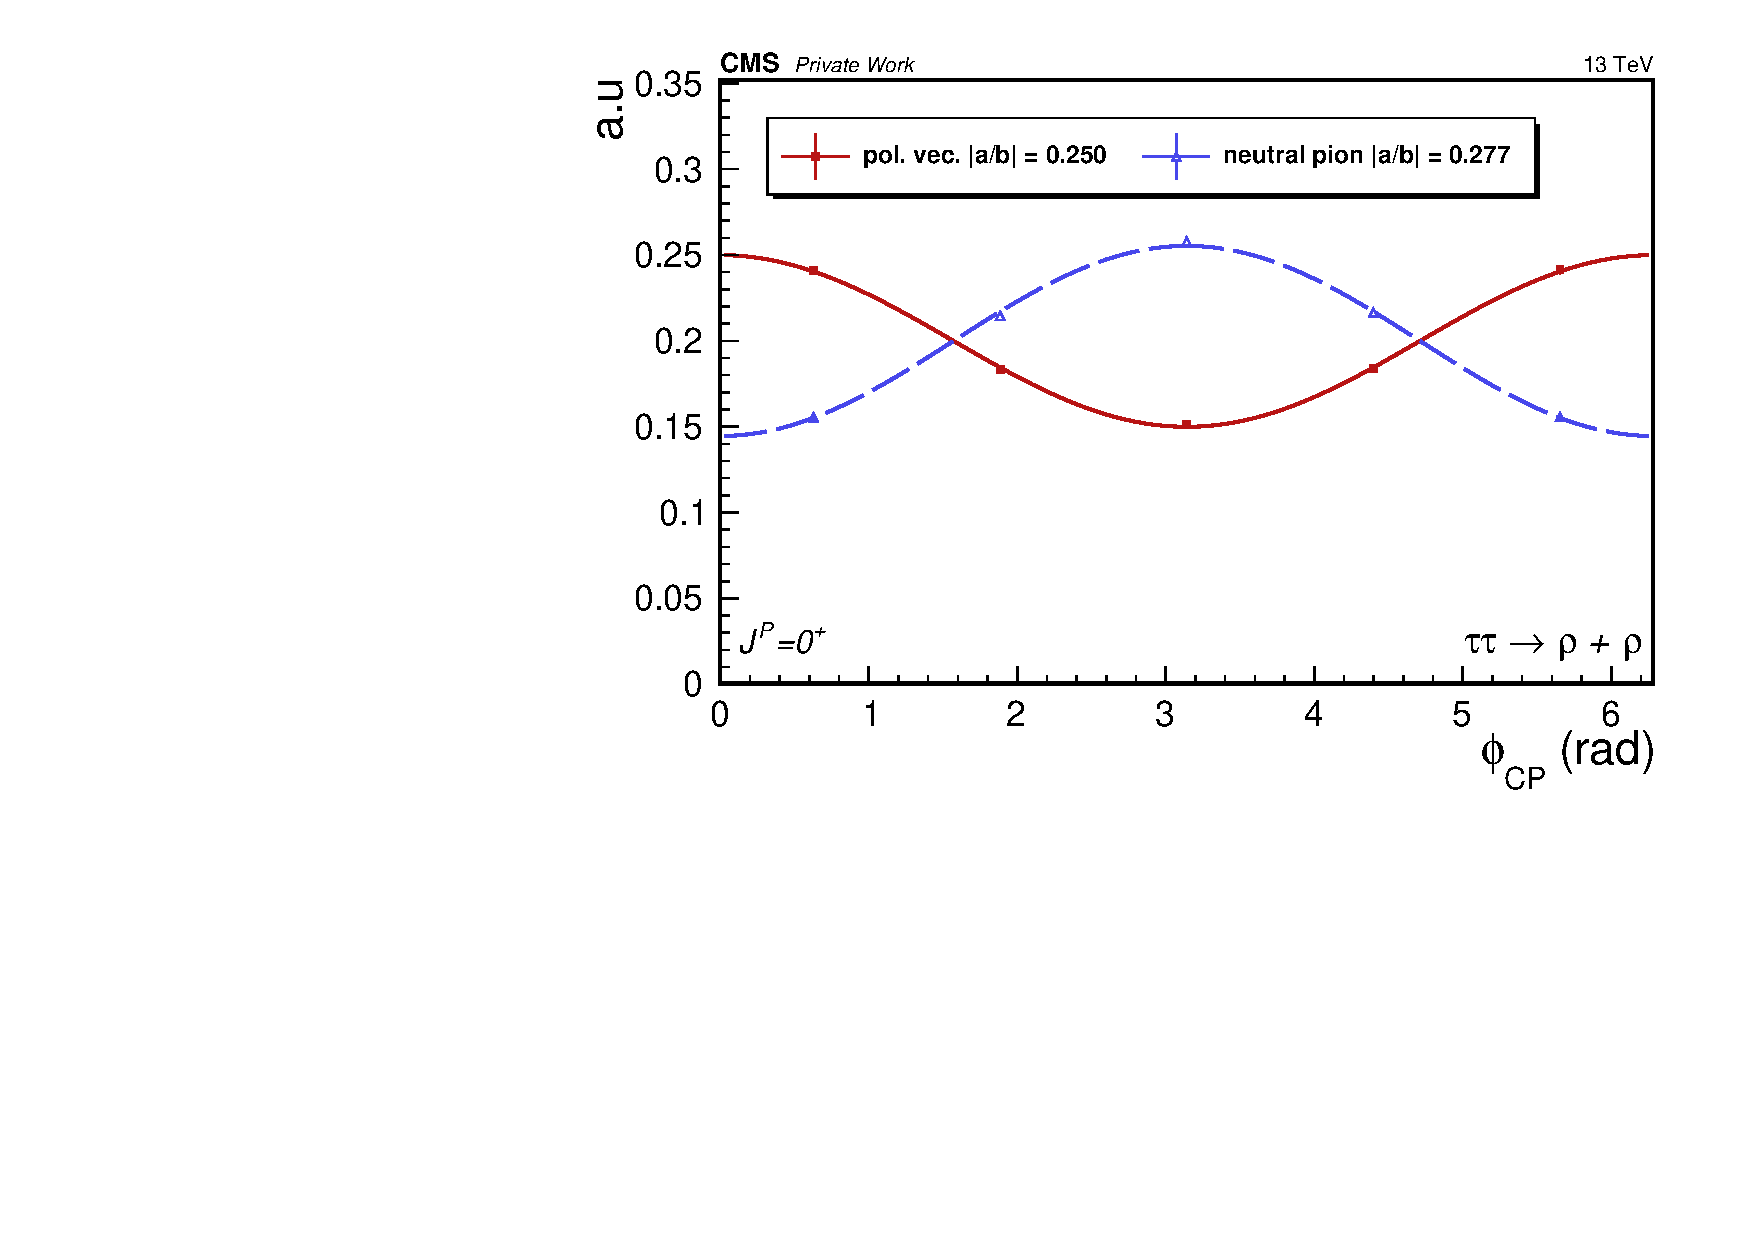
\includegraphics[width=\linewidth]{Chapitre6/Images/RHORHO/RHORHO_even_reco.pdf} 
    \caption*{} 
    \vspace{0.5ex}
  \end{subfigure}%% 
  \begin{subfigure}[b]{0.5\linewidth}
    \centering
    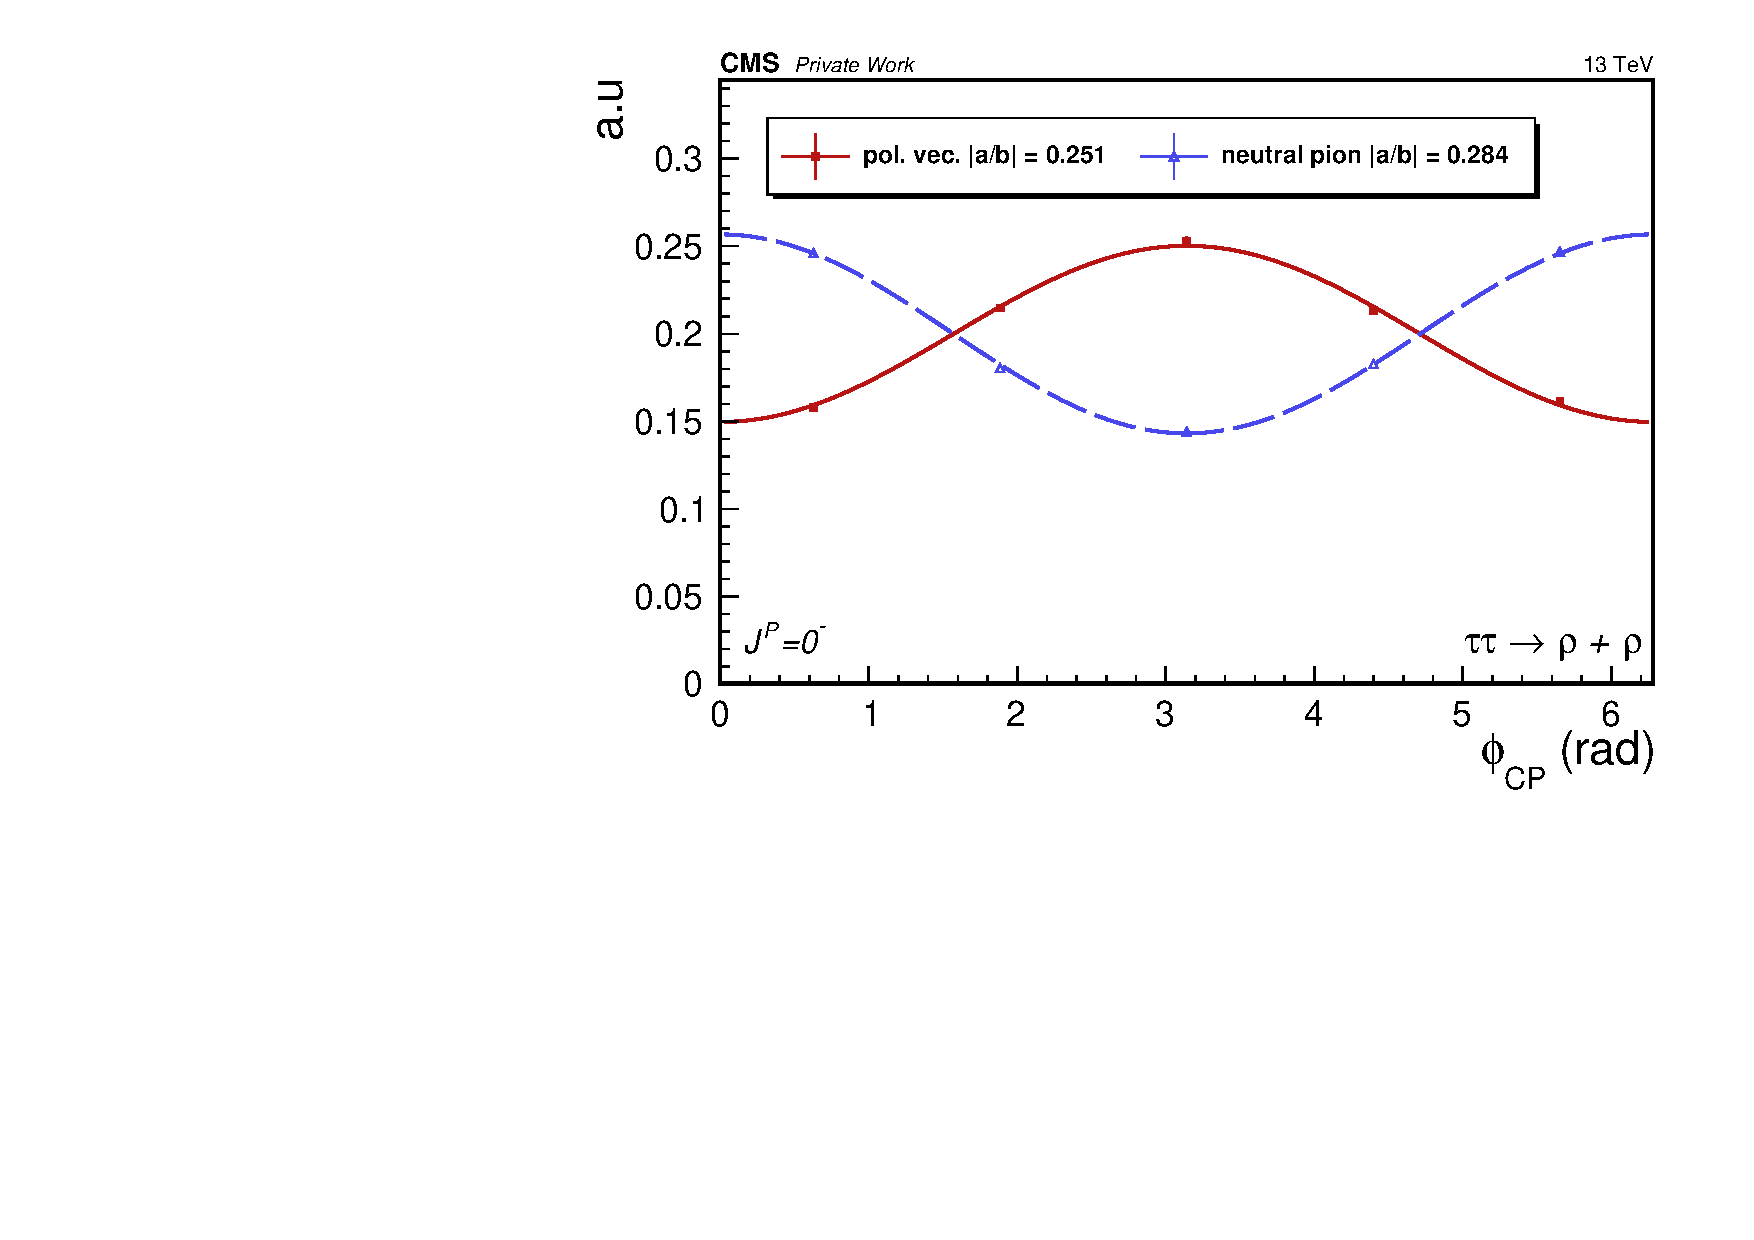
\includegraphics[width=\linewidth]{Chapitre6/Images/RHORHO/RHORHO_odd_reco.pdf} 
    \caption*{} 
    \vspace{0.5ex}
  \end{subfigure} 
  \caption{Distributions de $\phi_{CP}$ dans les canaux $\tau_h\tau_h\rightarrow X+\rho$, avec $X=\pi,\rho$, au niveau reconstruit pour l'état CP pair (gauche) et CP impair (droite) dans des évènements $ggH\to\tau\tau$.}
  \label{CPrecoXPI}
\end{figure}

\begin{figure}[]
    \begin{subfigure}[b]{0.5\linewidth}
    \centering
    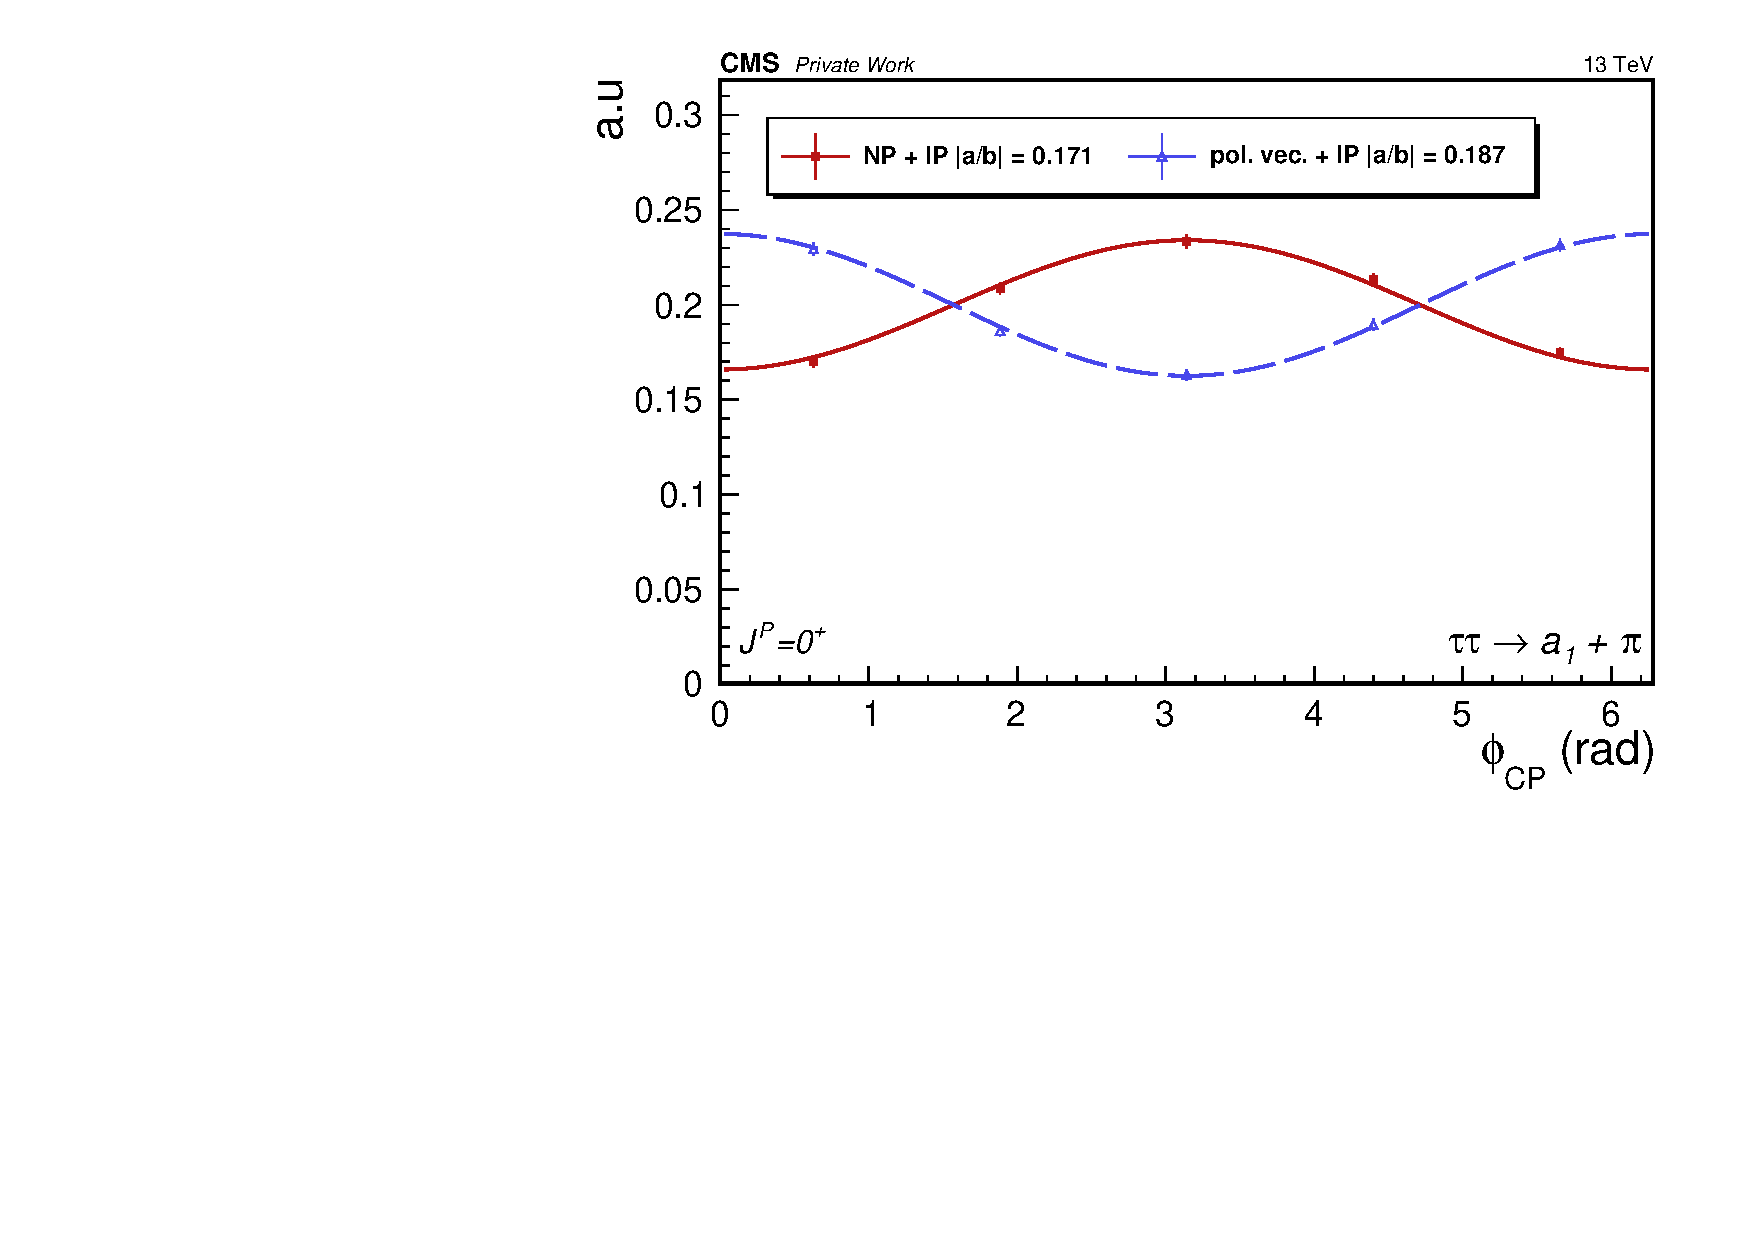
\includegraphics[width=\linewidth]{Chapitre6/Images/A1PION/A1PION_even_reco.pdf} 
    \caption*{} 
    \vspace{10mm}
  \end{subfigure}%% 
  \begin{subfigure}[b]{0.5\linewidth}
    \centering
    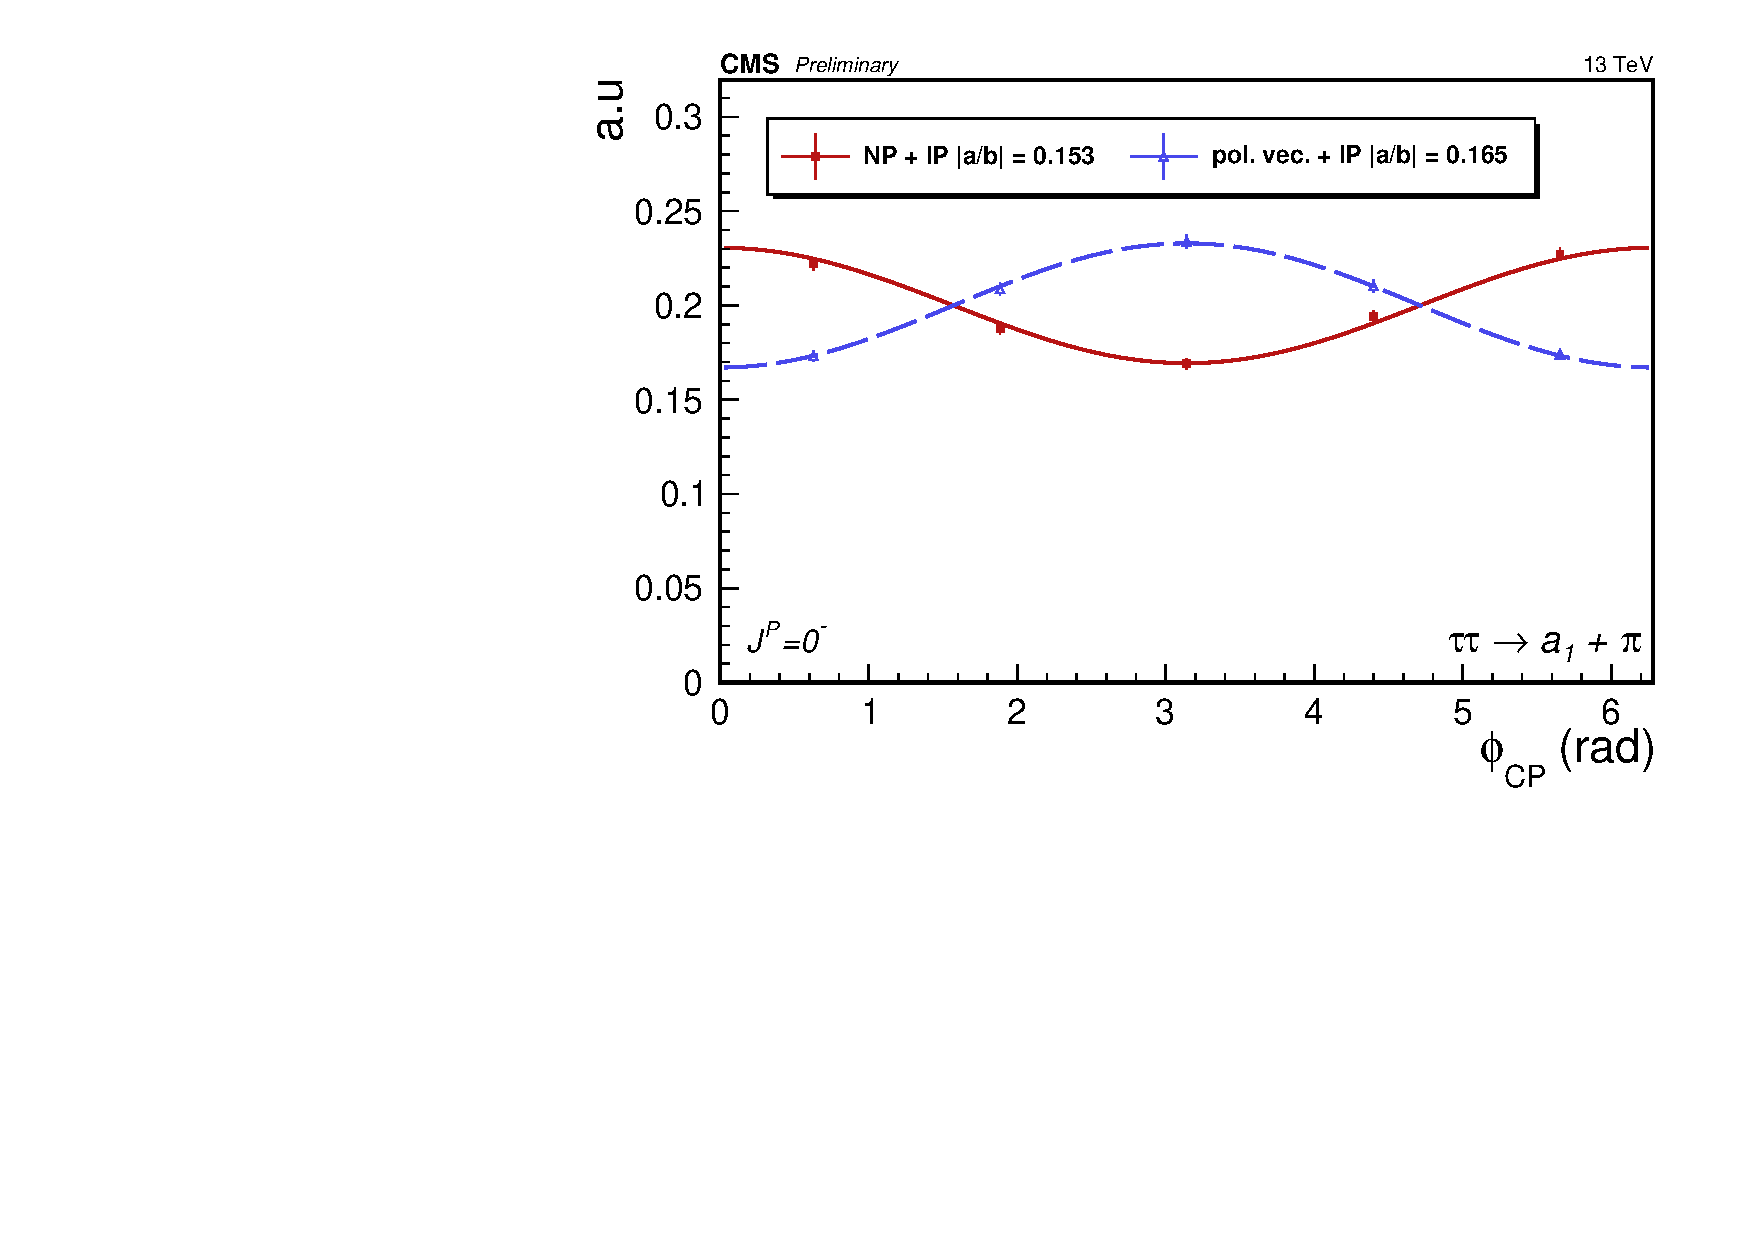
\includegraphics[width=\linewidth]{Chapitre6/Images/A1PION/A1PION_odd_reco.pdf} 
    \caption*{} 
    \vspace{10mm}
  \end{subfigure}

    \begin{subfigure}[b]{0.5\linewidth}
    \centering
    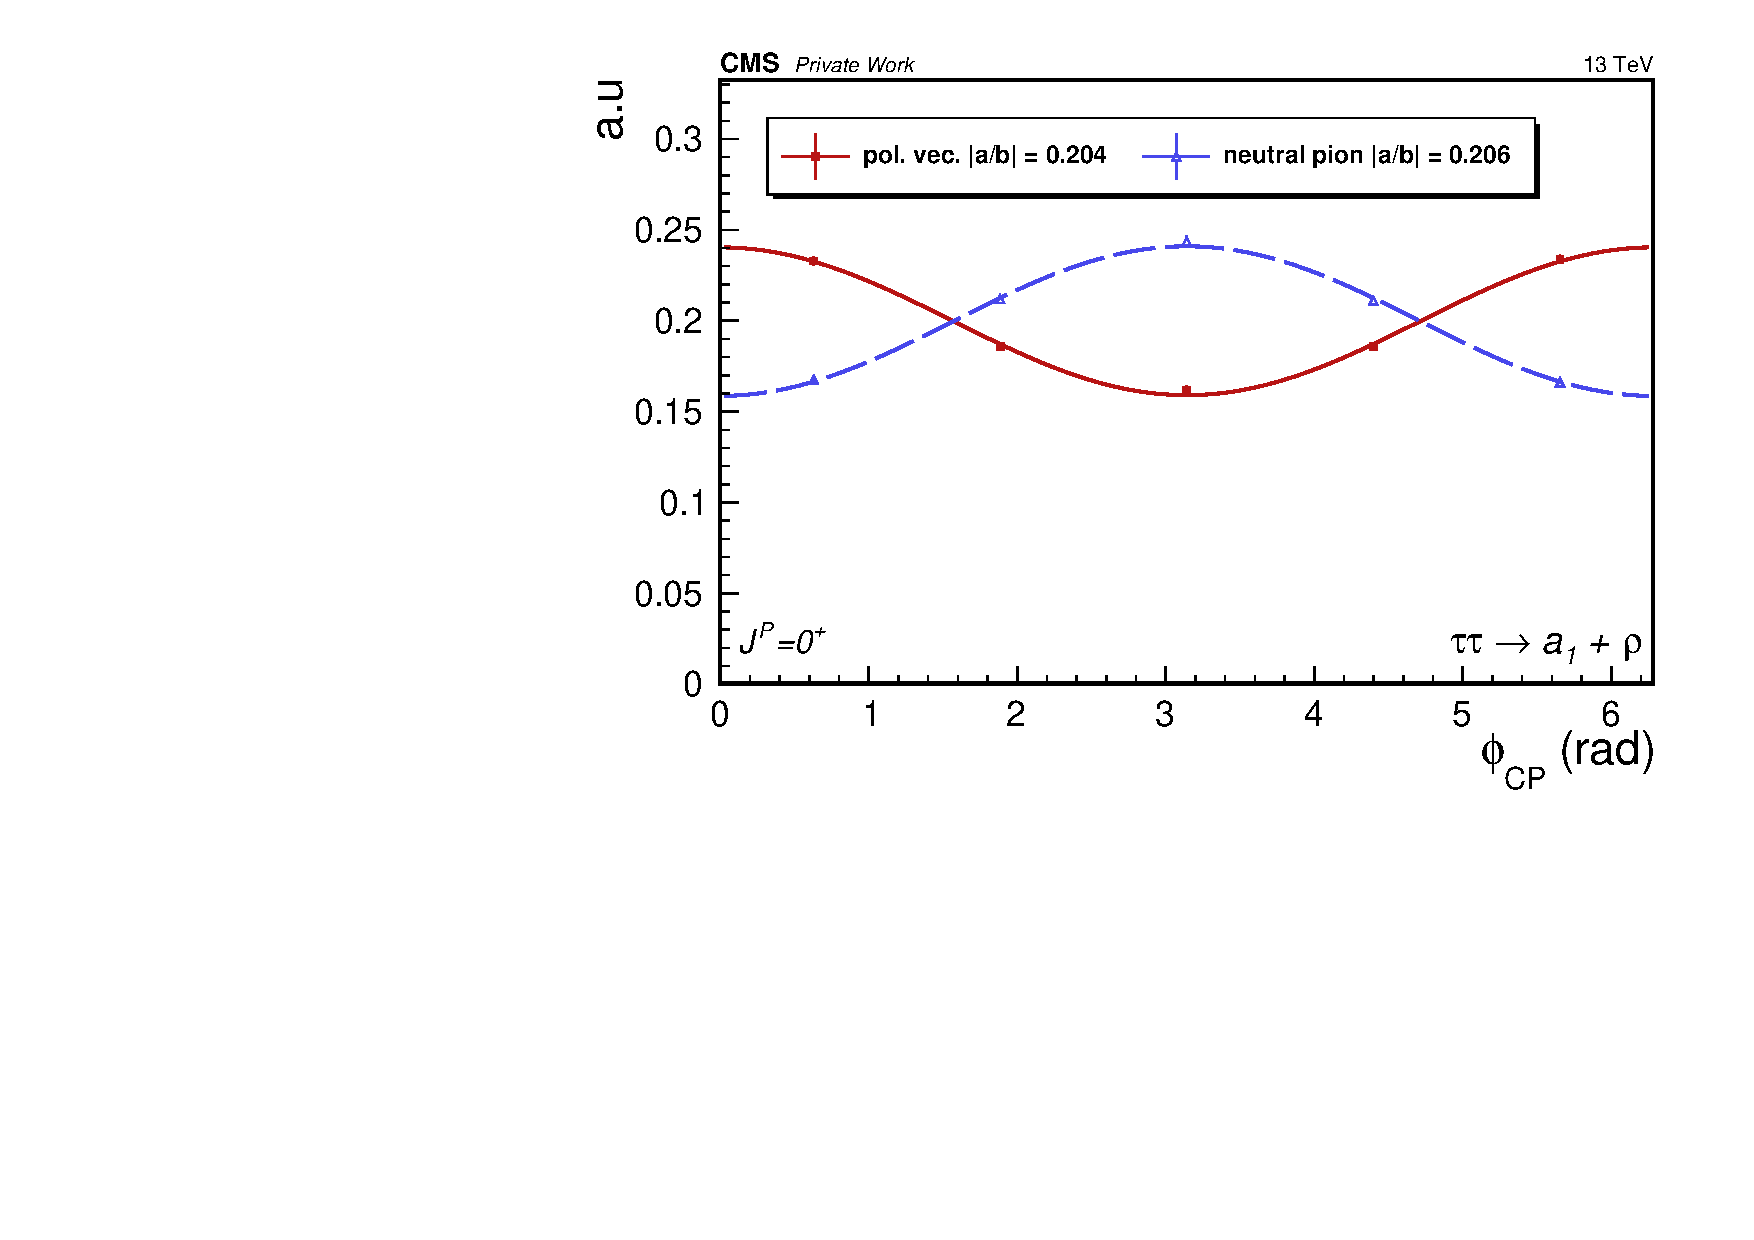
\includegraphics[width=\linewidth]{Chapitre6/Images/A1RHO/A1RHO_even_reco.pdf} 
    \caption*{} 
    \vspace{10mm}
  \end{subfigure}%% 
  \begin{subfigure}[b]{0.5\linewidth}
    \centering
    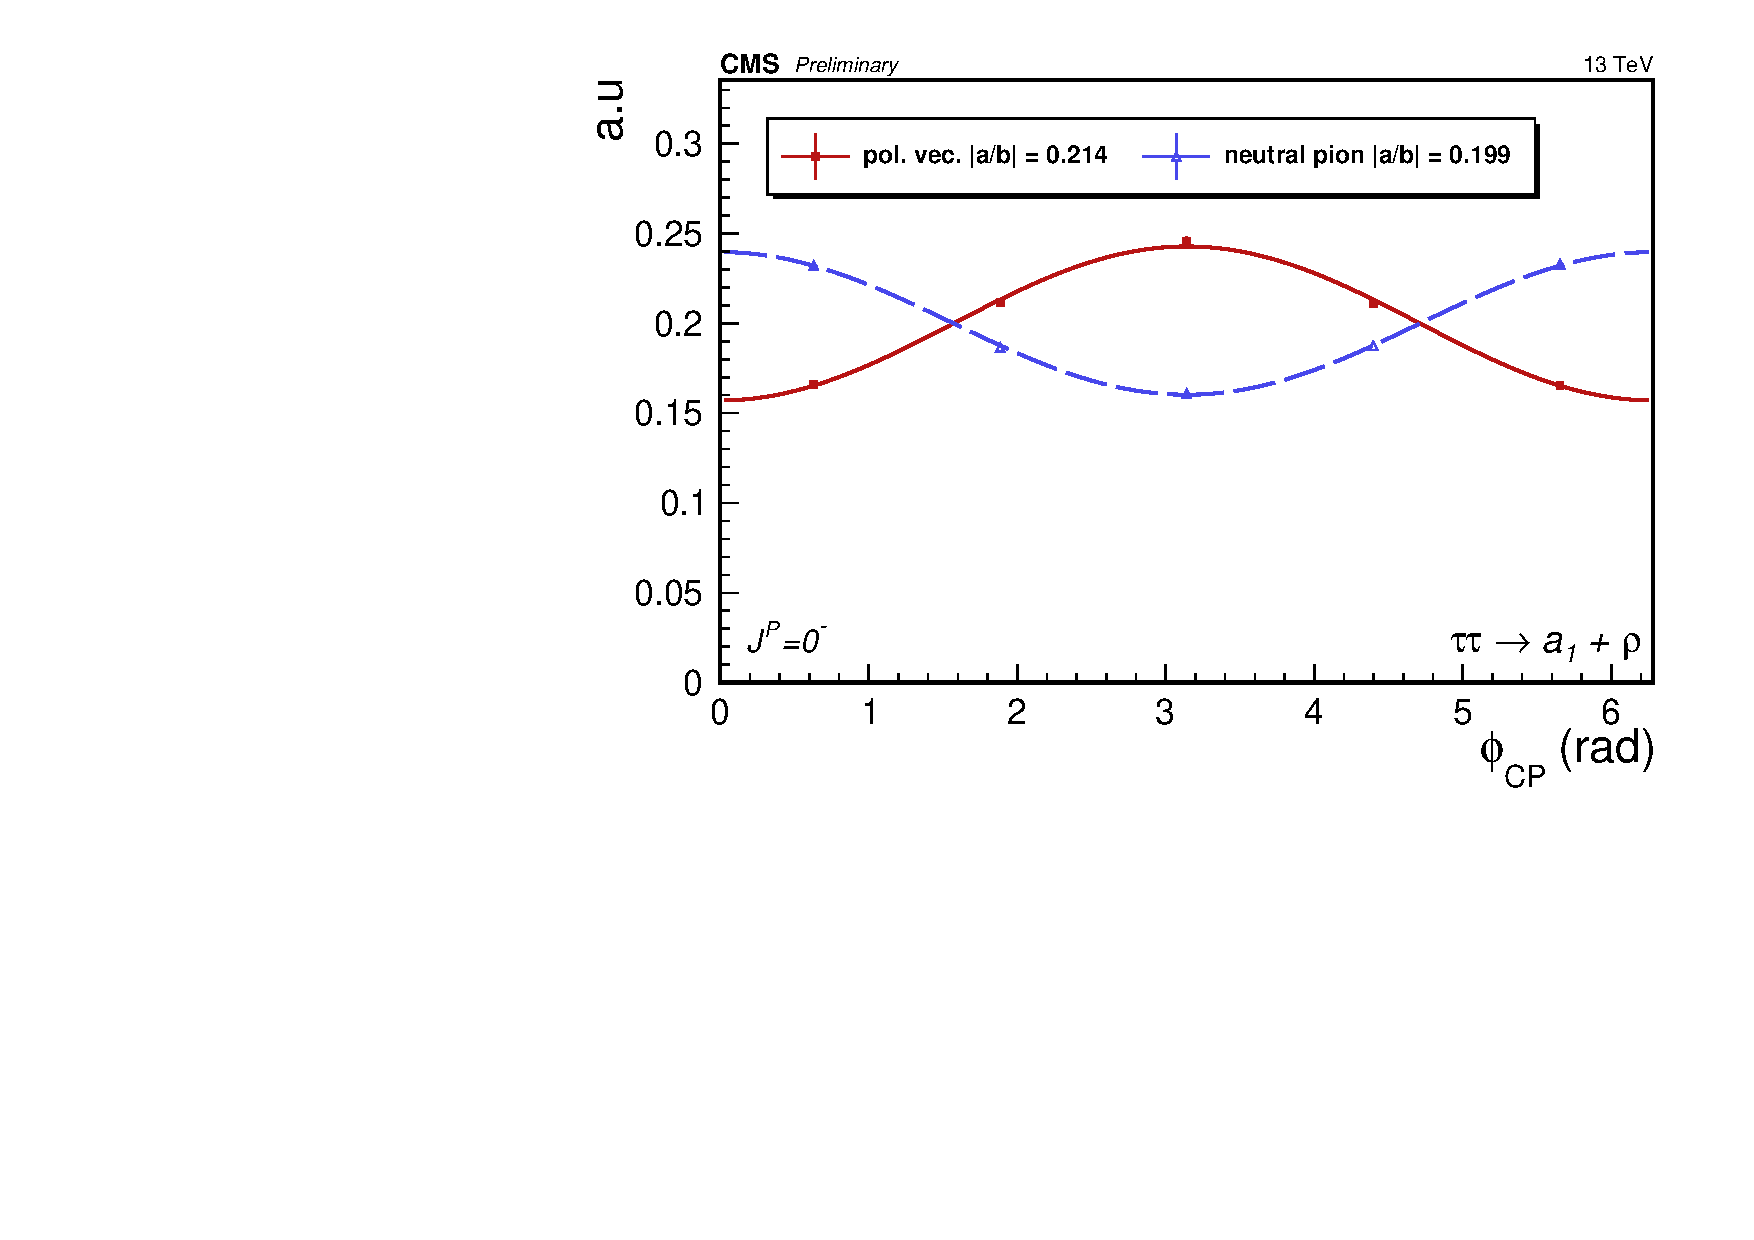
\includegraphics[width=\linewidth]{Chapitre6/Images/A1RHO/A1RHO_odd_reco.pdf} 
    \caption*{} 
    \vspace{10mm}
  \end{subfigure} 

    \begin{subfigure}[b]{0.5\linewidth}
    \centering
    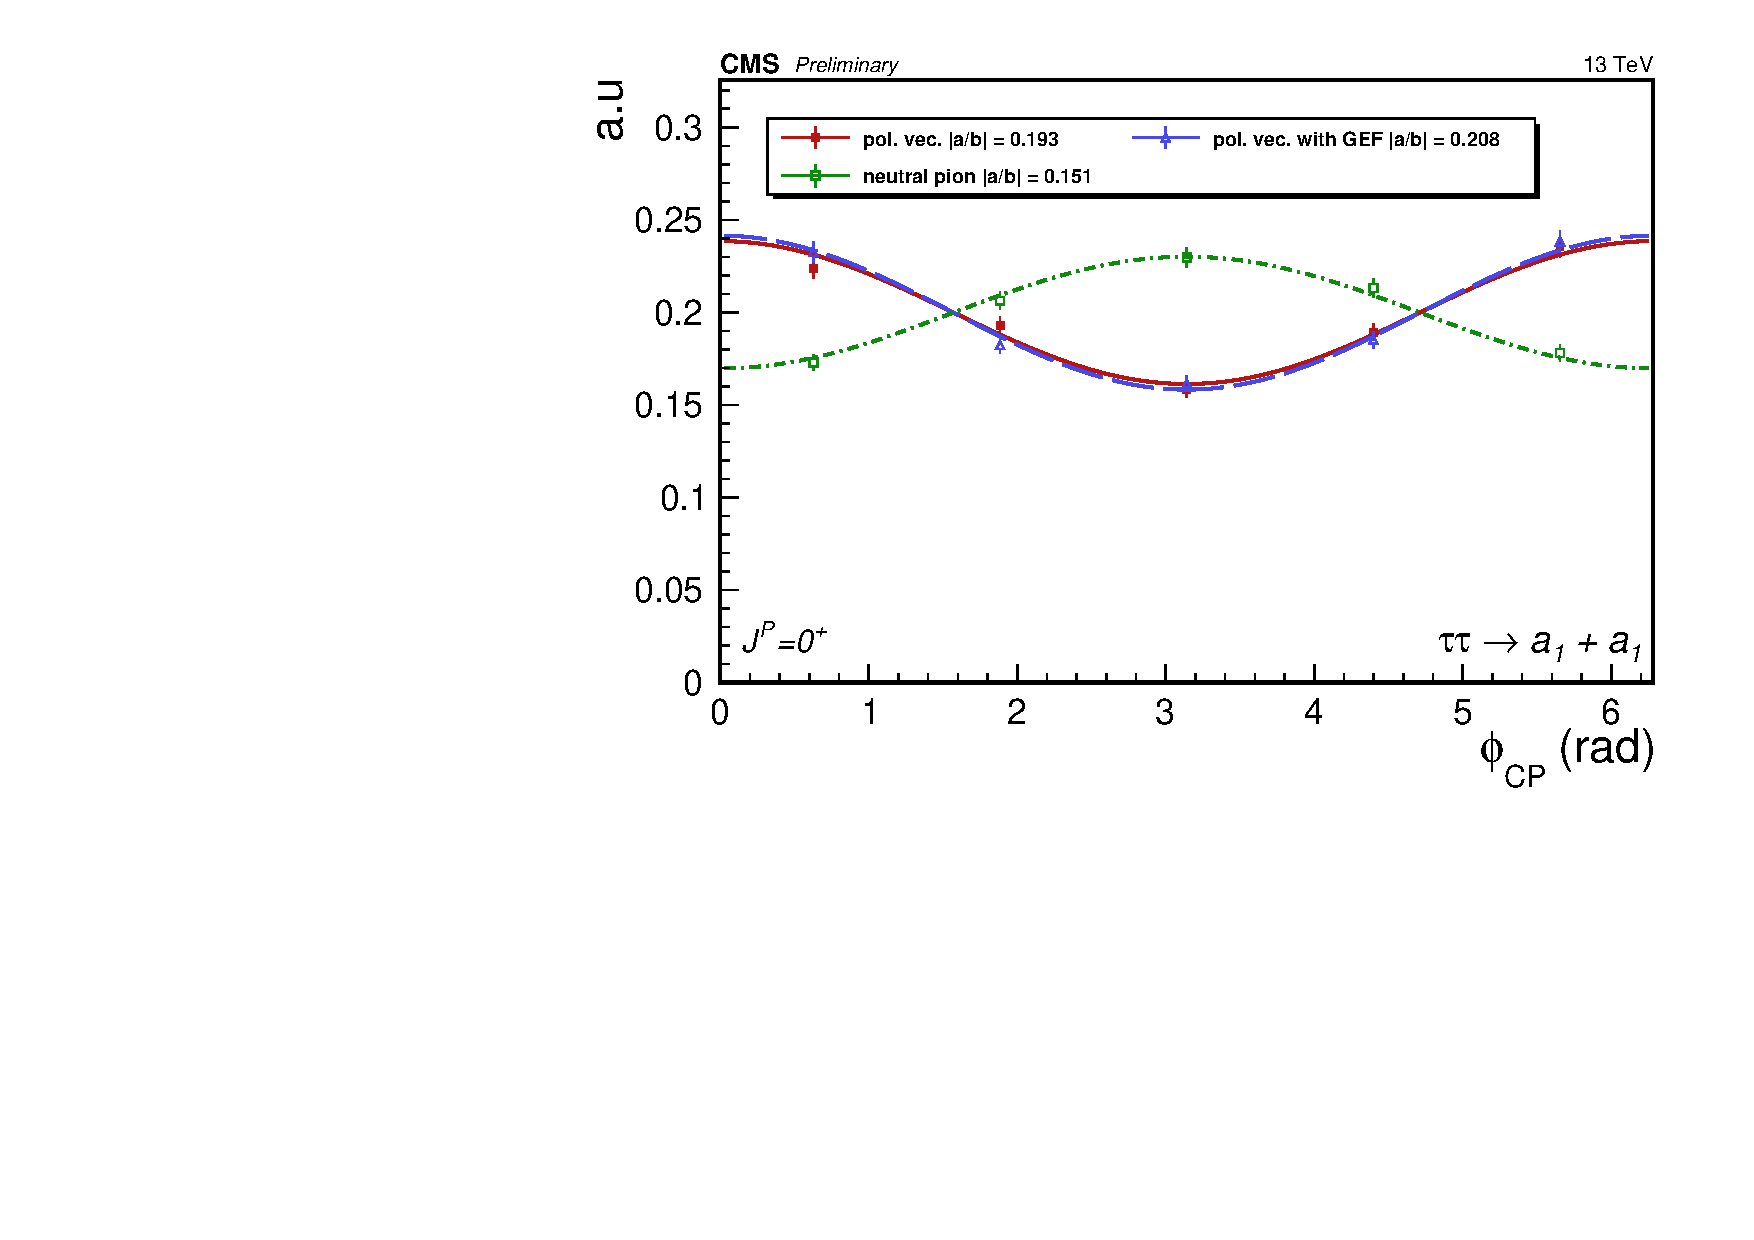
\includegraphics[width=\linewidth]{Chapitre6/Images/A1A1/A1A1_even_reco.pdf} 
    \caption*{} 
    \vspace{0.5ex}
  \end{subfigure}%% 
  \begin{subfigure}[b]{0.5\linewidth}
    \centering
    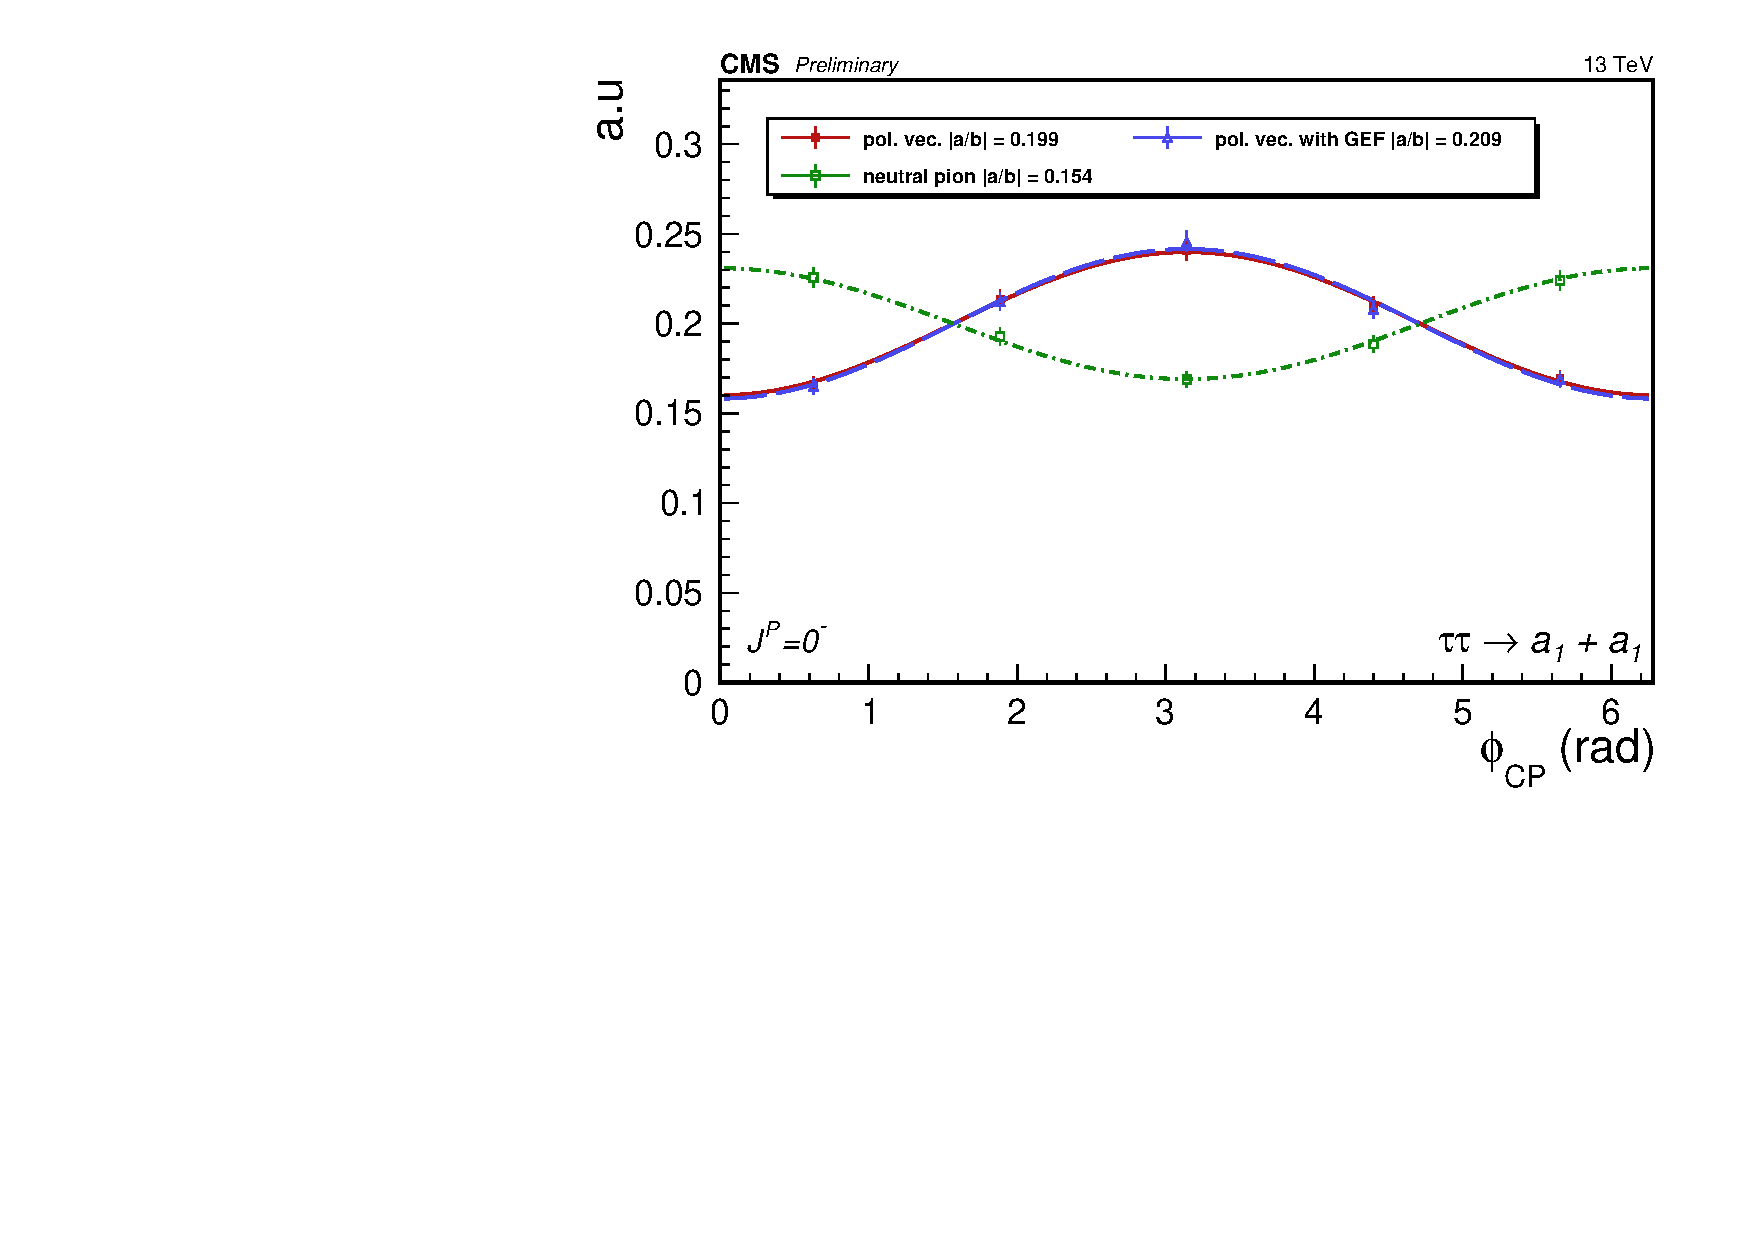
\includegraphics[width=\linewidth]{Chapitre6/Images/A1A1/A1A1_odd_reco.pdf} 
    \caption*{} 
    \vspace{0.5ex}
  \end{subfigure} 
  
  \caption{Distributions de $\phi_{CP}$ dans les canaux $\tau_h\tau_h\rightarrow X+a_1^{3pr}$, avec $X=\pi,\rho,a^{3pr}_1$, au niveau reconstruit pour l'état CP pair (gauche) et CP impair (droite) dans des évènements $ggH\to\tau\tau$.}
  \label{CPreco}
\end{figure}

Cette méthode permet d'obtenir une oscillation dans la distribution de $\phi_{CP}$ avec le vecteur polarimétrique dans tous les canaux hadroniques, à l'exception du canal $\tau_h\tau_h\rightarrow\pi\pi$ dans lequel aucune amélioration n'est de toute façon attendue d'après les résultats précédents. Dans un premier temps, la figure \ref{ZMFreco} montre que l'amplitude d'oscillation au niveau reconstruit avec la méthode du vecteur polarimétrique n'est pas impactée de manière significative par le choix du référentiel au repos dans lequel l'angle $\phi_{CP}$ est calculé. La figure \ref{CPrecoXPI} présente les résultats dans les canaux $\tau_h\tau_h\rightarrow\rho\rho,\pi\rho$, où les performances de la méthode du vecteur polarimétrique restent moindre que celles atteintes avec les méthodes initiales. La figure \ref{CPreco} présente quant à elle les résultats dans les canaux impliquant une résonance $a_1$, où les performances du vecteur polarimétrique sont comparables à celles des autres méthodes. Une amélioration notable est observée dans le canal $a_1a_1$, où les performances sont également comparées à celles de l'algorithme GEF notamment utilisé dans les résultats de thèse de Guillaume Bourgatte \cite{guigui}. \\


\subsection{Limites}


\begin{figure}[!b]
    \centering
    \includegraphics[scale=0.6]{Chapitre6/Images/genprog_evenrhorho.pdf} 
  \caption{Impact progressif de la reconstruction du système di-tau et des produits de désintégration visibles sur l'amplitude d'oscillation dans la distribution de $\phi_{CP}$ dans le canal $\rho\rho$ avec un boson de Higgs produit par fusion de gluons. La distribution pour la méthode du pion neutre au niveau reconstruit est présentée en vert. La distribution pour la méthode du vecteur polarimétrique au niveau généré (reconstruit) est présentée en jaune (rouge) avec le label PV gen. level (PV reco. level).}
  \label{smearingtaus}
\end{figure}

En conclusion, le résultats précédents montrent qu'une amélioration globale de la sensibilité à l'état CP du boson de Higgs est possible dans tous les canaux hadroniques où la méthode du pion neutre peut être remplacée par le vecteur polarimétrique. La limite principale provient de la reconstruction des leptons tau entraînant une forte perte de sensibilité. Toute fois, le facteur dominant dans la dégradation de la sensibilité à l'état CP lors de la reconstruction de l'impulsion du système di-tau reste reste partiellement déterminé à ce stade. La figure \ref{smearingtaus} présente une étude de l'impact de la reconstruction sur l'amplitude de la distribution de $\phi_{CP}$ dans le canal $\rho\rho$. Dans ce canal, les performances du vecteur polarimétrique demeurent moindres que celles de la méthode du pion neutre au niveau reconstruit (Fig. \ref{CPreco}) malgré une amélioration potentielle conséquente observée au niveau généré (Fig. \ref{CPgen)}). À partir du niveau généré, des éléments au niveau reconstruit ont progressivement été remplacés afin de comprendre lesquels jouent un rôle déterminant dans la conservation de la sensibilité. On remarque alors que la conservation des leptons tau au niveau généré et le remplacement des pions de l'état final par ceux au niveau reconstruit (2 generated $\tau$) entraîne la perte de sensibilité minimale avec le niveau généré complet (PV gen. level). A l'inverse, la conservation des pions au niveau généré et le remplacement au niveau reconstruit d'un seul lepton tau (1 generated $\tau$) ou des deux (Generated $\pi$'s) entraîne une perte de sensibilité plus importante que dans le cas précédent mais équivalente pour un seul ou deux leptons tau. Enfin, une dégradation (\textit{smearing}) volontaire de la résolution de chaque composante du quadrivecteur des leptons tau au niveau généré à également été introduite afin de mesurer leur impact individuellement et de manière combinatoire. Ce smearing est introduit en ajoutant une erreur aléatoire à la composante générée de chaque lepton tau selon une distribution gaussienne de largeur semblable à la résolution de reconstruction de l'algorithme SVFit pour les composantes d'énergie et d'impulsion et de FastMTT pour les composantes angulaires (Fig. \ref{TauRes}). On note en particulier que le smearing de la composante $\eta$ (Smeared $\eta$) entraîne la perte de sensibilité la plus significative, suivie du smearing de l'énergie (Smeared $E$) et du smearing de la composante $\phi$ (Smeared $\phi$) avec l'effet le moins important. La perte de sensibilité provoquée par tout autre smearing simultané de plusieurs composantes incluant un smearing de la composante $\eta$ est alors dominée par la perte de résolution sur cette dernière.

\section{Étude du canal $a_1^{3pr}\mu$}

Cette section constitue une introduction au chapitre suivant dans lequel une mesure de l'angle de mélange $\alpha^{H\tau\tau}$ est réalisée dans le canal $a_1^{3pr}\mu$. Une brève étude des autres canaux semi-leptoniques $\pi\mu$ et $\rho\mu$ est également présentée. Dans les canaux $a_1^{3pr}\mu$ et $\rho\mu$, la méthode du paramètre d'impact est employée sur le muon et seulement la méthode du pion neutre employée sur la résonance hadronique est remplacée par la méthode du vecteur polarimétrique. Dans le cas du canal $\pi\mu$, le vecteur polarimétrique remplace la méthode du paramètre d'impact sur le pion. La figure \ref{Xmugen} montre la distribution de $\phi_{CP}$ au niveau générateur pour les canaux $\pi\mu$ et $\rho\mu$. Pour le premier, les résultats montrent qu'aucune amélioration n'est obtenue avec le vecteur polarimétrique, de façon équivalente au canal $\pi\pi$ (Fig. \ref{CPgenPIPI}). Dans le second, une amélioration de l'amplitude de l'ordre de $30\%$ est observée. Cependant, à défaut d'un algorithme de reconstruction de l'impulsion des leptons tau avec de meilleures performances que celles présentées précédemment, cette amélioration est perdue au niveau reconstruit.  \\

\begin{figure}
  \begin{subfigure}[b]{0.5\linewidth}
    \centering
    \includegraphics[width=\linewidth]{Chapitre6/Images/PIMU/pimu_pvdpgen.pdf} 
    \caption*{} 
    \vspace{0.5ex}
  \end{subfigure}%% 
  \begin{subfigure}[b]{0.5\linewidth}
    \centering
    \includegraphics[width=\linewidth]{Chapitre6/Images/RHOMU/rhomu_pvdpgen.pdf} 
    \caption*{} 
    \vspace{0.5ex}
  \end{subfigure} 
\caption{Gauche : distributions de $\phi_{CP}$ au niveau générateur dans le canal $\pi\mu$. Comparaison de l'amplitude d'oscillation pour les états CP pair et impair entre la méthode du paramètre d'impact et le vecteur polarimétrique dans des évènements $ggH\to\tau\tau$. Droite : distributions de $\phi_{CP}$ au niveau générateur dans le canal $\rho\mu$. Comparaison de l'amplitude d'oscillation pour les états CP pair et impair entre la méthode du pion neutre et le vecteur polarimétrique dans des évènements $ggH\to\tau\tau$.}
\label{Xmugen}
\end{figure}


La figure \ref{a1mugen} montre les performances du vecteur polarimétrique au niveau générateur pour le canal $a_1^{3pr}\mu$. L'amplitude moyenne $|a/b|$ de la distribution de $\phi_{CP}$ entre les états CP pair et impair est de $0.058$ pour la méthode du pion neutre combinée à celle du paramètre d'impact, tandis qu'elle est de $0.204$ pour celle du vecteur polarimétrique, représentant une amélioration de l'ordre de $250\%$. La figure présente aussi la distribution de $\phi_{CP}$ pour la désintégration $Z\to\tau\tau$ dans les échantillons \textit{embedded}. La figure \ref{a1mureco} présente les mêmes distributions au niveau reconstruit. L'algorithme utilisé pour la reconstruction de l'impulsion totale des leptons tau et l'application de la méthode du vecteur polarimétrique est l'algorithme GEF introduit dans la section \ref{GEF}. Ces algorithme s'appuie notamment sur l'utilisation du vertex secondaire du lepton tau, dont la position est calculée à partir des traces de pions chargés issus de la désintégration de la résonance, et dont la résolution de reconstruction est présentée dans la figure \ref{SVreso}. L'amélioration moyenne de l'amplitude entre états CP pair et impair apportée par l'utilisation du vecteur polarimétrique est de $63\%$ au niveau reconstruit. \\

\begin{figure}[]
  \begin{subfigure}[b]{0.5\linewidth}
    \centering
    \includegraphics[width=\linewidth]{Chapitre6/Images/A1MU/a1mu_pvdpgen.pdf} 
    \caption*{} 
    \vspace{0.5ex}
  \end{subfigure}%% 
  \begin{subfigure}[b]{0.5\linewidth}
    \centering
    \includegraphics[width=\linewidth]{Chapitre6/Images/A1MU/a1mu_genpv.pdf} 
    \caption*{} 
    \vspace{0.5ex}
  \end{subfigure} 
\caption{Gauche : distributions de $\phi_{CP}$ au niveau générateur dans le canal $a_1^{3pr}\mu$ dans des évènements $ggH\to\tau\tau$. Comparaison de l'amplitude d'oscillation pour les états CP pair et impair entre la méthode du pion neutre et le vecteur polarimétrique. Droite : distribution pour les états CP pair et impair dans des évènements $Z\to\tau\tau$ \textit{embedded} avec le vecteur polarimétrique au niveau généré.}
\label{a1mugen}
\end{figure}

\begin{figure}[]
  \begin{subfigure}[b]{0.5\linewidth}
    \centering
    \includegraphics[width=\linewidth]{Chapitre6/Images/A1MU/a1mu_pvdpreco.pdf} 
    \caption*{} 
    \vspace{0.5ex}
  \end{subfigure}%% 
  \begin{subfigure}[b]{0.5\linewidth}
    \centering
    \includegraphics[width=\linewidth]{Chapitre6/Images/A1MU/a1mu_pv.pdf} 
    \caption*{} 
    \vspace{0.5ex}
  \end{subfigure} 
\caption{Gauche : distributions de $\phi_{CP}$ au niveau reconstruit dans le canal $a_1^{3pr}\mu$. Comparaison de l'amplitude d'oscillation pour les états CP pair et impair entre la méthode du pion neutre et le vecteur polarimétrique. Droite : distribution pour les états CP pair et impair dans des évènements $Z\to\tau\tau$ \textit{embedded} avec le vecteur polarimétrique au niveau reconstruit.}
\label{a1mureco}
\end{figure}

\begin{figure}
    \begin{subfigure}[b]{0.5\linewidth}
    \centering
    \includegraphics[scale=0.19]{Chapitre6/Images/SVx.png} 
    \caption*{} 
    %\vspace{0.5ex}
  \end{subfigure}%% 
  \begin{subfigure}[b]{0.5\linewidth}
    \centering
    \includegraphics[scale=0.19]{Chapitre6/Images/SVy.png} 
    \caption*{} 
    %\vspace{0.5ex}
  \end{subfigure}
  
  \begin{subfigure}[b]{\linewidth}
    \centering
    \includegraphics[scale=0.19]{Chapitre6/Images/SVz.png} 
    \caption*{} 
    %\vspace{0.5ex}
  \end{subfigure}

\caption{Résolution de la reconstruction du vertex secondaire du lepton tau $\tau_h\to a_1^{3pr}$ dans des événements $ggH\to\tau\tau$.}
\label{SVreso}
\end{figure}

La distribution de $\phi_{CP}$ dans les évènements $Z\to\tau\tau$ \textit{embedded} semble présenter une légère oscillation autour de la valeur moyenne au niveau reconstruit avec deux minima en $\pi/2$ et $3\pi/2$. Cette oscillation n'étant pas d'origine physique, elle peut toutefois être induite par un alignement imparfait du détecteur réel et du détecteur simulé lors de la phase de regroupement de la procédure d'\textit{embedding} auquel le vecteur polarimétrique serait d'avantage sensible. Afin de s'assurer que l'utilisation des échantillons \textit{embedded} n'entraîne pas de biais, les distributions de $\phi_{CP}$ dans le canal $a_1^{3pr}\mu$ au niveau généré et reconstruit sont comparées dans la figure \ref{embflatness}. Ces résultats montrent notamment que la distribution de $\phi_{CP}$ est plate au niveau généré pour chaque méthode, bien qu'un biais induit par une erreur d'alignement des détecteurs devrait en principe être visible si existant. La comparaison de ces distributions au niveau reconstruit montre qu'une légère fluctuation autour de la valeur moyenne existe également pour la méthode du pion neutre (\textit{decay plane}) et ne semble pas indiquer de biais supplémentaire pour le vecteur polarimétrique.

\begin{figure}[!ht]
  \begin{subfigure}[b]{0.5\linewidth}
    \centering
    \includegraphics[width=\linewidth]{Chapitre6/Images/A1MU/gena1muemb.pdf} 
    \caption{} 
    \vspace{0.5ex}
  \end{subfigure}%% 
  \begin{subfigure}[b]{0.5\linewidth}
    \centering
    \includegraphics[width=\linewidth]{Chapitre6/Images/A1MU/recoa1muemb.pdf} 
    \caption{} 
    \vspace{0.5ex}
  \end{subfigure}%% 
  \caption{Distributions de $\phi_{CP}$ dans le canal $a_1^{3pr}\mu$ dans un échantillon \textit{embedded} au niveau généré (a) et au niveau reconstruit (b).}
  \label{embflatness}
\end{figure}